\documentclass{book}
\usepackage[a4paper,top=2.5cm,bottom=2.5cm,left=2.5cm,right=2.5cm]{geometry}
\usepackage{makeidx}
\usepackage{natbib}
\usepackage{graphicx}
\usepackage{multicol}
\usepackage{float}
\usepackage{listings}
\usepackage{color}
\usepackage{ifthen}
\usepackage[table]{xcolor}
\usepackage{textcomp}
\usepackage{alltt}
\usepackage{ifpdf}
\ifpdf
\usepackage[pdftex,
            pagebackref=true,
            colorlinks=true,
            linkcolor=blue,
            unicode
           ]{hyperref}
\else
\usepackage[ps2pdf,
            pagebackref=true,
            colorlinks=true,
            linkcolor=blue,
            unicode
           ]{hyperref}
\usepackage{pspicture}
\fi
\usepackage[utf8]{inputenc}
\usepackage{mathptmx}
\usepackage[scaled=.90]{helvet}
\usepackage{courier}
\usepackage{sectsty}
\usepackage{amssymb}
\usepackage[titles]{tocloft}
\usepackage{doxygen}
\lstset{language=C++,inputencoding=utf8,basicstyle=\footnotesize,breaklines=true,breakatwhitespace=true,tabsize=4,numbers=left }
\makeindex
\setcounter{tocdepth}{3}
\renewcommand{\footrulewidth}{0.4pt}
\renewcommand{\familydefault}{\sfdefault}
\hfuzz=15pt
\setlength{\emergencystretch}{15pt}
\hbadness=750
\tolerance=750
\begin{document}
\hypersetup{pageanchor=false,citecolor=blue}
\begin{titlepage}
\vspace*{7cm}
\begin{center}
{\Large Ba\-Ka\-Plan \\[1ex]\large Version 0.\-6 }\\
\vspace*{1cm}
{\large Generated by Doxygen 1.8.1.2}\\
\vspace*{0.5cm}
{\small Thu Mar 14 2013 23:57:19}\\
\end{center}
\end{titlepage}
\clearemptydoublepage
\pagenumbering{roman}
\tableofcontents
\clearemptydoublepage
\pagenumbering{arabic}
\hypersetup{pageanchor=true,citecolor=blue}
\chapter{Class Index}
\section{\-Class \-Hierarchy}
\-This inheritance list is sorted roughly, but not completely, alphabetically\-:\begin{DoxyCompactList}
\item \contentsline{section}{\-Database}{\pageref{de/d03/classDatabase}}{}
\item \contentsline{section}{\-Data\-Sheet}{\pageref{dd/dcc/classDataSheet}}{}
\item \contentsline{section}{\-Exapand\-Roll\-No}{\pageref{d2/d9b/classExapandRollNo}}{}
\item \contentsline{section}{\-Input\-Detail}{\pageref{db/d6e/classInputDetail}}{}
\begin{DoxyCompactList}
\item \contentsline{section}{\-Class\-Detail}{\pageref{d9/ddf/classClassDetail}}{}
\item \contentsline{section}{\-Date\-Sheet}{\pageref{de/d0e/classDateSheet}}{}
\item \contentsline{section}{\-Exam\-Detail}{\pageref{df/d4d/classExamDetail}}{}
\begin{DoxyCompactList}
\item \contentsline{section}{\-Valid\-Strategy}{\pageref{d9/d15/classValidStrategy}}{}
\end{DoxyCompactList}
\item \contentsline{section}{\-Login}{\pageref{dd/dfd/classLogin}}{}
\begin{DoxyCompactList}
\item \contentsline{section}{\-Project\-Detail}{\pageref{d3/dd8/classProjectDetail}}{}
\end{DoxyCompactList}
\item \contentsline{section}{\-Report}{\pageref{da/da8/classReport}}{}
\item \contentsline{section}{\-Roll\-No\-Detail}{\pageref{d6/db0/classRollNoDetail}}{}
\item \contentsline{section}{\-Room\-Detail}{\pageref{d4/de5/classRoomDetail}}{}
\item \contentsline{section}{\-Strategy}{\pageref{d2/df2/classStrategy}}{}
\end{DoxyCompactList}
\item \contentsline{section}{\-Input\-Field\-Name}{\pageref{dd/db2/classInputFieldName}}{}
\item \contentsline{section}{\-Java\-Script}{\pageref{da/dac/classJavaScript}}{}
\item \contentsline{section}{\-Page\-Structure\-Maker}{\pageref{de/d88/classPageStructureMaker}}{}
\begin{DoxyCompactList}
\item \contentsline{section}{\-Page\-Layout}{\pageref{d7/d9e/classPageLayout}}{}
\end{DoxyCompactList}
\item \contentsline{section}{\-Read\-Input}{\pageref{de/d50/classReadInput}}{}
\begin{DoxyCompactList}
\item \contentsline{section}{\-Arrange\-Roll\-No}{\pageref{da/de9/classArrangeRollNo}}{}
\begin{DoxyCompactList}
\item \contentsline{section}{\-Date\-Sheet}{\pageref{de/d0e/classDateSheet}}{}
\end{DoxyCompactList}
\item \contentsline{section}{\-Expand\-Roll\-No}{\pageref{d0/d6e/classExpandRollNo}}{}
\item \contentsline{section}{\-Seat\-Plan}{\pageref{d2/d41/classSeatPlan}}{}
\begin{DoxyCompactList}
\item \contentsline{section}{\-Strategy}{\pageref{d2/df2/classStrategy}}{}
\end{DoxyCompactList}
\end{DoxyCompactList}
\item \contentsline{section}{\-Read\-Input\-Field}{\pageref{d8/d37/classReadInputField}}{}
\item \contentsline{section}{\-Send\-Mail}{\pageref{d6/d66/classSendMail}}{}
\end{DoxyCompactList}

\chapter{Class Index}
\section{Class List}
Here are the classes, structs, unions and interfaces with brief descriptions\-:\begin{DoxyCompactList}
\item\contentsline{section}{\hyperlink{classArrangeRollNo}{Arrange\-Roll\-No} }{\pageref{classArrangeRollNo}}{}
\item\contentsline{section}{\hyperlink{classBranchDetails}{Branch\-Details} }{\pageref{classBranchDetails}}{}
\item\contentsline{section}{\hyperlink{classBranchReport}{Branch\-Report} }{\pageref{classBranchReport}}{}
\item\contentsline{section}{\hyperlink{classExamDetails}{Exam\-Details} }{\pageref{classExamDetails}}{}
\item\contentsline{section}{\hyperlink{classExapandRollNo}{Exapand\-Roll\-No} }{\pageref{classExapandRollNo}}{}
\item\contentsline{section}{\hyperlink{classHome}{Home} }{\pageref{classHome}}{}
\item\contentsline{section}{\hyperlink{classHomeCSS}{Home\-C\-S\-S} }{\pageref{classHomeCSS}}{}
\item\contentsline{section}{\hyperlink{classHTMLTags}{H\-T\-M\-L\-Tags} \\*Base class containong Basic Html Tags and methods }{\pageref{classHTMLTags}}{}
\item\contentsline{section}{\hyperlink{classReadBranchDetails}{Read\-Branch\-Details} }{\pageref{classReadBranchDetails}}{}
\item\contentsline{section}{\hyperlink{classReadExamDetails}{Read\-Exam\-Details} }{\pageref{classReadExamDetails}}{}
\item\contentsline{section}{\hyperlink{classReadInput}{Read\-Input} }{\pageref{classReadInput}}{}
\item\contentsline{section}{\hyperlink{classReadRollNoDetails}{Read\-Roll\-No\-Details} }{\pageref{classReadRollNoDetails}}{}
\item\contentsline{section}{\hyperlink{classReadRoomDetails}{Read\-Room\-Details} }{\pageref{classReadRoomDetails}}{}
\item\contentsline{section}{\hyperlink{classReport}{Report} }{\pageref{classReport}}{}
\item\contentsline{section}{\hyperlink{classRollNoDetails}{Roll\-No\-Details} }{\pageref{classRollNoDetails}}{}
\item\contentsline{section}{\hyperlink{classRoomDetails}{Room\-Details} }{\pageref{classRoomDetails}}{}
\item\contentsline{section}{\hyperlink{classRoomReport}{Room\-Report} }{\pageref{classRoomReport}}{}
\item\contentsline{section}{\hyperlink{classSeatPlan}{Seat\-Plan} }{\pageref{classSeatPlan}}{}
\item\contentsline{section}{\hyperlink{classStrategy}{Strategy} }{\pageref{classStrategy}}{}
\item\contentsline{section}{\hyperlink{classSubjectWiseRollNo}{Subject\-Wise\-Roll\-No} }{\pageref{classSubjectWiseRollNo}}{}
\item\contentsline{section}{\hyperlink{classValidation}{Validation} }{\pageref{classValidation}}{}
\end{DoxyCompactList}

\chapter{Class Documentation}
\hypertarget{classClassDetail}{\section{Class\-Detail Class Reference}
\label{classClassDetail}\index{Class\-Detail@{Class\-Detail}}
}


For getting class details nd reading projectdetail.  




{\ttfamily \#include $<$class.\-h$>$}

Inheritance diagram for Class\-Detail\-:\begin{figure}[H]
\begin{center}
\leavevmode
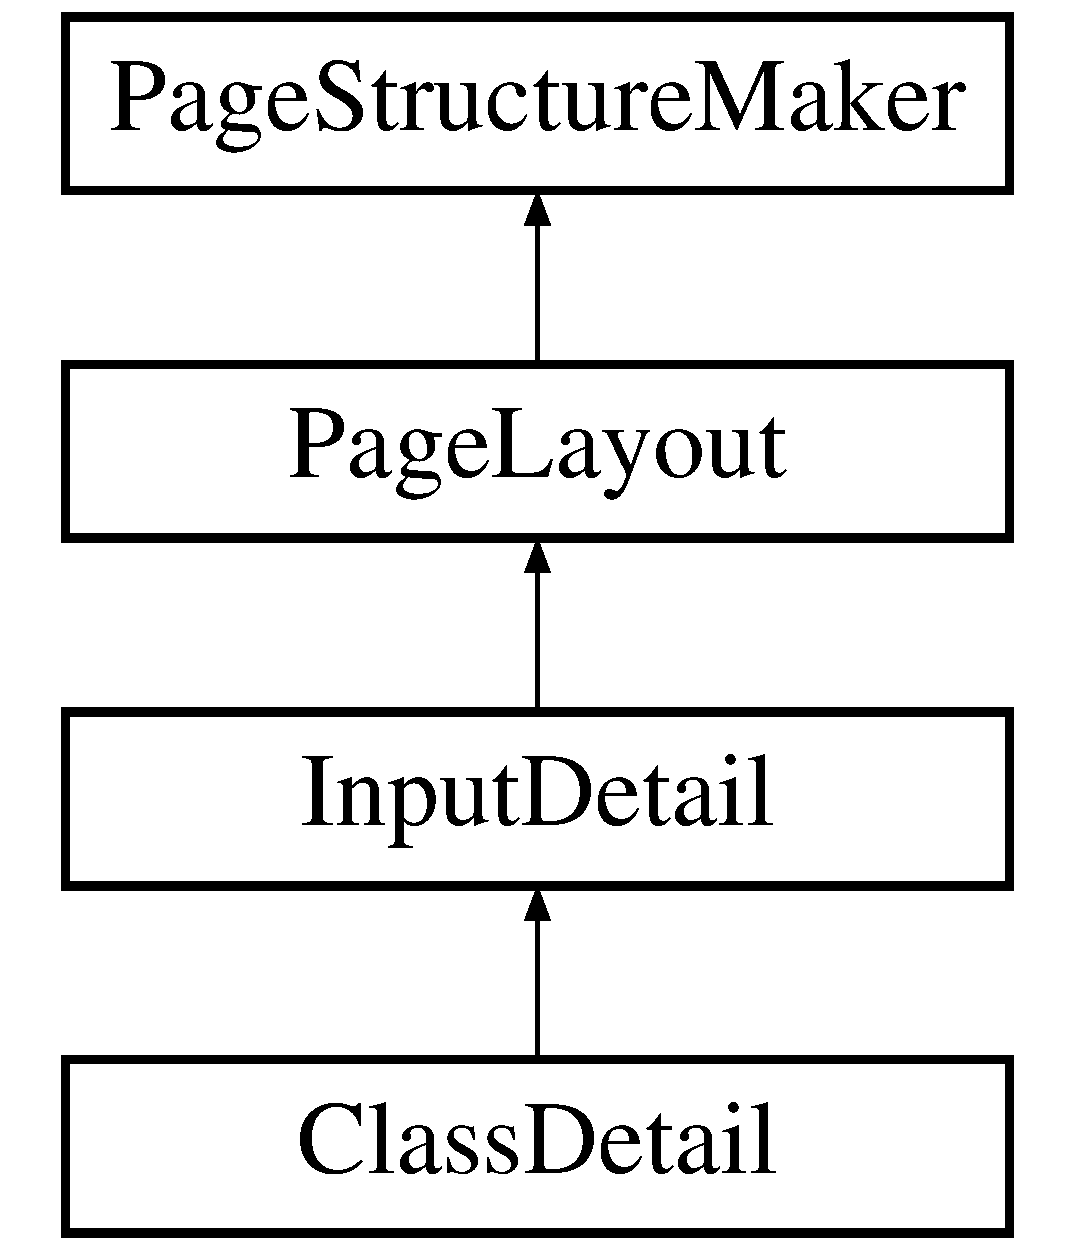
\includegraphics[height=2.000000cm]{classClassDetail}
\end{center}
\end{figure}
\subsection*{Public Member Functions}
\begin{DoxyCompactItemize}
\item 
\hyperlink{classClassDetail_a70975c4ff964e21958e31f2020cdc643}{Class\-Detail} ()
\begin{DoxyCompactList}\small\item\em Constructor. \end{DoxyCompactList}\item 
void \hyperlink{classClassDetail_a2e2384f482bb2dca5f2d8a1c27491ae9}{Set\-Default\-Value} ()
\begin{DoxyCompactList}\small\item\em Setting default values of text fields (classname, subject name, subject code) \end{DoxyCompactList}\item 
void \hyperlink{classClassDetail_a360bb591c7b1559d1b6bac0609dbad1e}{Project\-Type} ()
\begin{DoxyCompactList}\small\item\em For reading project type ie old or new then calling Old\-Project and New\-Project func. accord to that. \end{DoxyCompactList}\item 
void \hyperlink{classClassDetail_af8cb05bf1c3d5581edddcdab96def081}{Old\-Project} ()
\begin{DoxyCompactList}\small\item\em This func. is called is project type = Old. \end{DoxyCompactList}\item 
void \hyperlink{classClassDetail_a521c8e315fa844a04932382ae85335bf}{New\-Project} ()
\begin{DoxyCompactList}\small\item\em This func tis called if Project\-Type = New. \end{DoxyCompactList}\item 
void \hyperlink{classClassDetail_a645fe4306391def818cdadbdc3febbf7}{Class\-Detail\-Page} (string \hyperlink{classInputDetail_a1abb16cd695678c3fa05e3c812823fee}{msg}=\char`\"{}\char`\"{})
\begin{DoxyCompactList}\small\item\em function for displaying html page for class details \end{DoxyCompactList}\item 
\hyperlink{classClassDetail_a2aeaf33b0a277a897aad308cffde211a}{$\sim$\-Class\-Detail} ()
\begin{DoxyCompactList}\small\item\em Destructor. \end{DoxyCompactList}\end{DoxyCompactItemize}
\subsection*{Protected Attributes}
\begin{DoxyCompactItemize}
\item 
\hypertarget{classClassDetail_af920fe4a369c37b9b48b1c4a5451b99c}{\hyperlink{classProjectDetail}{Project\-Detail} {\bfseries project}}\label{classClassDetail_af920fe4a369c37b9b48b1c4a5451b99c}

\item 
\hypertarget{classClassDetail_ae990299c6643a8d4f958585e790d0dc8}{S\-T\-R\-I\-N\-G\-\_\-\-V\-E\-C {\bfseries value}}\label{classClassDetail_ae990299c6643a8d4f958585e790d0dc8}

\end{DoxyCompactItemize}


\subsection{Detailed Description}
For getting class details nd reading projectdetail. 

Include \hyperlink{class_8h}{class.\-h}

Include \hyperlink{project_8h_source}{project.\-h} 

Definition at line 30 of file class.\-h.



\subsection{Constructor \& Destructor Documentation}
\hypertarget{classClassDetail_a70975c4ff964e21958e31f2020cdc643}{\index{Class\-Detail@{Class\-Detail}!Class\-Detail@{Class\-Detail}}
\index{Class\-Detail@{Class\-Detail}!ClassDetail@{Class\-Detail}}
\subsubsection[{Class\-Detail}]{\setlength{\rightskip}{0pt plus 5cm}Class\-Detail\-::\-Class\-Detail (
\begin{DoxyParamCaption}
{}
\end{DoxyParamCaption}
)}}\label{classClassDetail_a70975c4ff964e21958e31f2020cdc643}


Constructor. 

Constructor 

Definition at line 27 of file class.\-cc.

\hypertarget{classClassDetail_a2aeaf33b0a277a897aad308cffde211a}{\index{Class\-Detail@{Class\-Detail}!$\sim$\-Class\-Detail@{$\sim$\-Class\-Detail}}
\index{$\sim$\-Class\-Detail@{$\sim$\-Class\-Detail}!ClassDetail@{Class\-Detail}}
\subsubsection[{$\sim$\-Class\-Detail}]{\setlength{\rightskip}{0pt plus 5cm}Class\-Detail\-::$\sim$\-Class\-Detail (
\begin{DoxyParamCaption}
{}
\end{DoxyParamCaption}
)}}\label{classClassDetail_a2aeaf33b0a277a897aad308cffde211a}


Destructor. 

D\-Estructor 

Definition at line 319 of file class.\-cc.



\subsection{Member Function Documentation}
\hypertarget{classClassDetail_a645fe4306391def818cdadbdc3febbf7}{\index{Class\-Detail@{Class\-Detail}!Class\-Detail\-Page@{Class\-Detail\-Page}}
\index{Class\-Detail\-Page@{Class\-Detail\-Page}!ClassDetail@{Class\-Detail}}
\subsubsection[{Class\-Detail\-Page}]{\setlength{\rightskip}{0pt plus 5cm}void Class\-Detail\-::\-Class\-Detail\-Page (
\begin{DoxyParamCaption}
\item[{string}]{msg = {\ttfamily \char`\"{}\char`\"{}}}
\end{DoxyParamCaption}
)}}\label{classClassDetail_a645fe4306391def818cdadbdc3febbf7}


function for displaying html page for class details 

Class detail page


\begin{DoxyParams}{Parameters}
{\em msg} & For displaying error message if any \\
\hline
\end{DoxyParams}


Definition at line 181 of file class.\-cc.

\hypertarget{classClassDetail_a521c8e315fa844a04932382ae85335bf}{\index{Class\-Detail@{Class\-Detail}!New\-Project@{New\-Project}}
\index{New\-Project@{New\-Project}!ClassDetail@{Class\-Detail}}
\subsubsection[{New\-Project}]{\setlength{\rightskip}{0pt plus 5cm}void Class\-Detail\-::\-New\-Project (
\begin{DoxyParamCaption}
{}
\end{DoxyParamCaption}
)}}\label{classClassDetail_a521c8e315fa844a04932382ae85335bf}


This func tis called if Project\-Type = New. 

New project $<$ If project\-Name already exists 

Definition at line 96 of file class.\-cc.

\hypertarget{classClassDetail_af8cb05bf1c3d5581edddcdab96def081}{\index{Class\-Detail@{Class\-Detail}!Old\-Project@{Old\-Project}}
\index{Old\-Project@{Old\-Project}!ClassDetail@{Class\-Detail}}
\subsubsection[{Old\-Project}]{\setlength{\rightskip}{0pt plus 5cm}void Class\-Detail\-::\-Old\-Project (
\begin{DoxyParamCaption}
{}
\end{DoxyParamCaption}
)}}\label{classClassDetail_af8cb05bf1c3d5581edddcdab96def081}


This func. is called is project type = Old. 

Existing project $<$ If project\-Name already exists 

Definition at line 132 of file class.\-cc.

\hypertarget{classClassDetail_a360bb591c7b1559d1b6bac0609dbad1e}{\index{Class\-Detail@{Class\-Detail}!Project\-Type@{Project\-Type}}
\index{Project\-Type@{Project\-Type}!ClassDetail@{Class\-Detail}}
\subsubsection[{Project\-Type}]{\setlength{\rightskip}{0pt plus 5cm}void Class\-Detail\-::\-Project\-Type (
\begin{DoxyParamCaption}
{}
\end{DoxyParamCaption}
)}}\label{classClassDetail_a360bb591c7b1559d1b6bac0609dbad1e}


For reading project type ie old or new then calling Old\-Project and New\-Project func. accord to that. 

Type of project 

Definition at line 49 of file class.\-cc.

\hypertarget{classClassDetail_a2e2384f482bb2dca5f2d8a1c27491ae9}{\index{Class\-Detail@{Class\-Detail}!Set\-Default\-Value@{Set\-Default\-Value}}
\index{Set\-Default\-Value@{Set\-Default\-Value}!ClassDetail@{Class\-Detail}}
\subsubsection[{Set\-Default\-Value}]{\setlength{\rightskip}{0pt plus 5cm}void Class\-Detail\-::\-Set\-Default\-Value (
\begin{DoxyParamCaption}
{}
\end{DoxyParamCaption}
)}}\label{classClassDetail_a2e2384f482bb2dca5f2d8a1c27491ae9}


Setting default values of text fields (classname, subject name, subject code) 

Set default values 

Definition at line 77 of file class.\-cc.



The documentation for this class was generated from the following files\-:\begin{DoxyCompactItemize}
\item 
frontend/src/header/\hyperlink{class_8h}{class.\-h}\item 
frontend/src/\hyperlink{class_8cc}{class.\-cc}\end{DoxyCompactItemize}

\hypertarget{classDatabase}{\section{Database Class Reference}
\label{classDatabase}\index{Database@{Database}}
}


{\ttfamily \#include $<$database.\-h$>$}

\subsection*{Public Member Functions}
\begin{DoxyCompactItemize}
\item 
\hyperlink{classDatabase_a4703c80e6969d33565ea340f768fdadf}{Database} ()
\item 
void \hyperlink{classDatabase_aec3d0f84e49a58a59f254c90193c1303}{Select\-Query} (string column, string table, vector$<$ string $>$ \&result)
\item 
void \hyperlink{classDatabase_a958467134aa40db133cdf6d46ab52c86}{Select\-Query} (string column, string table, string \&result, string where)
\item 
void \hyperlink{classDatabase_a6fb9e249cb97830af86c00804bb209a2}{Select\-Column} (string query, vector$<$ string $>$ \&result)
\item 
void \hyperlink{classDatabase_a20f7ccadac8f3b67d4344f7da4594eda}{Select\-Project\-I\-D} (string \&project\-I\-D)
\item 
void \hyperlink{classDatabase_a7070d93bf44c5f90504944f54607b9b0}{Insert\-User} (string user\-Email\-I\-D, string user\-Password)
\item 
void \hyperlink{classDatabase_a63d8c1af7507b1dcdc81a411f9a0b4b4}{Insert\-Query} (string query)
\item 
void \hyperlink{classDatabase_a513326ea43b2455177731fbc92c4bf4f}{Insert\-Query} (string column, string value, string table)
\item 
void \hyperlink{classDatabase_a478f862bd338a92b13c2899bb4e28843}{Insert\-Session} (string email\-I\-D, string session\-I\-D)
\item 
void \hyperlink{classDatabase_aae19d9dac16779519f94cc68e29cb57d}{Insert\-Project\-Name} (string email\-I\-D, string project\-Name)
\item 
void \hyperlink{classDatabase_ad6af2dc859cda41dcbdad9cd51f5c38b}{Insert\-Total\-Classes} (string project\-I\-D, string total\-Classes)
\item 
void \hyperlink{classDatabase_a45deae7ea496fccefb9bccd75ea5578a}{Insert\-Class\-Detail} (string project\-I\-D, string class\-Name, string total\-Subjects, string subject\-Name, string subject\-Code)
\item 
void \hyperlink{classDatabase_a8e52c1b853b6f1d96cf7053f0268838d}{Insert\-Total\-Centres} (string project\-I\-D, string total\-Centre)
\item 
void \hyperlink{classDatabase_a8b248d14e1cb2fc4ba2c9da313f385cb}{Insert\-Room\-Detail} (string project\-I\-D, string centre\-Name, string room\-No, string rows, string columns)
\item 
void \hyperlink{classDatabase_a6cd1b1181fb636aff93ba43f0fcd2764}{Insert\-Total\-Rooms} (string project\-I\-D, string centre\-Name, string totalrooms)
\item 
void \hyperlink{classDatabase_a0a1ec932aafeef96637d5ee68ac7898b}{Insert\-Exam\-Detail} (string project\-I\-D, string exam\-Name, string exam\-Date, string exam\-Time, string exam\-Venue)
\item 
void \hyperlink{classDatabase_a6015ae56eb561f579e573be709ef434c}{Insert\-Strategy} (string project\-I\-D, string strategy)
\item 
\hyperlink{classDatabase_a84d399a2ad58d69daab9b05330e1316d}{$\sim$\-Database} ()
\end{DoxyCompactItemize}
\subsection*{Protected Attributes}
\begin{DoxyCompactItemize}
\item 
M\-Y\-S\-Q\-L $\ast$ \hyperlink{classDatabase_aa232b806b05ef654cd5579bca5f1dbad}{connect}
\item 
\hypertarget{classDatabase_ad5921cd2f70d0c22895f2cc5542ab4d7}{M\-Y\-S\-Q\-L\-\_\-\-R\-E\-S $\ast$ {\bfseries res\-\_\-set}}\label{classDatabase_ad5921cd2f70d0c22895f2cc5542ab4d7}

\item 
\hypertarget{classDatabase_a71ad7ae59677936d2ca6666f9de9df40}{M\-Y\-S\-Q\-L\-\_\-\-R\-O\-W {\bfseries row}}\label{classDatabase_a71ad7ae59677936d2ca6666f9de9df40}

\item 
unsigned int \hyperlink{classDatabase_a02965883689dd1d8007c86cebf6df89e}{numrows}
\item 
string \hyperlink{classDatabase_acd64ff0e98b28cd1c6928a1236634521}{t\-Login}
\item 
\hypertarget{classDatabase_aa8ec817b6216079c8e541ec80c8bd4fa}{string {\bfseries t\-Register}}\label{classDatabase_aa8ec817b6216079c8e541ec80c8bd4fa}

\item 
\hypertarget{classDatabase_a62dd3ad69a4a07e66b412e276049ea48}{string {\bfseries t\-Project\-Detail}}\label{classDatabase_a62dd3ad69a4a07e66b412e276049ea48}

\item 
\hypertarget{classDatabase_a1b3174ab4ae9b3cb80448d48817375be}{int {\bfseries i}}\label{classDatabase_a1b3174ab4ae9b3cb80448d48817375be}

\item 
\hypertarget{classDatabase_a5b4fd605238ca66878959f5f3ba647f2}{int {\bfseries j}}\label{classDatabase_a5b4fd605238ca66878959f5f3ba647f2}

\item 
\hypertarget{classDatabase_a851daa5b233ce54d75873631b7b2167a}{string {\bfseries query}}\label{classDatabase_a851daa5b233ce54d75873631b7b2167a}

\end{DoxyCompactItemize}


\subsection{Detailed Description}
-\/-\/-\/-\/-\/-\/-\/-\/-\/-\/-\/-\/-\/-\/-\/-\/-\/-\/-\/-\/-\/-\/-\/-\/-\/-\/-\/-\/-\/-\/-\/-\/-\/-\/-\/-\/-\/-\/-\/-\/-\/-\/-\/-\/-\/-\/-\/-\/-\/-\/-\/-\/-\/-\/-\/-\/-\/-\/-\/-\/-\/-\/-\/-\/-\/-\/-\/ Include \hyperlink{header_8h_source}{header.\-h} and \hyperlink{database_8h_source}{database.\-h} ------------------------------------------------------------------ =================================================================== Class\-: \hyperlink{classDatabase}{Database} Description\-: \hyperlink{classDatabase}{Database} class for database accessability =================================================================== 

Definition at line 34 of file database.\-h.



\subsection{Constructor \& Destructor Documentation}
\hypertarget{classDatabase_a4703c80e6969d33565ea340f768fdadf}{\index{Database@{Database}!Database@{Database}}
\index{Database@{Database}!Database@{Database}}
\subsubsection[{Database}]{\setlength{\rightskip}{0pt plus 5cm}Database\-::\-Database (
\begin{DoxyParamCaption}
{}
\end{DoxyParamCaption}
)}}\label{classDatabase_a4703c80e6969d33565ea340f768fdadf}
\hyperlink{classDatabase}{Database} Constructor

-\/-\/-\/-\/-\/-\/-\/-\/-\/-\/-\/-\/-\/-\/-\/-\/-\/-\/-\/-\/-\/-\/-\/-\/-\/-\/-\/-\/-\/-\/-\/-\/-\/-\/-\/-\/-\/-\/-\/-\/-\/-\/-\/-\/-\/-\/-\/-\/-\/-\/-\/-\/-\/-\/-\/-\/-\/-\/-\/-\/-\/-\/-\/-\/-\/-\/-\/ Include \hyperlink{database_8h_source}{database.\-h} file local header file(declaration of class) ------------------------------------------------------------------ -\/-\/-\/-\/-\/-\/-\/-\/-\/-\/-\/-\/-\/-\/-\/-\/-\/-\/-\/-\/-\/-\/-\/-\/-\/-\/-\/-\/-\/-\/-\/-\/-\/-\/-\/-\/-\/-\/-\/-\/-\/-\/-\/-\/-\/-\/-\/-\/-\/-\/-\/-\/-\/-\/-\/-\/-\/-\/-\/-\/-\/-\/-\/-\/-\/-\/-\/-\/ Class\-: \hyperlink{classDatabase}{Database} Method\-: \hyperlink{classDatabase}{Database} \-:\-: \hyperlink{classDatabase_a4703c80e6969d33565ea340f768fdadf}{Database()} Description\-: Constructor to initialize database conectivity -\/-\/-\/-\/-\/-\/-\/-\/-\/-\/-\/-\/-\/-\/-\/-\/-\/-\/-\/-\/-\/-\/-\/-\/-\/-\/-\/-\/-\/-\/-\/-\/-\/-\/-\/-\/-\/-\/-\/-\/-\/-\/-\/-\/-\/-\/-\/-\/-\/-\/-\/-\/-\/-\/-\/-\/-\/-\/-\/-\/-\/-\/-\/-\/-\/-\/-\/-\/ 

Definition at line 33 of file database.\-cc.

\hypertarget{classDatabase_a84d399a2ad58d69daab9b05330e1316d}{\index{Database@{Database}!$\sim$\-Database@{$\sim$\-Database}}
\index{$\sim$\-Database@{$\sim$\-Database}!Database@{Database}}
\subsubsection[{$\sim$\-Database}]{\setlength{\rightskip}{0pt plus 5cm}Database\-::$\sim$\-Database (
\begin{DoxyParamCaption}
{}
\end{DoxyParamCaption}
)}}\label{classDatabase_a84d399a2ad58d69daab9b05330e1316d}
Select last project Id of project name \hyperlink{classDatabase}{Database} Destructor

-\/-\/-\/-\/-\/-\/-\/-\/-\/-\/-\/-\/-\/-\/-\/-\/-\/-\/-\/-\/-\/-\/-\/-\/-\/-\/-\/-\/-\/-\/-\/-\/-\/-\/-\/-\/-\/-\/-\/-\/-\/-\/-\/-\/-\/-\/-\/-\/-\/-\/-\/-\/-\/-\/-\/-\/-\/-\/-\/-\/-\/-\/-\/-\/-\/-\/-\/-\/ Class\-: \hyperlink{classDatabase}{Database} Method\-: \hyperlink{classDatabase}{Database} \-:\-: \hyperlink{classDatabase_a84d399a2ad58d69daab9b05330e1316d}{$\sim$\-Database()} Description\-: Destructor for closing database connectivity -\/-\/-\/-\/-\/-\/-\/-\/-\/-\/-\/-\/-\/-\/-\/-\/-\/-\/-\/-\/-\/-\/-\/-\/-\/-\/-\/-\/-\/-\/-\/-\/-\/-\/-\/-\/-\/-\/-\/-\/-\/-\/-\/-\/-\/-\/-\/-\/-\/-\/-\/-\/-\/-\/-\/-\/-\/-\/-\/-\/-\/-\/-\/-\/-\/-\/-\/-\/ 

Definition at line 401 of file database.\-cc.



\subsection{Member Function Documentation}
\hypertarget{classDatabase_a45deae7ea496fccefb9bccd75ea5578a}{\index{Database@{Database}!Insert\-Class\-Detail@{Insert\-Class\-Detail}}
\index{Insert\-Class\-Detail@{Insert\-Class\-Detail}!Database@{Database}}
\subsubsection[{Insert\-Class\-Detail}]{\setlength{\rightskip}{0pt plus 5cm}void Database\-::\-Insert\-Class\-Detail (
\begin{DoxyParamCaption}
\item[{string}]{project\-I\-D, }
\item[{string}]{class\-Name, }
\item[{string}]{total\-Subjects, }
\item[{string}]{subject\-Name, }
\item[{string}]{subject\-Code}
\end{DoxyParamCaption}
)}}\label{classDatabase_a45deae7ea496fccefb9bccd75ea5578a}
Insert into \hyperlink{classClassDetail}{Class\-Detail}

--------------------------------------------------------------------\par
 Class\-: \hyperlink{classDatabase}{Database} \par
 Method\-: \hyperlink{classDatabase}{Database} \-:\-: Insert\-Class\-Detail(project\-I\-D, class\-Name, subject\-Name, subject\-Code) \par
 Description\-: Inserting class detail into table \par
 -\/-\/-\/-\/-\/-\/-\/-\/-\/-\/-\/-\/-\/-\/-\/-\/-\/-\/-\/-\/-\/-\/-\/-\/-\/-\/-\/-\/-\/-\/-\/-\/-\/-\/-\/-\/-\/-\/-\/-\/-\/-\/-\/-\/-\/-\/-\/-\/-\/-\/-\/-\/-\/-\/-\/-\/-\/-\/-\/-\/-\/-\/-\/-\/-\/-\/-\/-\/ 

Definition at line 258 of file database.\-cc.

\hypertarget{classDatabase_a0a1ec932aafeef96637d5ee68ac7898b}{\index{Database@{Database}!Insert\-Exam\-Detail@{Insert\-Exam\-Detail}}
\index{Insert\-Exam\-Detail@{Insert\-Exam\-Detail}!Database@{Database}}
\subsubsection[{Insert\-Exam\-Detail}]{\setlength{\rightskip}{0pt plus 5cm}void Database\-::\-Insert\-Exam\-Detail (
\begin{DoxyParamCaption}
\item[{string}]{project\-I\-D, }
\item[{string}]{exam\-Name, }
\item[{string}]{exam\-Date, }
\item[{string}]{exam\-Time, }
\item[{string}]{exam\-Venue}
\end{DoxyParamCaption}
)}}\label{classDatabase_a0a1ec932aafeef96637d5ee68ac7898b}
Insert into exam detail

--------------------------------------------------------------------\par
 Class\-: \hyperlink{classDatabase}{Database} \par
 Method\-: \hyperlink{classDatabase}{Database} \-:\-: Insert\-Total\-Rooms(project\-I\-D, exam\-Name, exam\-Date, exam\-Time, exam\-Venue) \par
 Description\-: store data into exam detail \par
 -\/-\/-\/-\/-\/-\/-\/-\/-\/-\/-\/-\/-\/-\/-\/-\/-\/-\/-\/-\/-\/-\/-\/-\/-\/-\/-\/-\/-\/-\/-\/-\/-\/-\/-\/-\/-\/-\/-\/-\/-\/-\/-\/-\/-\/-\/-\/-\/-\/-\/-\/-\/-\/-\/-\/-\/-\/-\/-\/-\/-\/-\/-\/-\/-\/-\/-\/-\/ 

Definition at line 355 of file database.\-cc.

\hypertarget{classDatabase_aae19d9dac16779519f94cc68e29cb57d}{\index{Database@{Database}!Insert\-Project\-Name@{Insert\-Project\-Name}}
\index{Insert\-Project\-Name@{Insert\-Project\-Name}!Database@{Database}}
\subsubsection[{Insert\-Project\-Name}]{\setlength{\rightskip}{0pt plus 5cm}void Database\-::\-Insert\-Project\-Name (
\begin{DoxyParamCaption}
\item[{string}]{email\-I\-D, }
\item[{string}]{project\-Name}
\end{DoxyParamCaption}
)}}\label{classDatabase_aae19d9dac16779519f94cc68e29cb57d}
Insert Project detail into Project\-Name table

--------------------------------------------------------------------\par
 Class\-: \hyperlink{classDatabase}{Database} \par
 Method\-: \hyperlink{classDatabase}{Database} \-:\-: Insert\-Into\-Project\-Name() \par
 Description\-: Insert project name into Project\-Name table \par
 -\/-\/-\/-\/-\/-\/-\/-\/-\/-\/-\/-\/-\/-\/-\/-\/-\/-\/-\/-\/-\/-\/-\/-\/-\/-\/-\/-\/-\/-\/-\/-\/-\/-\/-\/-\/-\/-\/-\/-\/-\/-\/-\/-\/-\/-\/-\/-\/-\/-\/-\/-\/-\/-\/-\/-\/-\/-\/-\/-\/-\/-\/-\/-\/-\/-\/-\/-\/ 

Definition at line 217 of file database.\-cc.

\hypertarget{classDatabase_a63d8c1af7507b1dcdc81a411f9a0b4b4}{\index{Database@{Database}!Insert\-Query@{Insert\-Query}}
\index{Insert\-Query@{Insert\-Query}!Database@{Database}}
\subsubsection[{Insert\-Query}]{\setlength{\rightskip}{0pt plus 5cm}void Database\-::\-Insert\-Query (
\begin{DoxyParamCaption}
\item[{string}]{query}
\end{DoxyParamCaption}
)}}\label{classDatabase_a63d8c1af7507b1dcdc81a411f9a0b4b4}
Insert query with one argument

--------------------------------------------------------------------\par
 Class\-: \hyperlink{classDatabase}{Database} \par
 Method\-: \hyperlink{classDatabase}{Database} \-:\-: \hyperlink{classDatabase_a63d8c1af7507b1dcdc81a411f9a0b4b4}{Insert\-Query(string query)} \par
 Description\-: Insrting value in database \par
 -\/-\/-\/-\/-\/-\/-\/-\/-\/-\/-\/-\/-\/-\/-\/-\/-\/-\/-\/-\/-\/-\/-\/-\/-\/-\/-\/-\/-\/-\/-\/-\/-\/-\/-\/-\/-\/-\/-\/-\/-\/-\/-\/-\/-\/-\/-\/-\/-\/-\/-\/-\/-\/-\/-\/-\/-\/-\/-\/-\/-\/-\/-\/-\/-\/-\/-\/-\/ 

Definition at line 136 of file database.\-cc.

\hypertarget{classDatabase_a513326ea43b2455177731fbc92c4bf4f}{\index{Database@{Database}!Insert\-Query@{Insert\-Query}}
\index{Insert\-Query@{Insert\-Query}!Database@{Database}}
\subsubsection[{Insert\-Query}]{\setlength{\rightskip}{0pt plus 5cm}void Database\-::\-Insert\-Query (
\begin{DoxyParamCaption}
\item[{string}]{column, }
\item[{string}]{value, }
\item[{string}]{table}
\end{DoxyParamCaption}
)}}\label{classDatabase_a513326ea43b2455177731fbc92c4bf4f}
Insert Query for adding value in one column

--------------------------------------------------------------------\par
 Class\-: \hyperlink{classDatabase}{Database} \par
 Method\-: \hyperlink{classDatabase}{Database} \-:\-: Insert\-Query(string column, string value, string table) \par
 Description\-: For inserting values in database \par
 -\/-\/-\/-\/-\/-\/-\/-\/-\/-\/-\/-\/-\/-\/-\/-\/-\/-\/-\/-\/-\/-\/-\/-\/-\/-\/-\/-\/-\/-\/-\/-\/-\/-\/-\/-\/-\/-\/-\/-\/-\/-\/-\/-\/-\/-\/-\/-\/-\/-\/-\/-\/-\/-\/-\/-\/-\/-\/-\/-\/-\/-\/-\/-\/-\/-\/-\/-\/ 

Definition at line 153 of file database.\-cc.

\hypertarget{classDatabase_a8b248d14e1cb2fc4ba2c9da313f385cb}{\index{Database@{Database}!Insert\-Room\-Detail@{Insert\-Room\-Detail}}
\index{Insert\-Room\-Detail@{Insert\-Room\-Detail}!Database@{Database}}
\subsubsection[{Insert\-Room\-Detail}]{\setlength{\rightskip}{0pt plus 5cm}void Database\-::\-Insert\-Room\-Detail (
\begin{DoxyParamCaption}
\item[{string}]{project\-I\-D, }
\item[{string}]{centre\-Name, }
\item[{string}]{room\-No, }
\item[{string}]{rows, }
\item[{string}]{columns}
\end{DoxyParamCaption}
)}}\label{classDatabase_a8b248d14e1cb2fc4ba2c9da313f385cb}
Insert into room\-Detail table

--------------------------------------------------------------------\par
 Class\-: \hyperlink{classDatabase}{Database} \par
 Method\-: \hyperlink{classDatabase}{Database} \-:\-: Insert\-Room\-Detail(project\-I\-D, centre\-Name, room\-No, rows, columns) \par
 Description\-: Inserting room detail into table \par
 -\/-\/-\/-\/-\/-\/-\/-\/-\/-\/-\/-\/-\/-\/-\/-\/-\/-\/-\/-\/-\/-\/-\/-\/-\/-\/-\/-\/-\/-\/-\/-\/-\/-\/-\/-\/-\/-\/-\/-\/-\/-\/-\/-\/-\/-\/-\/-\/-\/-\/-\/-\/-\/-\/-\/-\/-\/-\/-\/-\/-\/-\/-\/-\/-\/-\/-\/-\/ 

Definition at line 303 of file database.\-cc.

\hypertarget{classDatabase_a478f862bd338a92b13c2899bb4e28843}{\index{Database@{Database}!Insert\-Session@{Insert\-Session}}
\index{Insert\-Session@{Insert\-Session}!Database@{Database}}
\subsubsection[{Insert\-Session}]{\setlength{\rightskip}{0pt plus 5cm}void Database\-::\-Insert\-Session (
\begin{DoxyParamCaption}
\item[{string}]{email\-I\-D, }
\item[{string}]{session\-I\-D}
\end{DoxyParamCaption}
)}}\label{classDatabase_a478f862bd338a92b13c2899bb4e28843}
Insert into Session table

--------------------------------------------------------------------\par
 Class\-: \hyperlink{classDatabase}{Database} \par
 Method\-: \hyperlink{classDatabase}{Database} \-:\-: Insert\-Into\-Session(string email\-I\-D, string session\-I\-D) \par
 Description\-: Inserting Session information in database \par
 -\/-\/-\/-\/-\/-\/-\/-\/-\/-\/-\/-\/-\/-\/-\/-\/-\/-\/-\/-\/-\/-\/-\/-\/-\/-\/-\/-\/-\/-\/-\/-\/-\/-\/-\/-\/-\/-\/-\/-\/-\/-\/-\/-\/-\/-\/-\/-\/-\/-\/-\/-\/-\/-\/-\/-\/-\/-\/-\/-\/-\/-\/-\/-\/-\/-\/-\/-\/ 

Definition at line 198 of file database.\-cc.

\hypertarget{classDatabase_a6015ae56eb561f579e573be709ef434c}{\index{Database@{Database}!Insert\-Strategy@{Insert\-Strategy}}
\index{Insert\-Strategy@{Insert\-Strategy}!Database@{Database}}
\subsubsection[{Insert\-Strategy}]{\setlength{\rightskip}{0pt plus 5cm}void Database\-::\-Insert\-Strategy (
\begin{DoxyParamCaption}
\item[{string}]{project\-I\-D, }
\item[{string}]{strategy}
\end{DoxyParamCaption}
)}}\label{classDatabase_a6015ae56eb561f579e573be709ef434c}
Insert into strategy

--------------------------------------------------------------------\par
 Class\-: \hyperlink{classDatabase}{Database} \par
 Method\-: \hyperlink{classDatabase}{Database} \-:\-: Insert\-Total\-Rooms(project\-I\-D, strategy) \par
 Description\-: Strategy value into table \par
 -\/-\/-\/-\/-\/-\/-\/-\/-\/-\/-\/-\/-\/-\/-\/-\/-\/-\/-\/-\/-\/-\/-\/-\/-\/-\/-\/-\/-\/-\/-\/-\/-\/-\/-\/-\/-\/-\/-\/-\/-\/-\/-\/-\/-\/-\/-\/-\/-\/-\/-\/-\/-\/-\/-\/-\/-\/-\/-\/-\/-\/-\/-\/-\/-\/-\/-\/-\/ 

Definition at line 382 of file database.\-cc.

\hypertarget{classDatabase_a8e52c1b853b6f1d96cf7053f0268838d}{\index{Database@{Database}!Insert\-Total\-Centres@{Insert\-Total\-Centres}}
\index{Insert\-Total\-Centres@{Insert\-Total\-Centres}!Database@{Database}}
\subsubsection[{Insert\-Total\-Centres}]{\setlength{\rightskip}{0pt plus 5cm}void Database\-::\-Insert\-Total\-Centres (
\begin{DoxyParamCaption}
\item[{string}]{project\-I\-D, }
\item[{string}]{total\-Centre}
\end{DoxyParamCaption}
)}}\label{classDatabase_a8e52c1b853b6f1d96cf7053f0268838d}
Insert into totalcentres

--------------------------------------------------------------------\par
 Class\-: \hyperlink{classDatabase}{Database} \par
 Method\-: \hyperlink{classDatabase}{Database} \-:\-: Inserttotal\-Centres(project\-I\-D,totalcentre) \par
 Description\-: Inserting into table total centrres \par
 -\/-\/-\/-\/-\/-\/-\/-\/-\/-\/-\/-\/-\/-\/-\/-\/-\/-\/-\/-\/-\/-\/-\/-\/-\/-\/-\/-\/-\/-\/-\/-\/-\/-\/-\/-\/-\/-\/-\/-\/-\/-\/-\/-\/-\/-\/-\/-\/-\/-\/-\/-\/-\/-\/-\/-\/-\/-\/-\/-\/-\/-\/-\/-\/-\/-\/-\/-\/ 

Definition at line 282 of file database.\-cc.

\hypertarget{classDatabase_ad6af2dc859cda41dcbdad9cd51f5c38b}{\index{Database@{Database}!Insert\-Total\-Classes@{Insert\-Total\-Classes}}
\index{Insert\-Total\-Classes@{Insert\-Total\-Classes}!Database@{Database}}
\subsubsection[{Insert\-Total\-Classes}]{\setlength{\rightskip}{0pt plus 5cm}void Database\-::\-Insert\-Total\-Classes (
\begin{DoxyParamCaption}
\item[{string}]{project\-I\-D, }
\item[{string}]{total\-Classes}
\end{DoxyParamCaption}
)}}\label{classDatabase_ad6af2dc859cda41dcbdad9cd51f5c38b}
Insert Into Total\-Classes

--------------------------------------------------------------------\par
 Class\-: \hyperlink{classDatabase}{Database} \par
 Method\-: \hyperlink{classDatabase}{Database} \-:\-: Insert\-Total\-Classes(project\-I\-D, total\-Classes) \par
 Description\-: Inserting total classes into table with project I\-D \par
 -\/-\/-\/-\/-\/-\/-\/-\/-\/-\/-\/-\/-\/-\/-\/-\/-\/-\/-\/-\/-\/-\/-\/-\/-\/-\/-\/-\/-\/-\/-\/-\/-\/-\/-\/-\/-\/-\/-\/-\/-\/-\/-\/-\/-\/-\/-\/-\/-\/-\/-\/-\/-\/-\/-\/-\/-\/-\/-\/-\/-\/-\/-\/-\/-\/-\/-\/-\/ 

Definition at line 237 of file database.\-cc.

\hypertarget{classDatabase_a6cd1b1181fb636aff93ba43f0fcd2764}{\index{Database@{Database}!Insert\-Total\-Rooms@{Insert\-Total\-Rooms}}
\index{Insert\-Total\-Rooms@{Insert\-Total\-Rooms}!Database@{Database}}
\subsubsection[{Insert\-Total\-Rooms}]{\setlength{\rightskip}{0pt plus 5cm}void Database\-::\-Insert\-Total\-Rooms (
\begin{DoxyParamCaption}
\item[{string}]{project\-I\-D, }
\item[{string}]{centre\-Name, }
\item[{string}]{total\-Rooms}
\end{DoxyParamCaption}
)}}\label{classDatabase_a6cd1b1181fb636aff93ba43f0fcd2764}
Insert Into Total\-Rooms

--------------------------------------------------------------------\par
 Class\-: \hyperlink{classDatabase}{Database} \par
 Method\-: \hyperlink{classDatabase}{Database} \-:\-: Insert\-Total\-Rooms(project\-I\-D, centre\-Name, totalrooms) \par
 Description\-: Inserting into total rooms \par
 -\/-\/-\/-\/-\/-\/-\/-\/-\/-\/-\/-\/-\/-\/-\/-\/-\/-\/-\/-\/-\/-\/-\/-\/-\/-\/-\/-\/-\/-\/-\/-\/-\/-\/-\/-\/-\/-\/-\/-\/-\/-\/-\/-\/-\/-\/-\/-\/-\/-\/-\/-\/-\/-\/-\/-\/-\/-\/-\/-\/-\/-\/-\/-\/-\/-\/-\/-\/ 

Definition at line 331 of file database.\-cc.

\hypertarget{classDatabase_a7070d93bf44c5f90504944f54607b9b0}{\index{Database@{Database}!Insert\-User@{Insert\-User}}
\index{Insert\-User@{Insert\-User}!Database@{Database}}
\subsubsection[{Insert\-User}]{\setlength{\rightskip}{0pt plus 5cm}void Database\-::\-Insert\-User (
\begin{DoxyParamCaption}
\item[{string}]{user\-Email\-I\-D, }
\item[{string}]{user\-Password}
\end{DoxyParamCaption}
)}}\label{classDatabase_a7070d93bf44c5f90504944f54607b9b0}
For inserting new user in database

--------------------------------------------------------------------\par
 Class\-: \hyperlink{classDatabase}{Database} \par
 Method\-: \hyperlink{classDatabase}{Database} \-:\-: Insert\-Into\-User(string user\-Email\-I\-D, string user\-Password) \par
 Description\-: Inserting new user details into database \par
 -\/-\/-\/-\/-\/-\/-\/-\/-\/-\/-\/-\/-\/-\/-\/-\/-\/-\/-\/-\/-\/-\/-\/-\/-\/-\/-\/-\/-\/-\/-\/-\/-\/-\/-\/-\/-\/-\/-\/-\/-\/-\/-\/-\/-\/-\/-\/-\/-\/-\/-\/-\/-\/-\/-\/-\/-\/-\/-\/-\/-\/-\/-\/-\/-\/-\/-\/-\/ 

Definition at line 176 of file database.\-cc.

\hypertarget{classDatabase_a6fb9e249cb97830af86c00804bb209a2}{\index{Database@{Database}!Select\-Column@{Select\-Column}}
\index{Select\-Column@{Select\-Column}!Database@{Database}}
\subsubsection[{Select\-Column}]{\setlength{\rightskip}{0pt plus 5cm}void Database\-::\-Select\-Column (
\begin{DoxyParamCaption}
\item[{string}]{query, }
\item[{vector$<$ string $>$ \&}]{result}
\end{DoxyParamCaption}
)}}\label{classDatabase_a6fb9e249cb97830af86c00804bb209a2}
Seclect Column

--------------------------------------------------------------------\par
 Class\-: \hyperlink{classDatabase}{Database} \par
 Method\-: \hyperlink{classDatabase}{Database} \-:\-: Select\-Column \par
 Description\-: Select column from table \par
 -\/-\/-\/-\/-\/-\/-\/-\/-\/-\/-\/-\/-\/-\/-\/-\/-\/-\/-\/-\/-\/-\/-\/-\/-\/-\/-\/-\/-\/-\/-\/-\/-\/-\/-\/-\/-\/-\/-\/-\/-\/-\/-\/-\/-\/-\/-\/-\/-\/-\/-\/-\/-\/-\/-\/-\/-\/-\/-\/-\/-\/-\/-\/-\/-\/-\/-\/-\/ 

Definition at line 112 of file database.\-cc.

\hypertarget{classDatabase_a20f7ccadac8f3b67d4344f7da4594eda}{\index{Database@{Database}!Select\-Project\-I\-D@{Select\-Project\-I\-D}}
\index{Select\-Project\-I\-D@{Select\-Project\-I\-D}!Database@{Database}}
\subsubsection[{Select\-Project\-I\-D}]{\setlength{\rightskip}{0pt plus 5cm}void Database\-::\-Select\-Project\-I\-D (
\begin{DoxyParamCaption}
\item[{string \&}]{project\-I\-D}
\end{DoxyParamCaption}
)}}\label{classDatabase_a20f7ccadac8f3b67d4344f7da4594eda}
select project id from Project\-Name table 

Definition at line 95 of file database.\-cc.

\hypertarget{classDatabase_aec3d0f84e49a58a59f254c90193c1303}{\index{Database@{Database}!Select\-Query@{Select\-Query}}
\index{Select\-Query@{Select\-Query}!Database@{Database}}
\subsubsection[{Select\-Query}]{\setlength{\rightskip}{0pt plus 5cm}void Database\-::\-Select\-Query (
\begin{DoxyParamCaption}
\item[{string}]{column, }
\item[{string}]{table, }
\item[{vector$<$ string $>$ \&}]{result}
\end{DoxyParamCaption}
)}}\label{classDatabase_aec3d0f84e49a58a59f254c90193c1303}
For executing My\-S\-Q\-L query

--------------------------------------------------------------------\par
 Class\-: \hyperlink{classDatabase}{Database} \par
 Method\-: \hyperlink{classDatabase}{Database} \-:\-: Select\-Query(string column, string table) \par
 Description\-: Executing My\-S\-Q\-L Select Query and returns string value \par
 -\/-\/-\/-\/-\/-\/-\/-\/-\/-\/-\/-\/-\/-\/-\/-\/-\/-\/-\/-\/-\/-\/-\/-\/-\/-\/-\/-\/-\/-\/-\/-\/-\/-\/-\/-\/-\/-\/-\/-\/-\/-\/-\/-\/-\/-\/-\/-\/-\/-\/-\/-\/-\/-\/-\/-\/-\/-\/-\/-\/-\/-\/-\/-\/-\/-\/-\/-\/ 

Definition at line 59 of file database.\-cc.

\hypertarget{classDatabase_a958467134aa40db133cdf6d46ab52c86}{\index{Database@{Database}!Select\-Query@{Select\-Query}}
\index{Select\-Query@{Select\-Query}!Database@{Database}}
\subsubsection[{Select\-Query}]{\setlength{\rightskip}{0pt plus 5cm}void Database\-::\-Select\-Query (
\begin{DoxyParamCaption}
\item[{string}]{column, }
\item[{string}]{table, }
\item[{string \&}]{result, }
\item[{string}]{where}
\end{DoxyParamCaption}
)}}\label{classDatabase_a958467134aa40db133cdf6d46ab52c86}
Select query with where clause

--------------------------------------------------------------------\par
 Class\-: \hyperlink{classDatabase}{Database} \par
 Method\-: \hyperlink{classDatabase}{Database} \-:\-: Select\-Query(column, table, result, where) \par
 Description\-: Select column value with where clause \par
 -\/-\/-\/-\/-\/-\/-\/-\/-\/-\/-\/-\/-\/-\/-\/-\/-\/-\/-\/-\/-\/-\/-\/-\/-\/-\/-\/-\/-\/-\/-\/-\/-\/-\/-\/-\/-\/-\/-\/-\/-\/-\/-\/-\/-\/-\/-\/-\/-\/-\/-\/-\/-\/-\/-\/-\/-\/-\/-\/-\/-\/-\/-\/-\/-\/-\/-\/-\/ 

Definition at line 79 of file database.\-cc.



\subsection{Member Data Documentation}
\hypertarget{classDatabase_aa232b806b05ef654cd5579bca5f1dbad}{\index{Database@{Database}!connect@{connect}}
\index{connect@{connect}!Database@{Database}}
\subsubsection[{connect}]{\setlength{\rightskip}{0pt plus 5cm}M\-Y\-S\-Q\-L$\ast$ Database\-::connect\hspace{0.3cm}{\ttfamily [protected]}}}\label{classDatabase_aa232b806b05ef654cd5579bca5f1dbad}
My\-S\-Q\-L connectivity Variables 

Definition at line 38 of file database.\-h.

\hypertarget{classDatabase_a02965883689dd1d8007c86cebf6df89e}{\index{Database@{Database}!numrows@{numrows}}
\index{numrows@{numrows}!Database@{Database}}
\subsubsection[{numrows}]{\setlength{\rightskip}{0pt plus 5cm}unsigned int Database\-::numrows\hspace{0.3cm}{\ttfamily [protected]}}}\label{classDatabase_a02965883689dd1d8007c86cebf6df89e}
unsigned int variable 

Definition at line 43 of file database.\-h.

\hypertarget{classDatabase_acd64ff0e98b28cd1c6928a1236634521}{\index{Database@{Database}!t\-Login@{t\-Login}}
\index{t\-Login@{t\-Login}!Database@{Database}}
\subsubsection[{t\-Login}]{\setlength{\rightskip}{0pt plus 5cm}string Database\-::t\-Login\hspace{0.3cm}{\ttfamily [protected]}}}\label{classDatabase_acd64ff0e98b28cd1c6928a1236634521}
Table names t\-Tablename 

Definition at line 46 of file database.\-h.



The documentation for this class was generated from the following files\-:\begin{DoxyCompactItemize}
\item 
src/database.\-h\item 
src/database.\-cc\end{DoxyCompactItemize}

\hypertarget{classInputDetail}{\section{Input\-Detail Class Reference}
\label{classInputDetail}\index{Input\-Detail@{Input\-Detail}}
}


For declaring common variables and functions also used as base class.  




{\ttfamily \#include $<$input\-\_\-detail.\-h$>$}

Inheritance diagram for Input\-Detail\-:\begin{figure}[H]
\begin{center}
\leavevmode
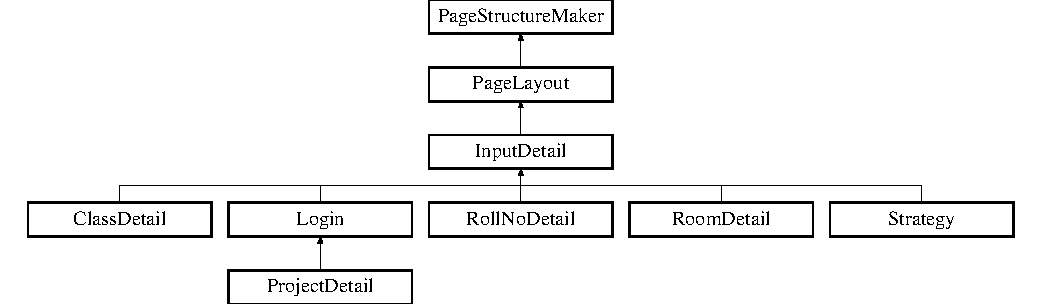
\includegraphics[height=3.000000cm]{classInputDetail}
\end{center}
\end{figure}
\subsection*{Public Member Functions}
\begin{DoxyCompactItemize}
\item 
\hyperlink{classInputDetail_ab53655b14d922eb32b5d5d06c702e497}{Input\-Detail} ()
\begin{DoxyCompactList}\small\item\em Constructor. \end{DoxyCompactList}\item 
string \hyperlink{classInputDetail_ad0a78d7c864bcccf7813a526d59573be}{Int\-To\-String} (int value)
\begin{DoxyCompactList}\small\item\em Converting integer to string. \end{DoxyCompactList}\item 
int \hyperlink{classInputDetail_aaf532dd61f0aee82b116fef2da8e821f}{String\-To\-Int} (string value)
\begin{DoxyCompactList}\small\item\em Converting String to Int. \end{DoxyCompactList}\item 
string \hyperlink{classInputDetail_a509ee6dd2de52e87cb764d0b0cceb05a}{File\-Name} (string file, string project\-I\-D, int file\-Type)
\begin{DoxyCompactList}\small\item\em For creating filename w.\-r.\-t to project\-I\-D. \end{DoxyCompactList}\item 
\hypertarget{classInputDetail_a0dbdaef0be3dc072999e4ae06f5e4e36}{\hyperlink{classInputDetail_a0dbdaef0be3dc072999e4ae06f5e4e36}{$\sim$\-Input\-Detail} ()}\label{classInputDetail_a0dbdaef0be3dc072999e4ae06f5e4e36}

\begin{DoxyCompactList}\small\item\em Destructor. \end{DoxyCompactList}\end{DoxyCompactItemize}
\subsection*{Public Attributes}
\begin{DoxyCompactItemize}
\item 
\hyperlink{classDatabase}{Database} \hyperlink{classInputDetail_ac388f27ccea9830c3c27f68d7134e061}{db}
\item 
\hyperlink{classReadInputField}{Read\-Input\-Field} \hyperlink{classInputDetail_ac0cc70b017ef94fb55acb46fc44f0df5}{read\-Field}
\end{DoxyCompactItemize}
\subsection*{Protected Attributes}
\begin{DoxyCompactItemize}
\item 
\hypertarget{classInputDetail_a2e9226db1b744de4bf406398f48cf962}{int {\bfseries i}}\label{classInputDetail_a2e9226db1b744de4bf406398f48cf962}

\item 
\hypertarget{classInputDetail_af124a26cb4e4f86d0d9eb68200ee500b}{int {\bfseries j}}\label{classInputDetail_af124a26cb4e4f86d0d9eb68200ee500b}

\item 
\hypertarget{classInputDetail_a1bb6b8bff3d5fc6d5c998e4c451035bc}{int {\bfseries k}}\label{classInputDetail_a1bb6b8bff3d5fc6d5c998e4c451035bc}

\item 
int \hyperlink{classInputDetail_a3a950727518c2f6ed3c068125a037b9e}{l}
\item 
stringstream \hyperlink{classInputDetail_a5284736b5fd3db0251cfeab7c581c0bd}{ss}
\item 
\hypertarget{classInputDetail_abacd5d7ee7ebd7e9f36bbf3fefd13a5d}{string {\bfseries temp}}\label{classInputDetail_abacd5d7ee7ebd7e9f36bbf3fefd13a5d}

\item 
string \hyperlink{classInputDetail_aa5659e496977cc83f743725f6aaf2d6a}{temp1}
\item 
\hypertarget{classInputDetail_a08069ee622c626c038b821ddcc7427b4}{string {\bfseries project\-I\-D}}\label{classInputDetail_a08069ee622c626c038b821ddcc7427b4}

\item 
\hypertarget{classInputDetail_ad3f1db4fddbe0d4efbf1d5bc74d52257}{string {\bfseries email\-I\-D}}\label{classInputDetail_ad3f1db4fddbe0d4efbf1d5bc74d52257}

\item 
string \hyperlink{classInputDetail_a4a7fb27e52bed0f40de143634f2c486b}{file\-Name}
\item 
string \hyperlink{classInputDetail_a79d8a59940f25f4d2089e241c71a4279}{where}
\item 
string \hyperlink{classInputDetail_a1abb16cd695678c3fa05e3c812823fee}{msg}
\item 
S\-T\-R\-I\-N\-G\-\_\-\-V\-E\-C \hyperlink{classInputDetail_abee6a659eb2e34b260aaf8b05d6003b4}{vec\-Temp}
\item 
S\-T\-R\-I\-N\-G\-\_\-\-V\-E\-C \hyperlink{classInputDetail_ae8ccc2e838c6d5a93ea544370dc1f272}{old\-Project}
\item 
S\-T\-R\-I\-N\-G\-\_\-\-V\-E\-C \hyperlink{classInputDetail_ab09ed4176090a72237531cedf00afb41}{split\-String}
\item 
ifstream \hyperlink{classInputDetail_a4c62c1934fbfcdcc8e2afaee44a87c15}{in\-File}
\item 
ofstream \hyperlink{classInputDetail_a2b8484cfbfee98ae69e8476f8fd40000}{out\-File}
\item 
string \hyperlink{classInputDetail_a1f276e4df260009d465032ec64f3a543}{session\-I\-D}
\end{DoxyCompactItemize}


\subsection{Detailed Description}
For declaring common variables and functions also used as base class. 

Definition at line 36 of file input\-\_\-detail.\-h.



\subsection{Constructor \& Destructor Documentation}
\hypertarget{classInputDetail_ab53655b14d922eb32b5d5d06c702e497}{\index{Input\-Detail@{Input\-Detail}!Input\-Detail@{Input\-Detail}}
\index{Input\-Detail@{Input\-Detail}!InputDetail@{Input\-Detail}}
\subsubsection[{Input\-Detail}]{\setlength{\rightskip}{0pt plus 5cm}Input\-Detail\-::\-Input\-Detail (
\begin{DoxyParamCaption}
{}
\end{DoxyParamCaption}
)}}\label{classInputDetail_ab53655b14d922eb32b5d5d06c702e497}


Constructor. 

$<$ Shortname for namespace 

Definition at line 23 of file input\-\_\-detail.\-cc.



\subsection{Member Function Documentation}
\hypertarget{classInputDetail_a509ee6dd2de52e87cb764d0b0cceb05a}{\index{Input\-Detail@{Input\-Detail}!File\-Name@{File\-Name}}
\index{File\-Name@{File\-Name}!InputDetail@{Input\-Detail}}
\subsubsection[{File\-Name}]{\setlength{\rightskip}{0pt plus 5cm}string Input\-Detail\-::\-File\-Name (
\begin{DoxyParamCaption}
\item[{string}]{file, }
\item[{string}]{project\-I\-D, }
\item[{int}]{file\-Type}
\end{DoxyParamCaption}
)}}\label{classInputDetail_a509ee6dd2de52e87cb764d0b0cceb05a}


For creating filename w.\-r.\-t to project\-I\-D. 


\begin{DoxyParams}{Parameters}
{\em project\-I\-D} & Unique I\-D i.\-e. used to read file of user \\
\hline
{\em file} & I/\-O file Name \\
\hline
{\em file\-Type} & For defining file type i.\-e I/\-P or O/\-P file. If file\-Type == 1, Input file If file\-Type == 0(else), Output File\\
\hline
\end{DoxyParams}
\begin{DoxyReturn}{Returns}
file\-Name This function will return file name with project I\-D 
\end{DoxyReturn}


Definition at line 82 of file input\-\_\-detail.\-cc.

\hypertarget{classInputDetail_ad0a78d7c864bcccf7813a526d59573be}{\index{Input\-Detail@{Input\-Detail}!Int\-To\-String@{Int\-To\-String}}
\index{Int\-To\-String@{Int\-To\-String}!InputDetail@{Input\-Detail}}
\subsubsection[{Int\-To\-String}]{\setlength{\rightskip}{0pt plus 5cm}string Input\-Detail\-::\-Int\-To\-String (
\begin{DoxyParamCaption}
\item[{int}]{value}
\end{DoxyParamCaption}
)}}\label{classInputDetail_ad0a78d7c864bcccf7813a526d59573be}


Converting integer to string. 


\begin{DoxyParams}{Parameters}
{\em value} & Value to be converted into string \\
\hline
\end{DoxyParams}


Definition at line 35 of file input\-\_\-detail.\-cc.

\hypertarget{classInputDetail_aaf532dd61f0aee82b116fef2da8e821f}{\index{Input\-Detail@{Input\-Detail}!String\-To\-Int@{String\-To\-Int}}
\index{String\-To\-Int@{String\-To\-Int}!InputDetail@{Input\-Detail}}
\subsubsection[{String\-To\-Int}]{\setlength{\rightskip}{0pt plus 5cm}int Input\-Detail\-::\-String\-To\-Int (
\begin{DoxyParamCaption}
\item[{string}]{value}
\end{DoxyParamCaption}
)}}\label{classInputDetail_aaf532dd61f0aee82b116fef2da8e821f}


Converting String to Int. 


\begin{DoxyParams}{Parameters}
{\em value} & String value to be converted into int \\
\hline
\end{DoxyParams}


Definition at line 47 of file input\-\_\-detail.\-cc.



\subsection{Member Data Documentation}
\hypertarget{classInputDetail_ac388f27ccea9830c3c27f68d7134e061}{\index{Input\-Detail@{Input\-Detail}!db@{db}}
\index{db@{db}!InputDetail@{Input\-Detail}}
\subsubsection[{db}]{\setlength{\rightskip}{0pt plus 5cm}{\bf Database} Input\-Detail\-::db}}\label{classInputDetail_ac388f27ccea9830c3c27f68d7134e061}
Data\-Base class's object 

Definition at line 67 of file input\-\_\-detail.\-h.

\hypertarget{classInputDetail_a4a7fb27e52bed0f40de143634f2c486b}{\index{Input\-Detail@{Input\-Detail}!file\-Name@{file\-Name}}
\index{file\-Name@{file\-Name}!InputDetail@{Input\-Detail}}
\subsubsection[{file\-Name}]{\setlength{\rightskip}{0pt plus 5cm}string Input\-Detail\-::file\-Name\hspace{0.3cm}{\ttfamily [protected]}}}\label{classInputDetail_a4a7fb27e52bed0f40de143634f2c486b}
File name for opening file 

Definition at line 49 of file input\-\_\-detail.\-h.

\hypertarget{classInputDetail_a4c62c1934fbfcdcc8e2afaee44a87c15}{\index{Input\-Detail@{Input\-Detail}!in\-File@{in\-File}}
\index{in\-File@{in\-File}!InputDetail@{Input\-Detail}}
\subsubsection[{in\-File}]{\setlength{\rightskip}{0pt plus 5cm}ifstream Input\-Detail\-::in\-File\hspace{0.3cm}{\ttfamily [protected]}}}\label{classInputDetail_a4c62c1934fbfcdcc8e2afaee44a87c15}
For Reading file 

Definition at line 61 of file input\-\_\-detail.\-h.

\hypertarget{classInputDetail_a3a950727518c2f6ed3c068125a037b9e}{\index{Input\-Detail@{Input\-Detail}!l@{l}}
\index{l@{l}!InputDetail@{Input\-Detail}}
\subsubsection[{l}]{\setlength{\rightskip}{0pt plus 5cm}int Input\-Detail\-::l\hspace{0.3cm}{\ttfamily [protected]}}}\label{classInputDetail_a3a950727518c2f6ed3c068125a037b9e}
Looping Variables 

Definition at line 41 of file input\-\_\-detail.\-h.

\hypertarget{classInputDetail_a1abb16cd695678c3fa05e3c812823fee}{\index{Input\-Detail@{Input\-Detail}!msg@{msg}}
\index{msg@{msg}!InputDetail@{Input\-Detail}}
\subsubsection[{msg}]{\setlength{\rightskip}{0pt plus 5cm}string Input\-Detail\-::msg\hspace{0.3cm}{\ttfamily [protected]}}}\label{classInputDetail_a1abb16cd695678c3fa05e3c812823fee}
For Displaying error message 

Definition at line 49 of file input\-\_\-detail.\-h.

\hypertarget{classInputDetail_ae8ccc2e838c6d5a93ea544370dc1f272}{\index{Input\-Detail@{Input\-Detail}!old\-Project@{old\-Project}}
\index{old\-Project@{old\-Project}!InputDetail@{Input\-Detail}}
\subsubsection[{old\-Project}]{\setlength{\rightskip}{0pt plus 5cm}S\-T\-R\-I\-N\-G\-\_\-\-V\-E\-C Input\-Detail\-::old\-Project\hspace{0.3cm}{\ttfamily [protected]}}}\label{classInputDetail_ae8ccc2e838c6d5a93ea544370dc1f272}
For stroring old projects if any 

Definition at line 55 of file input\-\_\-detail.\-h.

\hypertarget{classInputDetail_a2b8484cfbfee98ae69e8476f8fd40000}{\index{Input\-Detail@{Input\-Detail}!out\-File@{out\-File}}
\index{out\-File@{out\-File}!InputDetail@{Input\-Detail}}
\subsubsection[{out\-File}]{\setlength{\rightskip}{0pt plus 5cm}ofstream Input\-Detail\-::out\-File\hspace{0.3cm}{\ttfamily [protected]}}}\label{classInputDetail_a2b8484cfbfee98ae69e8476f8fd40000}
For writing file 

Definition at line 62 of file input\-\_\-detail.\-h.

\hypertarget{classInputDetail_ac0cc70b017ef94fb55acb46fc44f0df5}{\index{Input\-Detail@{Input\-Detail}!read\-Field@{read\-Field}}
\index{read\-Field@{read\-Field}!InputDetail@{Input\-Detail}}
\subsubsection[{read\-Field}]{\setlength{\rightskip}{0pt plus 5cm}{\bf Read\-Input\-Field} Input\-Detail\-::read\-Field}}\label{classInputDetail_ac0cc70b017ef94fb55acb46fc44f0df5}
Reading Inpur fields 

Definition at line 68 of file input\-\_\-detail.\-h.

\hypertarget{classInputDetail_a1f276e4df260009d465032ec64f3a543}{\index{Input\-Detail@{Input\-Detail}!session\-I\-D@{session\-I\-D}}
\index{session\-I\-D@{session\-I\-D}!InputDetail@{Input\-Detail}}
\subsubsection[{session\-I\-D}]{\setlength{\rightskip}{0pt plus 5cm}string Input\-Detail\-::session\-I\-D\hspace{0.3cm}{\ttfamily [protected]}}}\label{classInputDetail_a1f276e4df260009d465032ec64f3a543}
Session I\-D 

Definition at line 63 of file input\-\_\-detail.\-h.

\hypertarget{classInputDetail_ab09ed4176090a72237531cedf00afb41}{\index{Input\-Detail@{Input\-Detail}!split\-String@{split\-String}}
\index{split\-String@{split\-String}!InputDetail@{Input\-Detail}}
\subsubsection[{split\-String}]{\setlength{\rightskip}{0pt plus 5cm}S\-T\-R\-I\-N\-G\-\_\-\-V\-E\-C Input\-Detail\-::split\-String\hspace{0.3cm}{\ttfamily [protected]}}}\label{classInputDetail_ab09ed4176090a72237531cedf00afb41}
For storing values of splitted string 

Definition at line 55 of file input\-\_\-detail.\-h.

\hypertarget{classInputDetail_a5284736b5fd3db0251cfeab7c581c0bd}{\index{Input\-Detail@{Input\-Detail}!ss@{ss}}
\index{ss@{ss}!InputDetail@{Input\-Detail}}
\subsubsection[{ss}]{\setlength{\rightskip}{0pt plus 5cm}stringstream Input\-Detail\-::ss\hspace{0.3cm}{\ttfamily [protected]}}}\label{classInputDetail_a5284736b5fd3db0251cfeab7c581c0bd}
For converting int to string 

Definition at line 43 of file input\-\_\-detail.\-h.

\hypertarget{classInputDetail_aa5659e496977cc83f743725f6aaf2d6a}{\index{Input\-Detail@{Input\-Detail}!temp1@{temp1}}
\index{temp1@{temp1}!InputDetail@{Input\-Detail}}
\subsubsection[{temp1}]{\setlength{\rightskip}{0pt plus 5cm}string Input\-Detail\-::temp1\hspace{0.3cm}{\ttfamily [protected]}}}\label{classInputDetail_aa5659e496977cc83f743725f6aaf2d6a}
For temporary strorage 

Definition at line 44 of file input\-\_\-detail.\-h.

\hypertarget{classInputDetail_abee6a659eb2e34b260aaf8b05d6003b4}{\index{Input\-Detail@{Input\-Detail}!vec\-Temp@{vec\-Temp}}
\index{vec\-Temp@{vec\-Temp}!InputDetail@{Input\-Detail}}
\subsubsection[{vec\-Temp}]{\setlength{\rightskip}{0pt plus 5cm}S\-T\-R\-I\-N\-G\-\_\-\-V\-E\-C Input\-Detail\-::vec\-Temp\hspace{0.3cm}{\ttfamily [protected]}}}\label{classInputDetail_abee6a659eb2e34b260aaf8b05d6003b4}
string Vector temporary use 

Definition at line 55 of file input\-\_\-detail.\-h.

\hypertarget{classInputDetail_a79d8a59940f25f4d2089e241c71a4279}{\index{Input\-Detail@{Input\-Detail}!where@{where}}
\index{where@{where}!InputDetail@{Input\-Detail}}
\subsubsection[{where}]{\setlength{\rightskip}{0pt plus 5cm}string Input\-Detail\-::where\hspace{0.3cm}{\ttfamily [protected]}}}\label{classInputDetail_a79d8a59940f25f4d2089e241c71a4279}
Temp variable to store where clause 

Definition at line 49 of file input\-\_\-detail.\-h.



The documentation for this class was generated from the following files\-:\begin{DoxyCompactItemize}
\item 
src/cpp/frontend/header/input\-\_\-detail.\-h\item 
src/cpp/frontend/\hyperlink{input__detail_8cc}{input\-\_\-detail.\-cc}\end{DoxyCompactItemize}

\hypertarget{classInputFieldName}{\section{\-Input\-Field\-Name \-Class \-Reference}
\label{classInputFieldName}\index{\-Input\-Field\-Name@{\-Input\-Field\-Name}}
}


{\ttfamily \#include $<$inputfieldname.\-h$>$}

\subsection*{\-Public \-Member \-Functions}
\begin{DoxyCompactItemize}
\item 
\hyperlink{classInputFieldName_a185ace189c56eed847111756922e5158}{\-Input\-Field\-Name} ()
\item 
void \hyperlink{classInputFieldName_a5232eb098c6354207a97264cbc14a3fa}{\-Set\-Field\-Names} ()
\end{DoxyCompactItemize}
\subsection*{\-Public \-Attributes}
\begin{DoxyCompactItemize}
\item 
string \hyperlink{classInputFieldName_ad8b28ebeabdabb5967542e317f549280}{class\-Name}
\item 
string \hyperlink{classInputFieldName_a5bf413dee6dcf29c1872e93f150d48c0}{total\-Classes}
\item 
string \hyperlink{classInputFieldName_ac58130077f39d82aaf447b1a67e9f70f}{total\-Subjects}
\item 
string \hyperlink{classInputFieldName_af1cc6871c33344c365e6e25ea482bd48}{subject\-Code}
\item 
string \hyperlink{classInputFieldName_a0614731b959afef6bb00f9fc957e7521}{subject\-Name}
\item 
string \hyperlink{classInputFieldName_a6a67c361f3b631fb6c3620c14a615fb9}{class\-I\-D}
\item 
string \hyperlink{classInputFieldName_a161d155f8faca2c5dea1bbd607b17553}{prefix}
\item 
string \hyperlink{classInputFieldName_a24baf5c915b4ee0fb8678e03adec043a}{start\-Roll\-No}
\item 
string \hyperlink{classInputFieldName_a06435f9ba5a529cbba4ee1ce9b02e5cc}{end\-Roll\-No}
\item 
string \hyperlink{classInputFieldName_a9ee6ee84737e1199bdfd9fb24c82c2c7}{not\-Included}
\item 
string \hyperlink{classInputFieldName_ab93b034743570810afe89aea88a7bbf6}{project\-Name}
\item 
string \hyperlink{classInputFieldName_ac4bd117f3137956473f1a1d5ce9106a5}{project\-I\-D}
\item 
string \hyperlink{classInputFieldName_aaa398a603dfe98f4eca022ec9d90bc09}{project\-Type}
\item 
string \hyperlink{classInputFieldName_a05541618feaaebe7a3f74b0bf8fa74b9}{email\-I\-D}
\item 
string \hyperlink{classInputFieldName_a318f819ef4663d7e5f40d91180093cb9}{password}
\item 
string \hyperlink{classInputFieldName_acd50095ae8540a735bcd5787b904b06c}{retype\-Password}
\item 
string \hyperlink{classInputFieldName_a26cffcb455cb1b977aa60b68c5b48fe4}{key}
\item 
string \hyperlink{classInputFieldName_af88ac102ec3a4adbb9edc7c3d61919cb}{total\-Centres}
\item 
string \hyperlink{classInputFieldName_a51fe8230341d7863ffd4672f2c986beb}{total\-Rooms}
\item 
string \hyperlink{classInputFieldName_a19c67f2d38cde97f856d4ca3639f4fc7}{centre\-Name}
\item 
string \hyperlink{classInputFieldName_abb6b245e03e76aa29d7ef8733298e72f}{room\-No}
\item 
string \hyperlink{classInputFieldName_a1b5a819437f52b4bb6b0ea59f542f9a9}{rows}
\item 
string \hyperlink{classInputFieldName_abca049f347e589f24b672c19907c5c72}{columns}
\item 
string \hyperlink{classInputFieldName_a9a6b827d404cb279cc0ed836c069e4a9}{strategy\-Choice}
\item 
string \hyperlink{classInputFieldName_a4cee41667cdc0e38f8f76af94ef39c36}{exam\-Name}
\item 
string \hyperlink{classInputFieldName_a4e60d793497c36b2d80e2411cbb915d8}{exam\-Date}
\item 
string \hyperlink{classInputFieldName_afef45e787d3c737f9bdc3126ce29d8b9}{exam\-Session}
\item 
string \hyperlink{classInputFieldName_ab667062be019e5912683d33c45885bd3}{exam\-Time}
\item 
string \hyperlink{classInputFieldName_affaa2fe8246959748f43ea58f161b2b5}{exam\-Venue}
\item 
string \hyperlink{classInputFieldName_afb053a44abe76e108533e23902e90321}{date}
\item 
string \hyperlink{classInputFieldName_a3cc09a852d20e96bb4908b9f66c01ed7}{exam\-Code}
\item 
string \hyperlink{classInputFieldName_a12ba65660edd7f8f7ecf1e25893716da}{total\-Days}
\item 
string \hyperlink{classInputFieldName_a6de91205e7eac3168e17d100ab4d8e64}{same\-Detail}
\item 
string \hyperlink{classInputFieldName_a12e0f0ec0ad7962271d6dae576e5ee0a}{last\-Row}
\item 
string \hyperlink{classInputFieldName_adfb1d136313267eecabe30391a03b49b}{row\-Index}
\end{DoxyCompactItemize}


\subsection{\-Detailed \-Description}
-\/-\/-\/-\/-\/-\/-\/-\/-\/-\/-\/-\/-\/-\/-\/-\/-\/-\/-\/-\/-\/-\/-\/-\/-\/-\/-\/-\/-\/-\/-\/-\/-\/-\/-\/-\/-\/-\/-\/-\/-\/-\/-\/-\/-\/-\/-\/-\/-\/-\/-\/-\/-\/-\/-\/-\/-\/-\/-\/-\/-\/-\/-\/-\/-\/-\/-\/ \-Include local header file that has global header files -\/-\/-\/-\/-\/-\/-\/-\/-\/-\/-\/-\/-\/-\/-\/-\/-\/-\/-\/-\/-\/-\/-\/-\/-\/-\/-\/-\/-\/-\/-\/-\/-\/-\/-\/-\/-\/-\/-\/-\/-\/-\/-\/-\/-\/-\/-\/-\/-\/-\/-\/-\/-\/-\/-\/-\/-\/-\/-\/-\/-\/-\/-\/-\/-\/-\/ =================================================================== \-Class\-: \hyperlink{classInputFieldName}{\-Input\-Field\-Name} \-Description\-: \-This class has variable names for all fields that are used to take input from user. =================================================================== 

\-Definition at line 37 of file inputfieldname.\-h.



\subsection{\-Constructor \& \-Destructor \-Documentation}
\hypertarget{classInputFieldName_a185ace189c56eed847111756922e5158}{\index{\-Input\-Field\-Name@{\-Input\-Field\-Name}!\-Input\-Field\-Name@{\-Input\-Field\-Name}}
\index{\-Input\-Field\-Name@{\-Input\-Field\-Name}!InputFieldName@{\-Input\-Field\-Name}}
\subsubsection[{\-Input\-Field\-Name}]{\setlength{\rightskip}{0pt plus 5cm}{\bf \-Input\-Field\-Name\-::\-Input\-Field\-Name} (
\begin{DoxyParamCaption}
{}
\end{DoxyParamCaption}
)}}\label{classInputFieldName_a185ace189c56eed847111756922e5158}
\-Constructor

-\/-\/-\/-\/-\/-\/-\/-\/-\/-\/-\/-\/-\/-\/-\/-\/-\/-\/-\/-\/-\/-\/-\/-\/-\/-\/-\/-\/-\/-\/-\/-\/-\/-\/-\/-\/-\/-\/-\/-\/-\/-\/-\/-\/-\/-\/-\/-\/-\/-\/-\/-\/-\/-\/-\/-\/-\/-\/-\/-\/-\/-\/-\/-\/-\/-\/-\/ \-Include header file that contains \hyperlink{classInputFieldName}{\-Input\-Field\-Name} \-Class's \-Declaration -\/-\/-\/-\/-\/-\/-\/-\/-\/-\/-\/-\/-\/-\/-\/-\/-\/-\/-\/-\/-\/-\/-\/-\/-\/-\/-\/-\/-\/-\/-\/-\/-\/-\/-\/-\/-\/-\/-\/-\/-\/-\/-\/-\/-\/-\/-\/-\/-\/-\/-\/-\/-\/-\/-\/-\/-\/-\/-\/-\/-\/-\/-\/-\/-\/-\/ -\/-\/-\/-\/-\/-\/-\/-\/-\/-\/-\/-\/-\/-\/-\/-\/-\/-\/-\/-\/-\/-\/-\/-\/-\/-\/-\/-\/-\/-\/-\/-\/-\/-\/-\/-\/-\/-\/-\/-\/-\/-\/-\/-\/-\/-\/-\/-\/-\/-\/-\/-\/-\/-\/-\/-\/-\/-\/-\/-\/-\/-\/-\/-\/-\/-\/-\/ \-Definition of member functions -\/-\/-\/-\/-\/-\/-\/-\/-\/-\/-\/-\/-\/-\/-\/-\/-\/-\/-\/-\/-\/-\/-\/-\/-\/-\/-\/-\/-\/-\/-\/-\/-\/-\/-\/-\/-\/-\/-\/-\/-\/-\/-\/-\/-\/-\/-\/-\/-\/-\/-\/-\/-\/-\/-\/-\/-\/-\/-\/-\/-\/-\/-\/-\/-\/-\/ -\/-\/-\/-\/-\/-\/-\/-\/-\/-\/-\/-\/-\/-\/-\/-\/-\/-\/-\/-\/-\/-\/-\/-\/-\/-\/-\/-\/-\/-\/-\/-\/-\/-\/-\/-\/-\/-\/-\/-\/-\/-\/-\/-\/-\/-\/-\/-\/-\/-\/-\/-\/-\/-\/-\/-\/-\/-\/-\/-\/-\/-\/-\/-\/-\/-\/-\/-\/ \-Class\-: \hyperlink{classInputFieldName}{\-Input\-Field\-Name} \-Method\-: \hyperlink{classInputFieldName}{\-Input\-Field\-Name} \-:\-: \hyperlink{classInputFieldName_a185ace189c56eed847111756922e5158}{\-Input\-Field\-Name()} \-Description\-: \-Constructor calls \hyperlink{classInputFieldName_a5232eb098c6354207a97264cbc14a3fa}{\-Set\-Field\-Names()} -\/-\/-\/-\/-\/-\/-\/-\/-\/-\/-\/-\/-\/-\/-\/-\/-\/-\/-\/-\/-\/-\/-\/-\/-\/-\/-\/-\/-\/-\/-\/-\/-\/-\/-\/-\/-\/-\/-\/-\/-\/-\/-\/-\/-\/-\/-\/-\/-\/-\/-\/-\/-\/-\/-\/-\/-\/-\/-\/-\/-\/-\/-\/-\/-\/-\/-\/-\/ 

\-Definition at line 38 of file inputfieldname.\-cc.



\subsection{\-Member \-Function \-Documentation}
\hypertarget{classInputFieldName_a5232eb098c6354207a97264cbc14a3fa}{\index{\-Input\-Field\-Name@{\-Input\-Field\-Name}!\-Set\-Field\-Names@{\-Set\-Field\-Names}}
\index{\-Set\-Field\-Names@{\-Set\-Field\-Names}!InputFieldName@{\-Input\-Field\-Name}}
\subsubsection[{\-Set\-Field\-Names}]{\setlength{\rightskip}{0pt plus 5cm}void {\bf \-Input\-Field\-Name\-::\-Set\-Field\-Names} (
\begin{DoxyParamCaption}
{}
\end{DoxyParamCaption}
)}}\label{classInputFieldName_a5232eb098c6354207a97264cbc14a3fa}
\-Set \-Field \-Values

-\/-\/-\/-\/-\/-\/-\/-\/-\/-\/-\/-\/-\/-\/-\/-\/-\/-\/-\/-\/-\/-\/-\/-\/-\/-\/-\/-\/-\/-\/-\/-\/-\/-\/-\/-\/-\/-\/-\/-\/-\/-\/-\/-\/-\/-\/-\/-\/-\/-\/-\/-\/-\/-\/-\/-\/-\/-\/-\/-\/-\/-\/-\/-\/-\/-\/-\/-\/ \-Class\-: \hyperlink{classInputFieldName}{\-Input\-Field\-Name} \-Method\-: \hyperlink{classInputFieldName}{\-Input\-Field\-Name} \-:\-: \hyperlink{classInputFieldName_a5232eb098c6354207a97264cbc14a3fa}{\-Set\-Field\-Names()} \-Description\-: \-Assign \-Values of field names in its respective variables. -\/-\/-\/-\/-\/-\/-\/-\/-\/-\/-\/-\/-\/-\/-\/-\/-\/-\/-\/-\/-\/-\/-\/-\/-\/-\/-\/-\/-\/-\/-\/-\/-\/-\/-\/-\/-\/-\/-\/-\/-\/-\/-\/-\/-\/-\/-\/-\/-\/-\/-\/-\/-\/-\/-\/-\/-\/-\/-\/-\/-\/-\/-\/-\/-\/-\/-\/-\/ 

\-Definition at line 52 of file inputfieldname.\-cc.



\subsection{\-Member \-Data \-Documentation}
\hypertarget{classInputFieldName_a19c67f2d38cde97f856d4ca3639f4fc7}{\index{\-Input\-Field\-Name@{\-Input\-Field\-Name}!centre\-Name@{centre\-Name}}
\index{centre\-Name@{centre\-Name}!InputFieldName@{\-Input\-Field\-Name}}
\subsubsection[{centre\-Name}]{\setlength{\rightskip}{0pt plus 5cm}string {\bf \-Input\-Field\-Name\-::centre\-Name}}}\label{classInputFieldName_a19c67f2d38cde97f856d4ca3639f4fc7}
\-Center \-Name 

\-Definition at line 63 of file inputfieldname.\-h.

\hypertarget{classInputFieldName_a6a67c361f3b631fb6c3620c14a615fb9}{\index{\-Input\-Field\-Name@{\-Input\-Field\-Name}!class\-I\-D@{class\-I\-D}}
\index{class\-I\-D@{class\-I\-D}!InputFieldName@{\-Input\-Field\-Name}}
\subsubsection[{class\-I\-D}]{\setlength{\rightskip}{0pt plus 5cm}string {\bf \-Input\-Field\-Name\-::class\-I\-D}}}\label{classInputFieldName_a6a67c361f3b631fb6c3620c14a615fb9}
\-Class id 

\-Definition at line 44 of file inputfieldname.\-h.

\hypertarget{classInputFieldName_ad8b28ebeabdabb5967542e317f549280}{\index{\-Input\-Field\-Name@{\-Input\-Field\-Name}!class\-Name@{class\-Name}}
\index{class\-Name@{class\-Name}!InputFieldName@{\-Input\-Field\-Name}}
\subsubsection[{class\-Name}]{\setlength{\rightskip}{0pt plus 5cm}string {\bf \-Input\-Field\-Name\-::class\-Name}}}\label{classInputFieldName_ad8b28ebeabdabb5967542e317f549280}
\-Class\-Name 

\-Definition at line 44 of file inputfieldname.\-h.

\hypertarget{classInputFieldName_abca049f347e589f24b672c19907c5c72}{\index{\-Input\-Field\-Name@{\-Input\-Field\-Name}!columns@{columns}}
\index{columns@{columns}!InputFieldName@{\-Input\-Field\-Name}}
\subsubsection[{columns}]{\setlength{\rightskip}{0pt plus 5cm}string {\bf \-Input\-Field\-Name\-::columns}}}\label{classInputFieldName_abca049f347e589f24b672c19907c5c72}
\-Columns in room 

\-Definition at line 63 of file inputfieldname.\-h.

\hypertarget{classInputFieldName_afb053a44abe76e108533e23902e90321}{\index{\-Input\-Field\-Name@{\-Input\-Field\-Name}!date@{date}}
\index{date@{date}!InputFieldName@{\-Input\-Field\-Name}}
\subsubsection[{date}]{\setlength{\rightskip}{0pt plus 5cm}string {\bf \-Input\-Field\-Name\-::date}}}\label{classInputFieldName_afb053a44abe76e108533e23902e90321}
\-Date of examination 

\-Definition at line 63 of file inputfieldname.\-h.

\hypertarget{classInputFieldName_a05541618feaaebe7a3f74b0bf8fa74b9}{\index{\-Input\-Field\-Name@{\-Input\-Field\-Name}!email\-I\-D@{email\-I\-D}}
\index{email\-I\-D@{email\-I\-D}!InputFieldName@{\-Input\-Field\-Name}}
\subsubsection[{email\-I\-D}]{\setlength{\rightskip}{0pt plus 5cm}string {\bf \-Input\-Field\-Name\-::email\-I\-D}}}\label{classInputFieldName_a05541618feaaebe7a3f74b0bf8fa74b9}
\-Email \-Field 

\-Definition at line 63 of file inputfieldname.\-h.

\hypertarget{classInputFieldName_a06435f9ba5a529cbba4ee1ce9b02e5cc}{\index{\-Input\-Field\-Name@{\-Input\-Field\-Name}!end\-Roll\-No@{end\-Roll\-No}}
\index{end\-Roll\-No@{end\-Roll\-No}!InputFieldName@{\-Input\-Field\-Name}}
\subsubsection[{end\-Roll\-No}]{\setlength{\rightskip}{0pt plus 5cm}string {\bf \-Input\-Field\-Name\-::end\-Roll\-No}}}\label{classInputFieldName_a06435f9ba5a529cbba4ee1ce9b02e5cc}
ending rollno 

\-Definition at line 44 of file inputfieldname.\-h.

\hypertarget{classInputFieldName_a3cc09a852d20e96bb4908b9f66c01ed7}{\index{\-Input\-Field\-Name@{\-Input\-Field\-Name}!exam\-Code@{exam\-Code}}
\index{exam\-Code@{exam\-Code}!InputFieldName@{\-Input\-Field\-Name}}
\subsubsection[{exam\-Code}]{\setlength{\rightskip}{0pt plus 5cm}string {\bf \-Input\-Field\-Name\-::exam\-Code}}}\label{classInputFieldName_a3cc09a852d20e96bb4908b9f66c01ed7}
\-Exam code accord to date sheet 

\-Definition at line 63 of file inputfieldname.\-h.

\hypertarget{classInputFieldName_a4e60d793497c36b2d80e2411cbb915d8}{\index{\-Input\-Field\-Name@{\-Input\-Field\-Name}!exam\-Date@{exam\-Date}}
\index{exam\-Date@{exam\-Date}!InputFieldName@{\-Input\-Field\-Name}}
\subsubsection[{exam\-Date}]{\setlength{\rightskip}{0pt plus 5cm}string {\bf \-Input\-Field\-Name\-::exam\-Date}}}\label{classInputFieldName_a4e60d793497c36b2d80e2411cbb915d8}
\-Examination \-Date 

\-Definition at line 63 of file inputfieldname.\-h.

\hypertarget{classInputFieldName_a4cee41667cdc0e38f8f76af94ef39c36}{\index{\-Input\-Field\-Name@{\-Input\-Field\-Name}!exam\-Name@{exam\-Name}}
\index{exam\-Name@{exam\-Name}!InputFieldName@{\-Input\-Field\-Name}}
\subsubsection[{exam\-Name}]{\setlength{\rightskip}{0pt plus 5cm}string {\bf \-Input\-Field\-Name\-::exam\-Name}}}\label{classInputFieldName_a4cee41667cdc0e38f8f76af94ef39c36}
\-Examination \-Name 

\-Definition at line 63 of file inputfieldname.\-h.

\hypertarget{classInputFieldName_afef45e787d3c737f9bdc3126ce29d8b9}{\index{\-Input\-Field\-Name@{\-Input\-Field\-Name}!exam\-Session@{exam\-Session}}
\index{exam\-Session@{exam\-Session}!InputFieldName@{\-Input\-Field\-Name}}
\subsubsection[{exam\-Session}]{\setlength{\rightskip}{0pt plus 5cm}string {\bf \-Input\-Field\-Name\-::exam\-Session}}}\label{classInputFieldName_afef45e787d3c737f9bdc3126ce29d8b9}
\-Exam. \-Session (\-M/\-E) 

\-Definition at line 63 of file inputfieldname.\-h.

\hypertarget{classInputFieldName_ab667062be019e5912683d33c45885bd3}{\index{\-Input\-Field\-Name@{\-Input\-Field\-Name}!exam\-Time@{exam\-Time}}
\index{exam\-Time@{exam\-Time}!InputFieldName@{\-Input\-Field\-Name}}
\subsubsection[{exam\-Time}]{\setlength{\rightskip}{0pt plus 5cm}string {\bf \-Input\-Field\-Name\-::exam\-Time}}}\label{classInputFieldName_ab667062be019e5912683d33c45885bd3}
\-Examination \-Time 

\-Definition at line 63 of file inputfieldname.\-h.

\hypertarget{classInputFieldName_affaa2fe8246959748f43ea58f161b2b5}{\index{\-Input\-Field\-Name@{\-Input\-Field\-Name}!exam\-Venue@{exam\-Venue}}
\index{exam\-Venue@{exam\-Venue}!InputFieldName@{\-Input\-Field\-Name}}
\subsubsection[{exam\-Venue}]{\setlength{\rightskip}{0pt plus 5cm}string {\bf \-Input\-Field\-Name\-::exam\-Venue}}}\label{classInputFieldName_affaa2fe8246959748f43ea58f161b2b5}
\-Examination \-Venue 

\-Definition at line 63 of file inputfieldname.\-h.

\hypertarget{classInputFieldName_a26cffcb455cb1b977aa60b68c5b48fe4}{\index{\-Input\-Field\-Name@{\-Input\-Field\-Name}!key@{key}}
\index{key@{key}!InputFieldName@{\-Input\-Field\-Name}}
\subsubsection[{key}]{\setlength{\rightskip}{0pt plus 5cm}string {\bf \-Input\-Field\-Name\-::key}}}\label{classInputFieldName_a26cffcb455cb1b977aa60b68c5b48fe4}
\-Registration \-Key 

\-Definition at line 63 of file inputfieldname.\-h.

\hypertarget{classInputFieldName_a12e0f0ec0ad7962271d6dae576e5ee0a}{\index{\-Input\-Field\-Name@{\-Input\-Field\-Name}!last\-Row@{last\-Row}}
\index{last\-Row@{last\-Row}!InputFieldName@{\-Input\-Field\-Name}}
\subsubsection[{last\-Row}]{\setlength{\rightskip}{0pt plus 5cm}string {\bf \-Input\-Field\-Name\-::last\-Row}}}\label{classInputFieldName_a12e0f0ec0ad7962271d6dae576e5ee0a}
\-Last row index value 

\-Definition at line 63 of file inputfieldname.\-h.

\hypertarget{classInputFieldName_a9ee6ee84737e1199bdfd9fb24c82c2c7}{\index{\-Input\-Field\-Name@{\-Input\-Field\-Name}!not\-Included@{not\-Included}}
\index{not\-Included@{not\-Included}!InputFieldName@{\-Input\-Field\-Name}}
\subsubsection[{not\-Included}]{\setlength{\rightskip}{0pt plus 5cm}string {\bf \-Input\-Field\-Name\-::not\-Included}}}\label{classInputFieldName_a9ee6ee84737e1199bdfd9fb24c82c2c7}
roll that are not included in seating plan 

\-Definition at line 44 of file inputfieldname.\-h.

\hypertarget{classInputFieldName_a318f819ef4663d7e5f40d91180093cb9}{\index{\-Input\-Field\-Name@{\-Input\-Field\-Name}!password@{password}}
\index{password@{password}!InputFieldName@{\-Input\-Field\-Name}}
\subsubsection[{password}]{\setlength{\rightskip}{0pt plus 5cm}string {\bf \-Input\-Field\-Name\-::password}}}\label{classInputFieldName_a318f819ef4663d7e5f40d91180093cb9}
\-Password field 

\-Definition at line 63 of file inputfieldname.\-h.

\hypertarget{classInputFieldName_a161d155f8faca2c5dea1bbd607b17553}{\index{\-Input\-Field\-Name@{\-Input\-Field\-Name}!prefix@{prefix}}
\index{prefix@{prefix}!InputFieldName@{\-Input\-Field\-Name}}
\subsubsection[{prefix}]{\setlength{\rightskip}{0pt plus 5cm}string {\bf \-Input\-Field\-Name\-::prefix}}}\label{classInputFieldName_a161d155f8faca2c5dea1bbd607b17553}
\-Prefix of rollno 

\-Definition at line 44 of file inputfieldname.\-h.

\hypertarget{classInputFieldName_ac4bd117f3137956473f1a1d5ce9106a5}{\index{\-Input\-Field\-Name@{\-Input\-Field\-Name}!project\-I\-D@{project\-I\-D}}
\index{project\-I\-D@{project\-I\-D}!InputFieldName@{\-Input\-Field\-Name}}
\subsubsection[{project\-I\-D}]{\setlength{\rightskip}{0pt plus 5cm}string {\bf \-Input\-Field\-Name\-::project\-I\-D}}}\label{classInputFieldName_ac4bd117f3137956473f1a1d5ce9106a5}
\-Project \-I\-D 

\-Definition at line 44 of file inputfieldname.\-h.

\hypertarget{classInputFieldName_ab93b034743570810afe89aea88a7bbf6}{\index{\-Input\-Field\-Name@{\-Input\-Field\-Name}!project\-Name@{project\-Name}}
\index{project\-Name@{project\-Name}!InputFieldName@{\-Input\-Field\-Name}}
\subsubsection[{project\-Name}]{\setlength{\rightskip}{0pt plus 5cm}string {\bf \-Input\-Field\-Name\-::project\-Name}}}\label{classInputFieldName_ab93b034743570810afe89aea88a7bbf6}
\-Project \-Name 

\-Definition at line 44 of file inputfieldname.\-h.

\hypertarget{classInputFieldName_aaa398a603dfe98f4eca022ec9d90bc09}{\index{\-Input\-Field\-Name@{\-Input\-Field\-Name}!project\-Type@{project\-Type}}
\index{project\-Type@{project\-Type}!InputFieldName@{\-Input\-Field\-Name}}
\subsubsection[{project\-Type}]{\setlength{\rightskip}{0pt plus 5cm}string {\bf \-Input\-Field\-Name\-::project\-Type}}}\label{classInputFieldName_aaa398a603dfe98f4eca022ec9d90bc09}
\-Project\-Type ie new or old 

\-Definition at line 44 of file inputfieldname.\-h.

\hypertarget{classInputFieldName_acd50095ae8540a735bcd5787b904b06c}{\index{\-Input\-Field\-Name@{\-Input\-Field\-Name}!retype\-Password@{retype\-Password}}
\index{retype\-Password@{retype\-Password}!InputFieldName@{\-Input\-Field\-Name}}
\subsubsection[{retype\-Password}]{\setlength{\rightskip}{0pt plus 5cm}string {\bf \-Input\-Field\-Name\-::retype\-Password}}}\label{classInputFieldName_acd50095ae8540a735bcd5787b904b06c}
\-Retype \-Password 

\-Definition at line 63 of file inputfieldname.\-h.

\hypertarget{classInputFieldName_abb6b245e03e76aa29d7ef8733298e72f}{\index{\-Input\-Field\-Name@{\-Input\-Field\-Name}!room\-No@{room\-No}}
\index{room\-No@{room\-No}!InputFieldName@{\-Input\-Field\-Name}}
\subsubsection[{room\-No}]{\setlength{\rightskip}{0pt plus 5cm}string {\bf \-Input\-Field\-Name\-::room\-No}}}\label{classInputFieldName_abb6b245e03e76aa29d7ef8733298e72f}
\-Room \-Nos w.\-r.\-t to centre name 

\-Definition at line 63 of file inputfieldname.\-h.

\hypertarget{classInputFieldName_adfb1d136313267eecabe30391a03b49b}{\index{\-Input\-Field\-Name@{\-Input\-Field\-Name}!row\-Index@{row\-Index}}
\index{row\-Index@{row\-Index}!InputFieldName@{\-Input\-Field\-Name}}
\subsubsection[{row\-Index}]{\setlength{\rightskip}{0pt plus 5cm}string {\bf \-Input\-Field\-Name\-::row\-Index}}}\label{classInputFieldName_adfb1d136313267eecabe30391a03b49b}
\-Index values of all rows 

\-Definition at line 63 of file inputfieldname.\-h.

\hypertarget{classInputFieldName_a1b5a819437f52b4bb6b0ea59f542f9a9}{\index{\-Input\-Field\-Name@{\-Input\-Field\-Name}!rows@{rows}}
\index{rows@{rows}!InputFieldName@{\-Input\-Field\-Name}}
\subsubsection[{rows}]{\setlength{\rightskip}{0pt plus 5cm}string {\bf \-Input\-Field\-Name\-::rows}}}\label{classInputFieldName_a1b5a819437f52b4bb6b0ea59f542f9a9}
\-Rows of room 

\-Definition at line 63 of file inputfieldname.\-h.

\hypertarget{classInputFieldName_a6de91205e7eac3168e17d100ab4d8e64}{\index{\-Input\-Field\-Name@{\-Input\-Field\-Name}!same\-Detail@{same\-Detail}}
\index{same\-Detail@{same\-Detail}!InputFieldName@{\-Input\-Field\-Name}}
\subsubsection[{same\-Detail}]{\setlength{\rightskip}{0pt plus 5cm}string {\bf \-Input\-Field\-Name\-::same\-Detail}}}\label{classInputFieldName_a6de91205e7eac3168e17d100ab4d8e64}
\-Same detail of room, exam, strategy for seating plan 

\-Definition at line 63 of file inputfieldname.\-h.

\hypertarget{classInputFieldName_a24baf5c915b4ee0fb8678e03adec043a}{\index{\-Input\-Field\-Name@{\-Input\-Field\-Name}!start\-Roll\-No@{start\-Roll\-No}}
\index{start\-Roll\-No@{start\-Roll\-No}!InputFieldName@{\-Input\-Field\-Name}}
\subsubsection[{start\-Roll\-No}]{\setlength{\rightskip}{0pt plus 5cm}string {\bf \-Input\-Field\-Name\-::start\-Roll\-No}}}\label{classInputFieldName_a24baf5c915b4ee0fb8678e03adec043a}
starting roll no 

\-Definition at line 44 of file inputfieldname.\-h.

\hypertarget{classInputFieldName_a9a6b827d404cb279cc0ed836c069e4a9}{\index{\-Input\-Field\-Name@{\-Input\-Field\-Name}!strategy\-Choice@{strategy\-Choice}}
\index{strategy\-Choice@{strategy\-Choice}!InputFieldName@{\-Input\-Field\-Name}}
\subsubsection[{strategy\-Choice}]{\setlength{\rightskip}{0pt plus 5cm}string {\bf \-Input\-Field\-Name\-::strategy\-Choice}}}\label{classInputFieldName_a9a6b827d404cb279cc0ed836c069e4a9}
\hyperlink{classStrategy}{\-Strategy} option selected by user 

\-Definition at line 63 of file inputfieldname.\-h.

\hypertarget{classInputFieldName_af1cc6871c33344c365e6e25ea482bd48}{\index{\-Input\-Field\-Name@{\-Input\-Field\-Name}!subject\-Code@{subject\-Code}}
\index{subject\-Code@{subject\-Code}!InputFieldName@{\-Input\-Field\-Name}}
\subsubsection[{subject\-Code}]{\setlength{\rightskip}{0pt plus 5cm}string {\bf \-Input\-Field\-Name\-::subject\-Code}}}\label{classInputFieldName_af1cc6871c33344c365e6e25ea482bd48}
\-Subject\-Code 

\-Definition at line 44 of file inputfieldname.\-h.

\hypertarget{classInputFieldName_a0614731b959afef6bb00f9fc957e7521}{\index{\-Input\-Field\-Name@{\-Input\-Field\-Name}!subject\-Name@{subject\-Name}}
\index{subject\-Name@{subject\-Name}!InputFieldName@{\-Input\-Field\-Name}}
\subsubsection[{subject\-Name}]{\setlength{\rightskip}{0pt plus 5cm}string {\bf \-Input\-Field\-Name\-::subject\-Name}}}\label{classInputFieldName_a0614731b959afef6bb00f9fc957e7521}
\-Subject\-Name 

\-Definition at line 44 of file inputfieldname.\-h.

\hypertarget{classInputFieldName_af88ac102ec3a4adbb9edc7c3d61919cb}{\index{\-Input\-Field\-Name@{\-Input\-Field\-Name}!total\-Centres@{total\-Centres}}
\index{total\-Centres@{total\-Centres}!InputFieldName@{\-Input\-Field\-Name}}
\subsubsection[{total\-Centres}]{\setlength{\rightskip}{0pt plus 5cm}string {\bf \-Input\-Field\-Name\-::total\-Centres}}}\label{classInputFieldName_af88ac102ec3a4adbb9edc7c3d61919cb}
\-Total centres 

\-Definition at line 63 of file inputfieldname.\-h.

\hypertarget{classInputFieldName_a5bf413dee6dcf29c1872e93f150d48c0}{\index{\-Input\-Field\-Name@{\-Input\-Field\-Name}!total\-Classes@{total\-Classes}}
\index{total\-Classes@{total\-Classes}!InputFieldName@{\-Input\-Field\-Name}}
\subsubsection[{total\-Classes}]{\setlength{\rightskip}{0pt plus 5cm}string {\bf \-Input\-Field\-Name\-::total\-Classes}}}\label{classInputFieldName_a5bf413dee6dcf29c1872e93f150d48c0}
\-Total\-Classes 

\-Definition at line 44 of file inputfieldname.\-h.

\hypertarget{classInputFieldName_a12ba65660edd7f8f7ecf1e25893716da}{\index{\-Input\-Field\-Name@{\-Input\-Field\-Name}!total\-Days@{total\-Days}}
\index{total\-Days@{total\-Days}!InputFieldName@{\-Input\-Field\-Name}}
\subsubsection[{total\-Days}]{\setlength{\rightskip}{0pt plus 5cm}string {\bf \-Input\-Field\-Name\-::total\-Days}}}\label{classInputFieldName_a12ba65660edd7f8f7ecf1e25893716da}
\-Total days in datesheet 

\-Definition at line 63 of file inputfieldname.\-h.

\hypertarget{classInputFieldName_a51fe8230341d7863ffd4672f2c986beb}{\index{\-Input\-Field\-Name@{\-Input\-Field\-Name}!total\-Rooms@{total\-Rooms}}
\index{total\-Rooms@{total\-Rooms}!InputFieldName@{\-Input\-Field\-Name}}
\subsubsection[{total\-Rooms}]{\setlength{\rightskip}{0pt plus 5cm}string {\bf \-Input\-Field\-Name\-::total\-Rooms}}}\label{classInputFieldName_a51fe8230341d7863ffd4672f2c986beb}
\-Total \-Rooms w.\-r.\-t centers name 

\-Definition at line 63 of file inputfieldname.\-h.

\hypertarget{classInputFieldName_ac58130077f39d82aaf447b1a67e9f70f}{\index{\-Input\-Field\-Name@{\-Input\-Field\-Name}!total\-Subjects@{total\-Subjects}}
\index{total\-Subjects@{total\-Subjects}!InputFieldName@{\-Input\-Field\-Name}}
\subsubsection[{total\-Subjects}]{\setlength{\rightskip}{0pt plus 5cm}string {\bf \-Input\-Field\-Name\-::total\-Subjects}}}\label{classInputFieldName_ac58130077f39d82aaf447b1a67e9f70f}
\-Total\-Subjects 

\-Definition at line 44 of file inputfieldname.\-h.



\-The documentation for this class was generated from the following files\-:\begin{DoxyCompactItemize}
\item 
frontend/src/header/inputfieldname.\-h\item 
frontend/src/inputfieldname.\-cc\end{DoxyCompactItemize}

\hypertarget{classJavaScript}{\section{Java\-Script Class Reference}
\label{classJavaScript}\index{Java\-Script@{Java\-Script}}
}


{\ttfamily \#include $<$javascript.\-h$>$}

\subsection*{Public Member Functions}
\begin{DoxyCompactItemize}
\item 
\hyperlink{classJavaScript_ae45070413edc06c447260718ff071390}{Java\-Script} ()
\item 
void \hyperlink{classJavaScript_a00f423ed216ac8558efc63d450e76b0e}{On\-Focus\-Event} ()
\item 
void \hyperlink{classJavaScript_ac5803cc3a4389673132a35070d0b0825}{On\-Change\-Event} ()
\end{DoxyCompactItemize}


\subsection{Detailed Description}


 \subsubsection*{Include header.\-h file}



 Class\-: \hyperlink{classJavaScript}{Java\-Script} \subsection*{Description\-: For creating .js files}

Definition at line 36 of file javascript.\-h.



\subsection{Constructor \& Destructor Documentation}
\hypertarget{classJavaScript_ae45070413edc06c447260718ff071390}{\index{Java\-Script@{Java\-Script}!Java\-Script@{Java\-Script}}
\index{Java\-Script@{Java\-Script}!JavaScript@{Java\-Script}}
\subsubsection[{Java\-Script}]{\setlength{\rightskip}{0pt plus 5cm}Java\-Script\-::\-Java\-Script (
\begin{DoxyParamCaption}
{}
\end{DoxyParamCaption}
)}}\label{classJavaScript_ae45070413edc06c447260718ff071390}
Constructor 

\subsection{Member Function Documentation}
\hypertarget{classJavaScript_ac5803cc3a4389673132a35070d0b0825}{\index{Java\-Script@{Java\-Script}!On\-Change\-Event@{On\-Change\-Event}}
\index{On\-Change\-Event@{On\-Change\-Event}!JavaScript@{Java\-Script}}
\subsubsection[{On\-Change\-Event}]{\setlength{\rightskip}{0pt plus 5cm}void Java\-Script\-::\-On\-Change\-Event (
\begin{DoxyParamCaption}
{}
\end{DoxyParamCaption}
)}}\label{classJavaScript_ac5803cc3a4389673132a35070d0b0825}
onchange func. of javascript for i/p fields \hypertarget{classJavaScript_a00f423ed216ac8558efc63d450e76b0e}{\index{Java\-Script@{Java\-Script}!On\-Focus\-Event@{On\-Focus\-Event}}
\index{On\-Focus\-Event@{On\-Focus\-Event}!JavaScript@{Java\-Script}}
\subsubsection[{On\-Focus\-Event}]{\setlength{\rightskip}{0pt plus 5cm}void Java\-Script\-::\-On\-Focus\-Event (
\begin{DoxyParamCaption}
{}
\end{DoxyParamCaption}
)}}\label{classJavaScript_a00f423ed216ac8558efc63d450e76b0e}
For input fields(onfocus action) 

The documentation for this class was generated from the following file\-:\begin{DoxyCompactItemize}
\item 
src/header/javascript.\-h\end{DoxyCompactItemize}

\hypertarget{classLogin}{\section{\-Login \-Class \-Reference}
\label{dd/dfd/classLogin}\index{\-Login@{\-Login}}
}


{\ttfamily \#include $<$login.\-h$>$}

\-Inheritance diagram for \-Login\-:\begin{figure}[H]
\begin{center}
\leavevmode
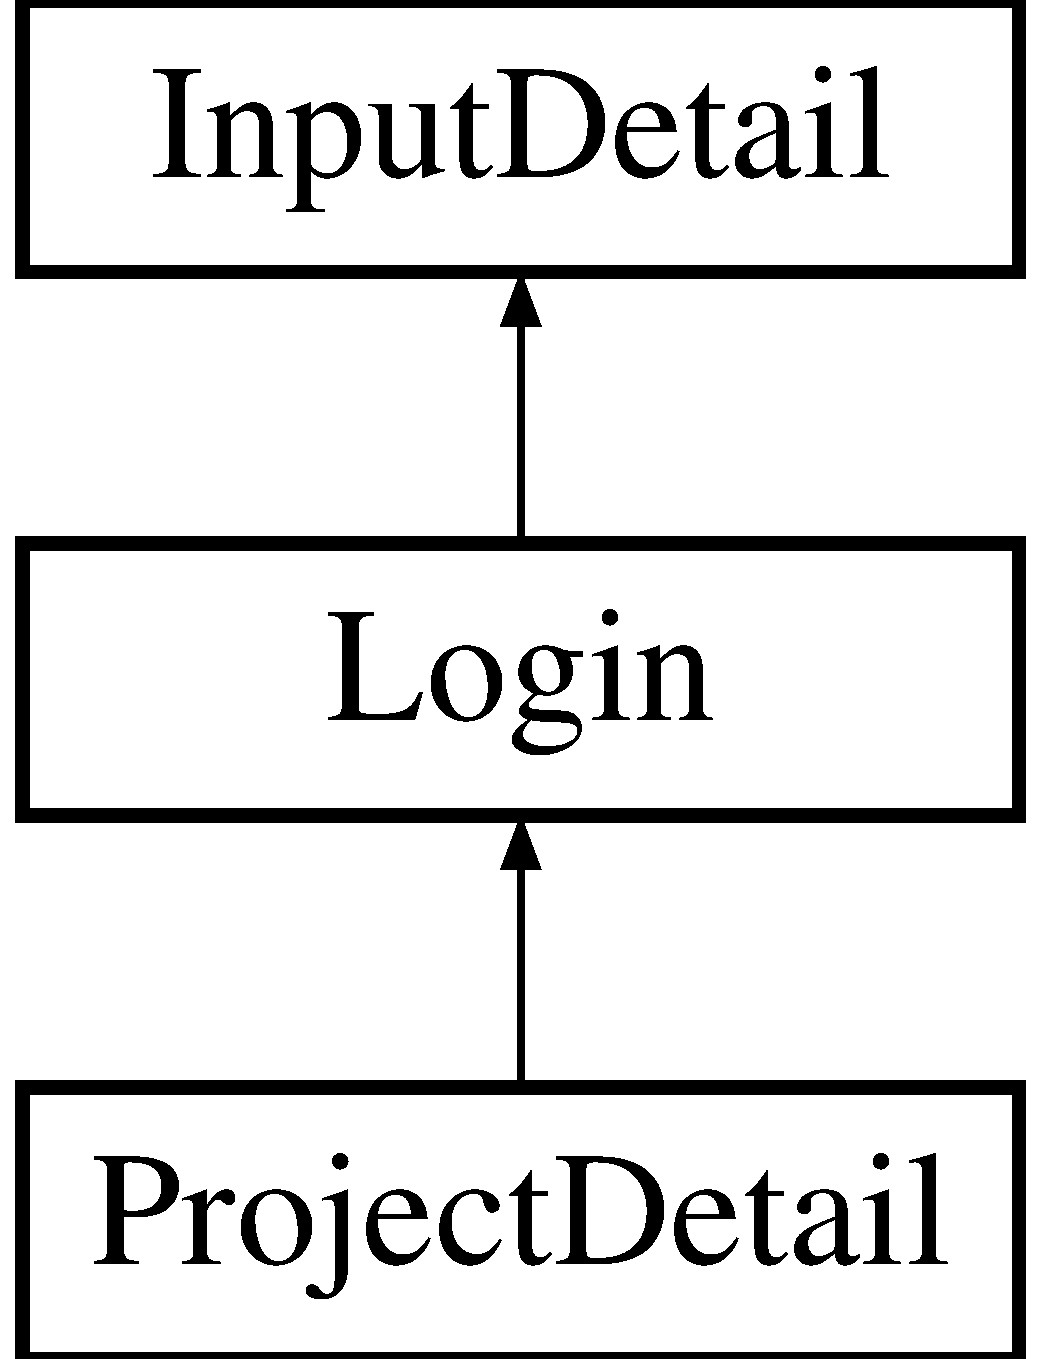
\includegraphics[height=3.000000cm]{dd/dfd/classLogin}
\end{center}
\end{figure}
\subsection*{\-Public \-Member \-Functions}
\begin{DoxyCompactItemize}
\item 
\hyperlink{classLogin_a4847f3e07e43b540d3339392346f87ff}{\-Login} ()
\begin{DoxyCompactList}\small\item\em \-Comstructor. \end{DoxyCompactList}\item 
void \hyperlink{classLogin_a2b2b36f506bcb5e7179b0b3afe164ace}{\-Login\-Page} (string \hyperlink{classInputDetail_a1abb16cd695678c3fa05e3c812823fee}{msg}=\char`\"{}\char`\"{}, string \hyperlink{classLogin_abea56d6d6403f1e627294f222dd77310}{email\-I\-D}=\char`\"{}abc@you.\-com\char`\"{}, string \hyperlink{classLogin_a39f7fd03b2b27c927c657ee73e7fcbbc}{password}=\char`\"{}\char`\"{})
\begin{DoxyCompactList}\small\item\em \-Function for creating login \-Page. \end{DoxyCompactList}\item 
void \hyperlink{classLogin_ab5bc65de431f277f15a3b423ad915808}{\-Read\-Login\-Detail} ()
\begin{DoxyCompactList}\small\item\em \-Reading login detail from text fields filled by user. \end{DoxyCompactList}\item 
void \hyperlink{classLogin_a3f4e5e4087c007e8e605849778881b39}{\-Registration\-Page} (string \hyperlink{classInputDetail_a1abb16cd695678c3fa05e3c812823fee}{msg}=\char`\"{}\char`\"{}, string \hyperlink{classLogin_abea56d6d6403f1e627294f222dd77310}{email\-I\-D}=\char`\"{}abc@you.\-com\char`\"{})
\begin{DoxyCompactList}\small\item\em \-For registering new user. \end{DoxyCompactList}\item 
void \hyperlink{classLogin_ae4f139afcb706f09b337befd123d5e18}{\-New\-User} ()
\begin{DoxyCompactList}\small\item\em \-Adding new user into database and if user already exists then move back to register page for unique email id. \end{DoxyCompactList}\item 
void \hyperlink{classLogin_ad127628ca09987d733477f90b828ad1e}{\-Select\-Login\-Detail} ()
\begin{DoxyCompactList}\small\item\em \-For reading email \-Id and password from \-User table in database. \end{DoxyCompactList}\item 
void \hyperlink{classLogin_a79ea5bbaeaa2ec6d21cd3195c522b863}{\-Confirm\-Page} (string \hyperlink{classInputDetail_a1abb16cd695678c3fa05e3c812823fee}{msg}=\char`\"{}\char`\"{}, string \hyperlink{classLogin_a39f7fd03b2b27c927c657ee73e7fcbbc}{password}=\char`\"{}\char`\"{}, string \hyperlink{classLogin_ade36f8943aafce470ef4b8353c79b2c6}{retype\-Password}=\char`\"{}\char`\"{})
\begin{DoxyCompactList}\small\item\em \-Page for validating email \-I\-D and setting user's password. \end{DoxyCompactList}\item 
void \hyperlink{classLogin_ac91737b2085d0b7e8943f49f2d08a0ff}{\-Add\-User} ()
\begin{DoxyCompactList}\small\item\em \-Add \-New user. \end{DoxyCompactList}\item 
void \hyperlink{classLogin_a4c5f4b15cce8b6bf325f35544f512fe2}{\-Reset\-Password\-Page} (string type=\char`\"{}1\char`\"{}, string \hyperlink{classInputDetail_a1abb16cd695678c3fa05e3c812823fee}{msg}=\char`\"{}\char`\"{}, string \hyperlink{classLogin_abea56d6d6403f1e627294f222dd77310}{email\-I\-D}=\char`\"{}abc@you.\-com\char`\"{})
\item 
void \hyperlink{classLogin_aa6978512971283a486347c3aa6ae0478}{\-Reset\-Password\-Form} (string type, string \hyperlink{classInputDetail_a1abb16cd695678c3fa05e3c812823fee}{msg}, string \hyperlink{classLogin_abea56d6d6403f1e627294f222dd77310}{email\-I\-D})
\item 
void \hyperlink{classLogin_a153d72df8d3333317e60219e8f6b8257}{\-Logout\-Page} ()
\begin{DoxyCompactList}\small\item\em \-Page for logging out. \end{DoxyCompactList}\item 
\hyperlink{classLogin_a659bc7233ec12c79b9fa523c1734fbbc}{$\sim$\-Login} ()
\end{DoxyCompactItemize}
\subsection*{\-Protected \-Attributes}
\begin{DoxyCompactItemize}
\item 
\-S\-T\-R\-I\-N\-G\-\_\-\-V\-E\-C \hyperlink{classLogin_abea56d6d6403f1e627294f222dd77310}{email\-I\-D}
\item 
\-S\-T\-R\-I\-N\-G\-\_\-\-V\-E\-C \hyperlink{classLogin_a39f7fd03b2b27c927c657ee73e7fcbbc}{password}
\item 
\-S\-T\-R\-I\-N\-G\-\_\-\-V\-E\-C \hyperlink{classLogin_ae22f0ed73e5248cd71a7b2167676376a}{reg\-Key}
\item 
string \hyperlink{classLogin_aa83b4706e0f0f0afc65f210ee8e4839a}{user\-Email\-I\-D}
\item 
string \hyperlink{classLogin_a9731be126468f535f161f045c95687c6}{user\-Password}
\item 
string \hyperlink{classLogin_ade36f8943aafce470ef4b8353c79b2c6}{retype\-Password}
\item 
string \hyperlink{classLogin_a624f15ecf989648b73a91743f67a6880}{current\-Time}
\item 
\hypertarget{classLogin_ab7769b44690490b43fc9046ad5958baf}{string {\bfseries key}}\label{dd/dfd/classLogin_ab7769b44690490b43fc9046ad5958baf}

\item 
\hypertarget{classLogin_a36ff1dd294aaaf884805325cee3b83d3}{\hyperlink{classSendMail}{\-Send\-Mail} {\bfseries send\-Mail}}\label{dd/dfd/classLogin_a36ff1dd294aaaf884805325cee3b83d3}

\end{DoxyCompactItemize}


\subsection{\-Detailed \-Description}
-\/-\/-\/-\/-\/-\/-\/-\/-\/-\/-\/-\/-\/-\/-\/-\/-\/-\/-\/-\/-\/-\/-\/-\/-\/-\/-\/-\/-\/-\/-\/-\/-\/-\/-\/-\/-\/-\/-\/-\/-\/-\/-\/-\/-\/-\/-\/-\/-\/-\/-\/-\/-\/-\/-\/-\/-\/-\/-\/-\/-\/-\/-\/-\/-\/-\/-\/ \-Include required header files -\/-\/-\/-\/-\/-\/-\/-\/-\/-\/-\/-\/-\/-\/-\/-\/-\/-\/-\/-\/-\/-\/-\/-\/-\/-\/-\/-\/-\/-\/-\/-\/-\/-\/-\/-\/-\/-\/-\/-\/-\/-\/-\/-\/-\/-\/-\/-\/-\/-\/-\/-\/-\/-\/-\/-\/-\/-\/-\/-\/-\/-\/-\/-\/-\/-\/ =================================================================== \-Class\-: \hyperlink{classLogin}{\-Login} \-Description\-: \hyperlink{classLogin}{\-Login} class for user login ===================================================================

\-Include \hyperlink{login_8h_source}{login.\-h} header file 

\-Definition at line 38 of file login.\-h.



\subsection{\-Constructor \& \-Destructor \-Documentation}
\hypertarget{classLogin_a4847f3e07e43b540d3339392346f87ff}{\index{\-Login@{\-Login}!\-Login@{\-Login}}
\index{\-Login@{\-Login}!Login@{\-Login}}
\subsubsection[{\-Login}]{\setlength{\rightskip}{0pt plus 5cm}{\bf \-Login\-::\-Login} (
\begin{DoxyParamCaption}
{}
\end{DoxyParamCaption}
)}}\label{dd/dfd/classLogin_a4847f3e07e43b540d3339392346f87ff}


\-Comstructor. 

\-Constructor 

\-Definition at line 32 of file login.\-cc.

\hypertarget{classLogin_a659bc7233ec12c79b9fa523c1734fbbc}{\index{\-Login@{\-Login}!$\sim$\-Login@{$\sim$\-Login}}
\index{$\sim$\-Login@{$\sim$\-Login}!Login@{\-Login}}
\subsubsection[{$\sim$\-Login}]{\setlength{\rightskip}{0pt plus 5cm}{\bf \-Login\-::$\sim$\-Login} (
\begin{DoxyParamCaption}
{}
\end{DoxyParamCaption}
)\hspace{0.3cm}{\ttfamily  \mbox{[}inline\mbox{]}}}}\label{dd/dfd/classLogin_a659bc7233ec12c79b9fa523c1734fbbc}
\-Destructor 

\-Definition at line 94 of file login.\-h.



\subsection{\-Member \-Function \-Documentation}
\hypertarget{classLogin_ac91737b2085d0b7e8943f49f2d08a0ff}{\index{\-Login@{\-Login}!\-Add\-User@{\-Add\-User}}
\index{\-Add\-User@{\-Add\-User}!Login@{\-Login}}
\subsubsection[{\-Add\-User}]{\setlength{\rightskip}{0pt plus 5cm}void {\bf \-Login\-::\-Add\-User} (
\begin{DoxyParamCaption}
{}
\end{DoxyParamCaption}
)}}\label{dd/dfd/classLogin_ac91737b2085d0b7e8943f49f2d08a0ff}


\-Add \-New user. 

\-Add new user 

\-Definition at line 273 of file login.\-cc.

\hypertarget{classLogin_a79ea5bbaeaa2ec6d21cd3195c522b863}{\index{\-Login@{\-Login}!\-Confirm\-Page@{\-Confirm\-Page}}
\index{\-Confirm\-Page@{\-Confirm\-Page}!Login@{\-Login}}
\subsubsection[{\-Confirm\-Page}]{\setlength{\rightskip}{0pt plus 5cm}void {\bf \-Login\-::\-Confirm\-Page} (
\begin{DoxyParamCaption}
\item[{string}]{msg = {\ttfamily \char`\"{}\char`\"{}}, }
\item[{string}]{password = {\ttfamily \char`\"{}\char`\"{}}, }
\item[{string}]{retype\-Password = {\ttfamily \char`\"{}\char`\"{}}}
\end{DoxyParamCaption}
)}}\label{dd/dfd/classLogin_a79ea5bbaeaa2ec6d21cd3195c522b863}


\-Page for validating email \-I\-D and setting user's password. 


\begin{DoxyParams}{\-Parameters}
{\em msg} & \-Shows error message \\
\hline
{\em password} & \-Password filled by user \\
\hline
{\em retype\-Password} & \-Password filled by user \\
\hline
\end{DoxyParams}


\-Definition at line 212 of file login.\-cc.

\hypertarget{classLogin_a2b2b36f506bcb5e7179b0b3afe164ace}{\index{\-Login@{\-Login}!\-Login\-Page@{\-Login\-Page}}
\index{\-Login\-Page@{\-Login\-Page}!Login@{\-Login}}
\subsubsection[{\-Login\-Page}]{\setlength{\rightskip}{0pt plus 5cm}void {\bf \-Login\-::\-Login\-Page} (
\begin{DoxyParamCaption}
\item[{string}]{msg = {\ttfamily \char`\"{}\char`\"{}}, }
\item[{string}]{email\-I\-D = {\ttfamily \char`\"{}abc@you.com\char`\"{}}, }
\item[{string}]{password = {\ttfamily \char`\"{}\char`\"{}}}
\end{DoxyParamCaption}
)}}\label{dd/dfd/classLogin_a2b2b36f506bcb5e7179b0b3afe164ace}


\-Function for creating login \-Page. 

\-Creating login page


\begin{DoxyParams}{\-Parameters}
{\em msg} & \-Show \-Message if email\-I\-D/ password incorrect \\
\hline
{\em emial\-I\-D} & user filled email id \\
\hline
{\em password} & uer password \\
\hline
\end{DoxyParams}


\-Definition at line 87 of file login.\-cc.

\hypertarget{classLogin_a153d72df8d3333317e60219e8f6b8257}{\index{\-Login@{\-Login}!\-Logout\-Page@{\-Logout\-Page}}
\index{\-Logout\-Page@{\-Logout\-Page}!Login@{\-Login}}
\subsubsection[{\-Logout\-Page}]{\setlength{\rightskip}{0pt plus 5cm}void {\bf \-Login\-::\-Logout\-Page} (
\begin{DoxyParamCaption}
{}
\end{DoxyParamCaption}
)}}\label{dd/dfd/classLogin_a153d72df8d3333317e60219e8f6b8257}


\-Page for logging out. 

\-Logout \-Page 

\-Definition at line 315 of file login.\-cc.

\hypertarget{classLogin_ae4f139afcb706f09b337befd123d5e18}{\index{\-Login@{\-Login}!\-New\-User@{\-New\-User}}
\index{\-New\-User@{\-New\-User}!Login@{\-Login}}
\subsubsection[{\-New\-User}]{\setlength{\rightskip}{0pt plus 5cm}void {\bf \-Login\-::\-New\-User} (
\begin{DoxyParamCaption}
{}
\end{DoxyParamCaption}
)}}\label{dd/dfd/classLogin_ae4f139afcb706f09b337befd123d5e18}


\-Adding new user into database and if user already exists then move back to register page for unique email id. 

\-Add new user in database 

\-Definition at line 172 of file login.\-cc.

\hypertarget{classLogin_ab5bc65de431f277f15a3b423ad915808}{\index{\-Login@{\-Login}!\-Read\-Login\-Detail@{\-Read\-Login\-Detail}}
\index{\-Read\-Login\-Detail@{\-Read\-Login\-Detail}!Login@{\-Login}}
\subsubsection[{\-Read\-Login\-Detail}]{\setlength{\rightskip}{0pt plus 5cm}void {\bf \-Login\-::\-Read\-Login\-Detail} (
\begin{DoxyParamCaption}
{}
\end{DoxyParamCaption}
)}}\label{dd/dfd/classLogin_ab5bc65de431f277f15a3b423ad915808}


\-Reading login detail from text fields filled by user. 

\-Read \hyperlink{classLogin}{\-Login} \-Detail


\begin{DoxyParams}{\-Parameters}
{\em } & \\
\hline
\end{DoxyParams}


\-Definition at line 71 of file login.\-cc.

\hypertarget{classLogin_a3f4e5e4087c007e8e605849778881b39}{\index{\-Login@{\-Login}!\-Registration\-Page@{\-Registration\-Page}}
\index{\-Registration\-Page@{\-Registration\-Page}!Login@{\-Login}}
\subsubsection[{\-Registration\-Page}]{\setlength{\rightskip}{0pt plus 5cm}void {\bf \-Login\-::\-Registration\-Page} (
\begin{DoxyParamCaption}
\item[{string}]{msg = {\ttfamily \char`\"{}\char`\"{}}, }
\item[{string}]{email\-I\-D = {\ttfamily \char`\"{}abc@you.com\char`\"{}}}
\end{DoxyParamCaption}
)}}\label{dd/dfd/classLogin_a3f4e5e4087c007e8e605849778881b39}


\-For registering new user. 

\-Register user page 

\-Definition at line 131 of file login.\-cc.

\hypertarget{classLogin_aa6978512971283a486347c3aa6ae0478}{\index{\-Login@{\-Login}!\-Reset\-Password\-Form@{\-Reset\-Password\-Form}}
\index{\-Reset\-Password\-Form@{\-Reset\-Password\-Form}!Login@{\-Login}}
\subsubsection[{\-Reset\-Password\-Form}]{\setlength{\rightskip}{0pt plus 5cm}void {\bf \-Login\-::\-Reset\-Password\-Form} (
\begin{DoxyParamCaption}
\item[{string}]{type, }
\item[{string}]{msg, }
\item[{string}]{email\-I\-D}
\end{DoxyParamCaption}
)}}\label{dd/dfd/classLogin_aa6978512971283a486347c3aa6ae0478}
\-Reset \-Password \-Forms 

\-Definition at line 347 of file login.\-cc.

\hypertarget{classLogin_a4c5f4b15cce8b6bf325f35544f512fe2}{\index{\-Login@{\-Login}!\-Reset\-Password\-Page@{\-Reset\-Password\-Page}}
\index{\-Reset\-Password\-Page@{\-Reset\-Password\-Page}!Login@{\-Login}}
\subsubsection[{\-Reset\-Password\-Page}]{\setlength{\rightskip}{0pt plus 5cm}void {\bf \-Login\-::\-Reset\-Password\-Page} (
\begin{DoxyParamCaption}
\item[{string}]{type = {\ttfamily \char`\"{}1\char`\"{}}, }
\item[{string}]{msg = {\ttfamily \char`\"{}\char`\"{}}, }
\item[{string}]{email\-I\-D = {\ttfamily \char`\"{}abc@you.com\char`\"{}}}
\end{DoxyParamCaption}
)}}\label{dd/dfd/classLogin_a4c5f4b15cce8b6bf325f35544f512fe2}
\-Reset password of existing user 

\-Definition at line 325 of file login.\-cc.

\hypertarget{classLogin_ad127628ca09987d733477f90b828ad1e}{\index{\-Login@{\-Login}!\-Select\-Login\-Detail@{\-Select\-Login\-Detail}}
\index{\-Select\-Login\-Detail@{\-Select\-Login\-Detail}!Login@{\-Login}}
\subsubsection[{\-Select\-Login\-Detail}]{\setlength{\rightskip}{0pt plus 5cm}void {\bf \-Login\-::\-Select\-Login\-Detail} (
\begin{DoxyParamCaption}
{}
\end{DoxyParamCaption}
)}}\label{dd/dfd/classLogin_ad127628ca09987d733477f90b828ad1e}


\-For reading email \-Id and password from \-User table in database. 

\-For selecting emial and password fron user table 

\-Definition at line 44 of file login.\-cc.



\subsection{\-Member \-Data \-Documentation}
\hypertarget{classLogin_a624f15ecf989648b73a91743f67a6880}{\index{\-Login@{\-Login}!current\-Time@{current\-Time}}
\index{current\-Time@{current\-Time}!Login@{\-Login}}
\subsubsection[{current\-Time}]{\setlength{\rightskip}{0pt plus 5cm}string {\bf \-Login\-::current\-Time}\hspace{0.3cm}{\ttfamily  \mbox{[}protected\mbox{]}}}}\label{dd/dfd/classLogin_a624f15ecf989648b73a91743f67a6880}
\-Currennt \-Time 

\-Definition at line 51 of file login.\-h.

\hypertarget{classLogin_abea56d6d6403f1e627294f222dd77310}{\index{\-Login@{\-Login}!email\-I\-D@{email\-I\-D}}
\index{email\-I\-D@{email\-I\-D}!Login@{\-Login}}
\subsubsection[{email\-I\-D}]{\setlength{\rightskip}{0pt plus 5cm}\-S\-T\-R\-I\-N\-G\-\_\-\-V\-E\-C {\bf \-Login\-::email\-I\-D}\hspace{0.3cm}{\ttfamily  \mbox{[}protected\mbox{]}}}}\label{dd/dfd/classLogin_abea56d6d6403f1e627294f222dd77310}
\-For storting email and password of users \-Email \-I\-D as vector 

\-Reimplemented from \hyperlink{classInputDetail_ad3f1db4fddbe0d4efbf1d5bc74d52257}{\-Input\-Detail}.



\-Definition at line 43 of file login.\-h.

\hypertarget{classLogin_a39f7fd03b2b27c927c657ee73e7fcbbc}{\index{\-Login@{\-Login}!password@{password}}
\index{password@{password}!Login@{\-Login}}
\subsubsection[{password}]{\setlength{\rightskip}{0pt plus 5cm}\-S\-T\-R\-I\-N\-G\-\_\-\-V\-E\-C {\bf \-Login\-::password}\hspace{0.3cm}{\ttfamily  \mbox{[}protected\mbox{]}}}}\label{dd/dfd/classLogin_a39f7fd03b2b27c927c657ee73e7fcbbc}
password as vector variable 

\-Definition at line 43 of file login.\-h.

\hypertarget{classLogin_ae22f0ed73e5248cd71a7b2167676376a}{\index{\-Login@{\-Login}!reg\-Key@{reg\-Key}}
\index{reg\-Key@{reg\-Key}!Login@{\-Login}}
\subsubsection[{reg\-Key}]{\setlength{\rightskip}{0pt plus 5cm}\-S\-T\-R\-I\-N\-G\-\_\-\-V\-E\-C {\bf \-Login\-::reg\-Key}\hspace{0.3cm}{\ttfamily  \mbox{[}protected\mbox{]}}}}\label{dd/dfd/classLogin_ae22f0ed73e5248cd71a7b2167676376a}
\-Registration key 

\-Definition at line 43 of file login.\-h.

\hypertarget{classLogin_ade36f8943aafce470ef4b8353c79b2c6}{\index{\-Login@{\-Login}!retype\-Password@{retype\-Password}}
\index{retype\-Password@{retype\-Password}!Login@{\-Login}}
\subsubsection[{retype\-Password}]{\setlength{\rightskip}{0pt plus 5cm}string {\bf \-Login\-::retype\-Password}\hspace{0.3cm}{\ttfamily  \mbox{[}protected\mbox{]}}}}\label{dd/dfd/classLogin_ade36f8943aafce470ef4b8353c79b2c6}
\-For reading password 

\-Definition at line 47 of file login.\-h.

\hypertarget{classLogin_aa83b4706e0f0f0afc65f210ee8e4839a}{\index{\-Login@{\-Login}!user\-Email\-I\-D@{user\-Email\-I\-D}}
\index{user\-Email\-I\-D@{user\-Email\-I\-D}!Login@{\-Login}}
\subsubsection[{user\-Email\-I\-D}]{\setlength{\rightskip}{0pt plus 5cm}string {\bf \-Login\-::user\-Email\-I\-D}\hspace{0.3cm}{\ttfamily  \mbox{[}protected\mbox{]}}}}\label{dd/dfd/classLogin_aa83b4706e0f0f0afc65f210ee8e4839a}
\-For reading email\-I\-D in text field 

\-Definition at line 47 of file login.\-h.

\hypertarget{classLogin_a9731be126468f535f161f045c95687c6}{\index{\-Login@{\-Login}!user\-Password@{user\-Password}}
\index{user\-Password@{user\-Password}!Login@{\-Login}}
\subsubsection[{user\-Password}]{\setlength{\rightskip}{0pt plus 5cm}string {\bf \-Login\-::user\-Password}\hspace{0.3cm}{\ttfamily  \mbox{[}protected\mbox{]}}}}\label{dd/dfd/classLogin_a9731be126468f535f161f045c95687c6}
\-For reading password in text field 

\-Definition at line 47 of file login.\-h.



\-The documentation for this class was generated from the following files\-:\begin{DoxyCompactItemize}
\item 
frontend/src/header/login.\-h\item 
frontend/src/login.\-cc\end{DoxyCompactItemize}

\hypertarget{classMD5}{\section{M\-D5 Class Reference}
\label{classMD5}\index{M\-D5@{M\-D5}}
}
\subsection*{Public Types}
\begin{DoxyCompactItemize}
\item 
\hypertarget{classMD5_aa836972700679dbcff6ae8337f6db464}{typedef unsigned int {\bfseries size\-\_\-type}}\label{classMD5_aa836972700679dbcff6ae8337f6db464}

\end{DoxyCompactItemize}
\subsection*{Public Member Functions}
\begin{DoxyCompactItemize}
\item 
\hypertarget{classMD5_a155356ffd713345e69e6dcbd9f8da6ce}{{\bfseries M\-D5} (const std\-::string \&text)}\label{classMD5_a155356ffd713345e69e6dcbd9f8da6ce}

\item 
\hypertarget{classMD5_ac5ddf6cd8f940422396d321ea90ed045}{void {\bfseries update} (const unsigned char $\ast$buf, size\-\_\-type length)}\label{classMD5_ac5ddf6cd8f940422396d321ea90ed045}

\item 
\hypertarget{classMD5_ac5ccba375539b993958fb235f8ac849c}{void {\bfseries update} (const char $\ast$buf, size\-\_\-type length)}\label{classMD5_ac5ccba375539b993958fb235f8ac849c}

\item 
\hypertarget{classMD5_a10f607494a3f2e3e515fc4b99d1a06cc}{\hyperlink{classMD5}{M\-D5} \& {\bfseries finalize} ()}\label{classMD5_a10f607494a3f2e3e515fc4b99d1a06cc}

\item 
\hypertarget{classMD5_ad36c65acf87e397bf717bc3defbc0c7a}{std\-::string {\bfseries hexdigest} () const }\label{classMD5_ad36c65acf87e397bf717bc3defbc0c7a}

\end{DoxyCompactItemize}
\subsection*{Friends}
\begin{DoxyCompactItemize}
\item 
\hypertarget{classMD5_a0739666fd0f3a7117546f6c50e0783b2}{std\-::ostream \& {\bfseries operator$<$$<$} (std\-::ostream \&, \hyperlink{classMD5}{M\-D5} md5)}\label{classMD5_a0739666fd0f3a7117546f6c50e0783b2}

\end{DoxyCompactItemize}


\subsection{Detailed Description}


Definition at line 69 of file md5.\-h.



The documentation for this class was generated from the following files\-:\begin{DoxyCompactItemize}
\item 
src/header/md5.\-h\item 
src/md5.\-cc\end{DoxyCompactItemize}

\hypertarget{classPageLayout}{\section{Page\-Layout Class Reference}
\label{classPageLayout}\index{Page\-Layout@{Page\-Layout}}
}


{\ttfamily \#include $<$pagelayout.\-h$>$}

Inheritance diagram for Page\-Layout\-:\begin{figure}[H]
\begin{center}
\leavevmode
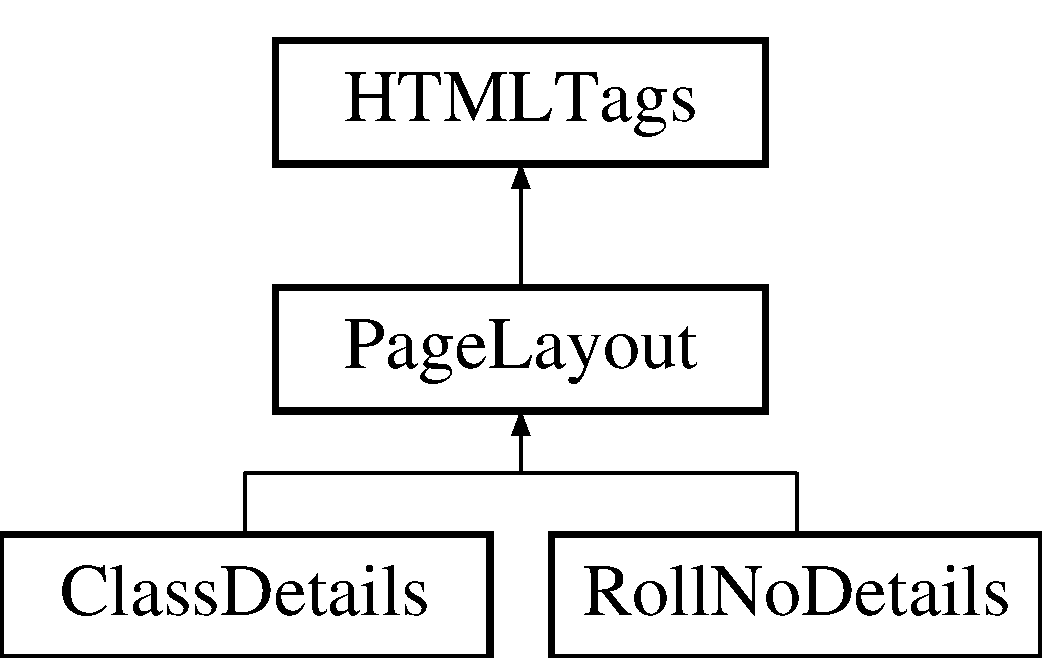
\includegraphics[height=5.000000cm]{classPageLayout}
\end{center}
\end{figure}
\subsection*{Public Member Functions}
\begin{DoxyCompactItemize}
\item 
\hyperlink{classPageLayout_ab3f470f006f9820610d9aaebe5b8427b}{Page\-Layout} ()
\item 
void \hyperlink{classPageLayout_a7726061f0653245f644a05807fa92472}{Header} ()
\item 
void \hyperlink{classPageLayout_a68aa868a8868b12964f161838b5f814c}{Footer} ()
\item 
void \hyperlink{classPageLayout_a49af1dca286bbee9432192a7b3c00332}{Menu} ()
\item 
void \hyperlink{classPageLayout_ae60235c6af48e3ebbc6343d02456da0c}{Logo} (string logo\-Name)
\item 
void \hyperlink{classPageLayout_ae50907d56f0ba7a85f7ccfdeafa45bcc}{Head} (string title\-Name)
\item 
void \hyperlink{classPageLayout_a449b4dde24cf3dc10299dc3c7bfc0e9c}{Set\-Cookies} (string email\-I\-D, string \hyperlink{classPageLayout_ab796c4a12a3f9c089881085e508e2a1c}{session\-I\-D})
\item 
void \hyperlink{classPageLayout_a9884173383d3e9b91e5b4ba6a619caa9}{Context\-Type} ()
\item 
void \hyperlink{classPageLayout_abe2cfa43480c1b48125b3d618cab7831}{Logout\-Link} ()
\item 
void \hyperlink{classPageStructureMaker_aaf78d67380c400cc0057c6519276f721}{Set\-H\-T\-M\-L\-Variables} ()
\item 
void \hyperlink{classPageStructureMaker_ad25d6abc983253567e2370882fc1b407}{H\-T\-M\-L\-Start} ()
\item 
void \hyperlink{classPageStructureMaker_a63b877af1c2c8de8332e3f7eb4c2c2b0}{H\-T\-M\-L\-End} ()
\item 
void \hyperlink{classPageStructureMaker_a14312134cb108f91f2e6d9cbd6916e97}{Head\-Start} ()
\item 
void \hyperlink{classPageStructureMaker_ad64115d592b0989b422a93f85278186e}{Head\-End} ()
\item 
void \hyperlink{classPageStructureMaker_a81e902ddc0c0287df1ba0f614a3774d6}{Title} (string page\-Title)
\item 
void \hyperlink{classPageStructureMaker_aacdb11817f8ab246bc59c552e04e862d}{C\-S\-S} (string href)
\item 
void \hyperlink{classPageStructureMaker_ac221d1169f4dbcef6adb00938919193d}{Javascript} (string src)
\item 
void \hyperlink{classPageStructureMaker_ab7a645675166f34fac99f1ed8feb7c27}{Body\-Start} ()
\item 
void \hyperlink{classPageStructureMaker_ac91e234e2d54dedd9d7e556fabf21d2b}{Body\-End} ()
\item 
void \hyperlink{classPageStructureMaker_a927f92889555dd316c129f706be86a5c}{Div\-Start} (string id, string class\-Name)
\item 
void \hyperlink{classPageStructureMaker_a2913e76bf188ed777dcd33003ef6207d}{Div\-End} ()
\item 
void \hyperlink{classPageStructureMaker_a3f25d5b844a2251883acb80d8fabb77d}{Form\-Start} (string name, string action, string method)
\item 
void \hyperlink{classPageStructureMaker_a65d97f23bb543f3db5201b2009f7f65a}{Form\-End} ()
\item 
void \hyperlink{classPageStructureMaker_a04e68e69005f3933e0f496c3db474daf}{Table\-Start} (string id, string class\-Name)
\item 
void \hyperlink{classPageStructureMaker_a7f8fefbe7a825c1b7761fc8a0f1bb8e4}{Table\-End} ()
\item 
void \hyperlink{classPageStructureMaker_ac24ce26202757aaa30402155daf8a3d0}{List\-Start} (string list\-Type)
\item 
void \hyperlink{classPageStructureMaker_a8578b1555ad2fc92a9efc7dbf7d1fe87}{List\-End} (string list\-Type)
\item 
void \hyperlink{classPageStructureMaker_adf4116e526026edc3c8a3bcf96a7e929}{List\-Item} (string list\-Item)
\item 
void \hyperlink{classPageStructureMaker_a8c0fae5b599182863066de56ae0cea42}{Anchor} (string href, string target)
\item 
void \hyperlink{classPageStructureMaker_a3547027801e298307527f1e934787b13}{Input\-Field} (string type, string name, int name\-No, string value)
\item 
void \hyperlink{classPageStructureMaker_a928ea6f84a8f7833c128034068a4b9a7}{Input\-Field} (string type, string name, string value)
\item 
void \hyperlink{classPageStructureMaker_ae8684bb66ca463e2f92e09c96137f9e3}{Select\-Field\-Start} (string name)
\item 
void \hyperlink{classPageStructureMaker_a81eb3cdbc840a4c8165cef87330ade09}{Select\-Field\-End} ()
\item 
void \hyperlink{classPageStructureMaker_a77856078e74dab25329132ea07466f92}{Select\-Option\-Start} (string value, string selected)
\item 
void \hyperlink{classPageStructureMaker_a7682f479f7f1012d426ec9f9535def60}{Select\-Option\-End} ()
\item 
void \hyperlink{classPageStructureMaker_a419feca1cfdb50e1be757eb1c2707a73}{Button} (string id, string type, string class\-Name, string value)
\end{DoxyCompactItemize}
\subsection*{Protected Attributes}
\begin{DoxyCompactItemize}
\item 
\hypertarget{classPageLayout_a8a3c1ddc422df2556fbc95d0cd575a05}{string {\bfseries project\-Name}}\label{classPageLayout_a8a3c1ddc422df2556fbc95d0cd575a05}

\item 
\hypertarget{classPageLayout_a9abec89a54a6f0dac84114919d2ad117}{ifstream {\bfseries in\-File}}\label{classPageLayout_a9abec89a54a6f0dac84114919d2ad117}

\item 
\hypertarget{classPageLayout_ad52913274f786e82e1e09f5df4bf5347}{ofstream {\bfseries out\-File}}\label{classPageLayout_ad52913274f786e82e1e09f5df4bf5347}

\item 
string \hyperlink{classPageLayout_ab796c4a12a3f9c089881085e508e2a1c}{session\-I\-D}
\item 
string \hyperlink{classPageStructureMaker_af41d4e21b808f5f8dc2c727f775b6fb2}{start\-H1}
\item 
\hypertarget{classPageStructureMaker_a3786a6f477632e4a60205a988d6b599d}{string {\bfseries end\-H1}}\label{classPageStructureMaker_a3786a6f477632e4a60205a988d6b599d}

\item 
\hypertarget{classPageStructureMaker_adb966c147c6328c8e48281c882de776d}{string {\bfseries start\-H3}}\label{classPageStructureMaker_adb966c147c6328c8e48281c882de776d}

\item 
\hypertarget{classPageStructureMaker_a22e6bf3eb787284b745d694613c1d9da}{string {\bfseries end\-H3}}\label{classPageStructureMaker_a22e6bf3eb787284b745d694613c1d9da}

\item 
\hypertarget{classPageStructureMaker_a7e458e675a3adf987a153e08f3795941}{string {\bfseries start\-T\-D}}\label{classPageStructureMaker_a7e458e675a3adf987a153e08f3795941}

\item 
\hypertarget{classPageStructureMaker_ad27f03939a04048a03be0f1bb8edd38a}{string {\bfseries end\-T\-D}}\label{classPageStructureMaker_ad27f03939a04048a03be0f1bb8edd38a}

\item 
\hypertarget{classPageStructureMaker_a4fe234b016efcb9eaa757879b8858190}{string {\bfseries start\-T\-H}}\label{classPageStructureMaker_a4fe234b016efcb9eaa757879b8858190}

\item 
\hypertarget{classPageStructureMaker_aa244b4ef71850dc76fcfb5157bcaf8fc}{string {\bfseries end\-T\-H}}\label{classPageStructureMaker_aa244b4ef71850dc76fcfb5157bcaf8fc}

\item 
\hypertarget{classPageStructureMaker_aa59b4949d26fab5a72710fa9fc3e8ea9}{string {\bfseries start\-T\-R}}\label{classPageStructureMaker_aa59b4949d26fab5a72710fa9fc3e8ea9}

\item 
\hypertarget{classPageStructureMaker_afee49ebdcbc0971142fcf7eae8baa306}{string {\bfseries end\-T\-R}}\label{classPageStructureMaker_afee49ebdcbc0971142fcf7eae8baa306}

\item 
\hypertarget{classPageStructureMaker_aa0f624b485f07f6e19151b1df3dc59a3}{string {\bfseries start\-B}}\label{classPageStructureMaker_aa0f624b485f07f6e19151b1df3dc59a3}

\item 
\hypertarget{classPageStructureMaker_ad46c3195310a1f0226e21d2eb5befb00}{string {\bfseries end\-B}}\label{classPageStructureMaker_ad46c3195310a1f0226e21d2eb5befb00}

\item 
\hypertarget{classPageStructureMaker_a63911cb925ccdc6c879905a677ed8881}{string {\bfseries brk}}\label{classPageStructureMaker_a63911cb925ccdc6c879905a677ed8881}

\end{DoxyCompactItemize}


\subsection{Detailed Description}
-\/-\/-\/-\/-\/-\/-\/-\/-\/-\/-\/-\/-\/-\/-\/-\/-\/-\/-\/-\/-\/-\/-\/-\/-\/-\/-\/-\/-\/-\/-\/-\/-\/-\/-\/-\/-\/-\/-\/-\/-\/-\/-\/-\/-\/-\/-\/-\/-\/-\/-\/-\/-\/-\/-\/-\/-\/-\/-\/-\/-\/-\/-\/-\/-\/-\/-\/ Include required header files ------------------------------------------------------------------ =================================================================== Class\-: \hyperlink{classPageLayout}{Page\-Layout} \-: public \hyperlink{classPageStructureMaker}{Page\-Structure\-Maker} Description\-: For adding header and footer to page =================================================================== 

Definition at line 33 of file pagelayout.\-h.



\subsection{Constructor \& Destructor Documentation}
\hypertarget{classPageLayout_ab3f470f006f9820610d9aaebe5b8427b}{\index{Page\-Layout@{Page\-Layout}!Page\-Layout@{Page\-Layout}}
\index{Page\-Layout@{Page\-Layout}!PageLayout@{Page\-Layout}}
\subsubsection[{Page\-Layout}]{\setlength{\rightskip}{0pt plus 5cm}Page\-Layout\-::\-Page\-Layout (
\begin{DoxyParamCaption}
{}
\end{DoxyParamCaption}
)}}\label{classPageLayout_ab3f470f006f9820610d9aaebe5b8427b}
Constructor

-\/-\/-\/-\/-\/-\/-\/-\/-\/-\/-\/-\/-\/-\/-\/-\/-\/-\/-\/-\/-\/-\/-\/-\/-\/-\/-\/-\/-\/-\/-\/-\/-\/-\/-\/-\/-\/-\/-\/-\/-\/-\/-\/-\/-\/-\/-\/-\/-\/-\/-\/-\/-\/-\/-\/-\/-\/-\/-\/-\/-\/-\/-\/-\/-\/-\/-\/ Include local header file ------------------------------------------------------------------ -\/-\/-\/-\/-\/-\/-\/-\/-\/-\/-\/-\/-\/-\/-\/-\/-\/-\/-\/-\/-\/-\/-\/-\/-\/-\/-\/-\/-\/-\/-\/-\/-\/-\/-\/-\/-\/-\/-\/-\/-\/-\/-\/-\/-\/-\/-\/-\/-\/-\/-\/-\/-\/-\/-\/-\/-\/-\/-\/-\/-\/-\/-\/-\/-\/-\/-\/ Function Definitions of \hyperlink{classPageLayout}{Page\-Layout} Class ------------------------------------------------------------------ -\/-\/-\/-\/-\/-\/-\/-\/-\/-\/-\/-\/-\/-\/-\/-\/-\/-\/-\/-\/-\/-\/-\/-\/-\/-\/-\/-\/-\/-\/-\/-\/-\/-\/-\/-\/-\/-\/-\/-\/-\/-\/-\/-\/-\/-\/-\/-\/-\/-\/-\/-\/-\/-\/-\/-\/-\/-\/-\/-\/-\/-\/-\/-\/-\/-\/-\/-\/ Class\-: \hyperlink{classPageLayout}{Page\-Layout} Method\-: \hyperlink{classPageLayout}{Page\-Layout} \-:\-: \hyperlink{classPageLayout_ab3f470f006f9820610d9aaebe5b8427b}{Page\-Layout()} Description\-: Constructor -\/-\/-\/-\/-\/-\/-\/-\/-\/-\/-\/-\/-\/-\/-\/-\/-\/-\/-\/-\/-\/-\/-\/-\/-\/-\/-\/-\/-\/-\/-\/-\/-\/-\/-\/-\/-\/-\/-\/-\/-\/-\/-\/-\/-\/-\/-\/-\/-\/-\/-\/-\/-\/-\/-\/-\/-\/-\/-\/-\/-\/-\/-\/-\/-\/-\/-\/-\/ 

Definition at line 38 of file pagelayout.\-cc.



\subsection{Member Function Documentation}
\hypertarget{classPageStructureMaker_a8c0fae5b599182863066de56ae0cea42}{\index{Page\-Layout@{Page\-Layout}!Anchor@{Anchor}}
\index{Anchor@{Anchor}!PageLayout@{Page\-Layout}}
\subsubsection[{Anchor}]{\setlength{\rightskip}{0pt plus 5cm}void Page\-Structure\-Maker\-::\-Anchor (
\begin{DoxyParamCaption}
\item[{string}]{href, }
\item[{string}]{target}
\end{DoxyParamCaption}
)\hspace{0.3cm}{\ttfamily [inherited]}}}\label{classPageStructureMaker_a8c0fae5b599182863066de56ae0cea42}
Anchor Tag

--------------------------------------------------------------------\par
 Class\-: \hyperlink{classPageStructureMaker}{Page\-Structure\-Maker} \par
 Method\-: \hyperlink{classPageStructureMaker}{Page\-Structure\-Maker} \-:\-: Anchor(string href) \par
 Description\-: Anchor Tag \par
 -\/-\/-\/-\/-\/-\/-\/-\/-\/-\/-\/-\/-\/-\/-\/-\/-\/-\/-\/-\/-\/-\/-\/-\/-\/-\/-\/-\/-\/-\/-\/-\/-\/-\/-\/-\/-\/-\/-\/-\/-\/-\/-\/-\/-\/-\/-\/-\/-\/-\/-\/-\/-\/-\/-\/-\/-\/-\/-\/-\/-\/-\/-\/-\/-\/-\/-\/-\/ 

Definition at line 318 of file pagestructure.\-cc.

\hypertarget{classPageStructureMaker_ac91e234e2d54dedd9d7e556fabf21d2b}{\index{Page\-Layout@{Page\-Layout}!Body\-End@{Body\-End}}
\index{Body\-End@{Body\-End}!PageLayout@{Page\-Layout}}
\subsubsection[{Body\-End}]{\setlength{\rightskip}{0pt plus 5cm}void Page\-Structure\-Maker\-::\-Body\-End (
\begin{DoxyParamCaption}
{}
\end{DoxyParamCaption}
)\hspace{0.3cm}{\ttfamily [inherited]}}}\label{classPageStructureMaker_ac91e234e2d54dedd9d7e556fabf21d2b}
Display $<$/\-B\-O\-D\-Y$>$

-\/-\/-\/-\/-\/-\/-\/-\/-\/-\/-\/-\/-\/-\/-\/-\/-\/-\/-\/-\/-\/-\/-\/-\/-\/-\/-\/-\/-\/-\/-\/-\/-\/-\/-\/-\/-\/-\/-\/-\/-\/-\/-\/-\/-\/-\/-\/-\/-\/-\/-\/-\/-\/-\/-\/-\/-\/-\/-\/-\/-\/-\/-\/-\/-\/-\/-\/-\/ Class\-: \hyperlink{classPageStructureMaker}{Page\-Structure\-Maker} Method\-: \hyperlink{classPageStructureMaker}{Page\-Structure\-Maker} \-:\-: \hyperlink{classPageStructureMaker_ac91e234e2d54dedd9d7e556fabf21d2b}{Body\-End()} Description\-: Display $<$/\-B\-O\-D\-Y$>$ -\/-\/-\/-\/-\/-\/-\/-\/-\/-\/-\/-\/-\/-\/-\/-\/-\/-\/-\/-\/-\/-\/-\/-\/-\/-\/-\/-\/-\/-\/-\/-\/-\/-\/-\/-\/-\/-\/-\/-\/-\/-\/-\/-\/-\/-\/-\/-\/-\/-\/-\/-\/-\/-\/-\/-\/-\/-\/-\/-\/-\/-\/-\/-\/-\/-\/-\/-\/ 

Definition at line 180 of file pagestructure.\-cc.

\hypertarget{classPageStructureMaker_ab7a645675166f34fac99f1ed8feb7c27}{\index{Page\-Layout@{Page\-Layout}!Body\-Start@{Body\-Start}}
\index{Body\-Start@{Body\-Start}!PageLayout@{Page\-Layout}}
\subsubsection[{Body\-Start}]{\setlength{\rightskip}{0pt plus 5cm}void Page\-Structure\-Maker\-::\-Body\-Start (
\begin{DoxyParamCaption}
{}
\end{DoxyParamCaption}
)\hspace{0.3cm}{\ttfamily [inherited]}}}\label{classPageStructureMaker_ab7a645675166f34fac99f1ed8feb7c27}
Display $<$\-B\-O\-D\-Y$>$

-\/-\/-\/-\/-\/-\/-\/-\/-\/-\/-\/-\/-\/-\/-\/-\/-\/-\/-\/-\/-\/-\/-\/-\/-\/-\/-\/-\/-\/-\/-\/-\/-\/-\/-\/-\/-\/-\/-\/-\/-\/-\/-\/-\/-\/-\/-\/-\/-\/-\/-\/-\/-\/-\/-\/-\/-\/-\/-\/-\/-\/-\/-\/-\/-\/-\/-\/-\/ Class\-: \hyperlink{classPageStructureMaker}{Page\-Structure\-Maker} Method\-: \hyperlink{classPageStructureMaker}{Page\-Structure\-Maker} \-:\-: \hyperlink{classPageStructureMaker_ab7a645675166f34fac99f1ed8feb7c27}{Body\-Start()} Description\-: Display $<$B\-O\-D\-Y$>$ -\/-\/-\/-\/-\/-\/-\/-\/-\/-\/-\/-\/-\/-\/-\/-\/-\/-\/-\/-\/-\/-\/-\/-\/-\/-\/-\/-\/-\/-\/-\/-\/-\/-\/-\/-\/-\/-\/-\/-\/-\/-\/-\/-\/-\/-\/-\/-\/-\/-\/-\/-\/-\/-\/-\/-\/-\/-\/-\/-\/-\/-\/-\/-\/-\/-\/-\/-\/ 

Definition at line 166 of file pagestructure.\-cc.

\hypertarget{classPageStructureMaker_a419feca1cfdb50e1be757eb1c2707a73}{\index{Page\-Layout@{Page\-Layout}!Button@{Button}}
\index{Button@{Button}!PageLayout@{Page\-Layout}}
\subsubsection[{Button}]{\setlength{\rightskip}{0pt plus 5cm}void Page\-Structure\-Maker\-::\-Button (
\begin{DoxyParamCaption}
\item[{string}]{id, }
\item[{string}]{type, }
\item[{string}]{class\-Name, }
\item[{string}]{value}
\end{DoxyParamCaption}
)\hspace{0.3cm}{\ttfamily [inherited]}}}\label{classPageStructureMaker_a419feca1cfdb50e1be757eb1c2707a73}
Button

-\/-\/-\/-\/-\/-\/-\/-\/-\/-\/-\/-\/-\/-\/-\/-\/-\/-\/-\/-\/-\/-\/-\/-\/-\/-\/-\/-\/-\/-\/-\/-\/-\/-\/-\/-\/-\/-\/-\/-\/-\/-\/-\/-\/-\/-\/-\/-\/-\/-\/-\/-\/-\/-\/-\/-\/-\/-\/-\/-\/-\/-\/-\/-\/-\/-\/-\/-\/ Class\-: \hyperlink{classPageStructureMaker}{Page\-Structure\-Maker} Method\-: \hyperlink{classPageStructureMaker}{Page\-Structure\-Maker} \-:\-: Button(string id, string type, string class\-Name, string value) Description\-: Create button(next, submit, etc) -\/-\/-\/-\/-\/-\/-\/-\/-\/-\/-\/-\/-\/-\/-\/-\/-\/-\/-\/-\/-\/-\/-\/-\/-\/-\/-\/-\/-\/-\/-\/-\/-\/-\/-\/-\/-\/-\/-\/-\/-\/-\/-\/-\/-\/-\/-\/-\/-\/-\/-\/-\/-\/-\/-\/-\/-\/-\/-\/-\/-\/-\/-\/-\/-\/-\/-\/-\/ 

Definition at line 436 of file pagestructure.\-cc.

\hypertarget{classPageLayout_a9884173383d3e9b91e5b4ba6a619caa9}{\index{Page\-Layout@{Page\-Layout}!Context\-Type@{Context\-Type}}
\index{Context\-Type@{Context\-Type}!PageLayout@{Page\-Layout}}
\subsubsection[{Context\-Type}]{\setlength{\rightskip}{0pt plus 5cm}void Page\-Layout\-::\-Context\-Type (
\begin{DoxyParamCaption}
{}
\end{DoxyParamCaption}
)}}\label{classPageLayout_a9884173383d3e9b91e5b4ba6a619caa9}
Context-\/\-Type header

--------------------------------------------------------------------\par
 Class\-: \hyperlink{classPageLayout}{Page\-Layout} \par
 Method\-: \hyperlink{classPageLayout}{Page\-Layout} \-:\-: Context\-Type \par
 Description\-: Setting content-\/type header \par
 -\/-\/-\/-\/-\/-\/-\/-\/-\/-\/-\/-\/-\/-\/-\/-\/-\/-\/-\/-\/-\/-\/-\/-\/-\/-\/-\/-\/-\/-\/-\/-\/-\/-\/-\/-\/-\/-\/-\/-\/-\/-\/-\/-\/-\/-\/-\/-\/-\/-\/-\/-\/-\/-\/-\/-\/-\/-\/-\/-\/-\/-\/-\/-\/-\/-\/-\/-\/ 

Definition at line 162 of file pagelayout.\-cc.

\hypertarget{classPageStructureMaker_aacdb11817f8ab246bc59c552e04e862d}{\index{Page\-Layout@{Page\-Layout}!C\-S\-S@{C\-S\-S}}
\index{C\-S\-S@{C\-S\-S}!PageLayout@{Page\-Layout}}
\subsubsection[{C\-S\-S}]{\setlength{\rightskip}{0pt plus 5cm}void Page\-Structure\-Maker\-::\-C\-S\-S (
\begin{DoxyParamCaption}
\item[{string}]{href}
\end{DoxyParamCaption}
)\hspace{0.3cm}{\ttfamily [inherited]}}}\label{classPageStructureMaker_aacdb11817f8ab246bc59c552e04e862d}
Add External C\-S\-S

-\/-\/-\/-\/-\/-\/-\/-\/-\/-\/-\/-\/-\/-\/-\/-\/-\/-\/-\/-\/-\/-\/-\/-\/-\/-\/-\/-\/-\/-\/-\/-\/-\/-\/-\/-\/-\/-\/-\/-\/-\/-\/-\/-\/-\/-\/-\/-\/-\/-\/-\/-\/-\/-\/-\/-\/-\/-\/-\/-\/-\/-\/-\/-\/-\/-\/-\/-\/ Class\-: \hyperlink{classPageStructureMaker}{Page\-Structure\-Maker} Method\-: \hyperlink{classPageStructureMaker}{Page\-Structure\-Maker} \-:\-: \hyperlink{classPageStructureMaker_aacdb11817f8ab246bc59c552e04e862d}{C\-S\-S(string href)} Description\-: Add External C\-S\-S file -\/-\/-\/-\/-\/-\/-\/-\/-\/-\/-\/-\/-\/-\/-\/-\/-\/-\/-\/-\/-\/-\/-\/-\/-\/-\/-\/-\/-\/-\/-\/-\/-\/-\/-\/-\/-\/-\/-\/-\/-\/-\/-\/-\/-\/-\/-\/-\/-\/-\/-\/-\/-\/-\/-\/-\/-\/-\/-\/-\/-\/-\/-\/-\/-\/-\/-\/-\/ 

Definition at line 138 of file pagestructure.\-cc.

\hypertarget{classPageStructureMaker_a2913e76bf188ed777dcd33003ef6207d}{\index{Page\-Layout@{Page\-Layout}!Div\-End@{Div\-End}}
\index{Div\-End@{Div\-End}!PageLayout@{Page\-Layout}}
\subsubsection[{Div\-End}]{\setlength{\rightskip}{0pt plus 5cm}void Page\-Structure\-Maker\-::\-Div\-End (
\begin{DoxyParamCaption}
{}
\end{DoxyParamCaption}
)\hspace{0.3cm}{\ttfamily [inherited]}}}\label{classPageStructureMaker_a2913e76bf188ed777dcd33003ef6207d}
End div section

-\/-\/-\/-\/-\/-\/-\/-\/-\/-\/-\/-\/-\/-\/-\/-\/-\/-\/-\/-\/-\/-\/-\/-\/-\/-\/-\/-\/-\/-\/-\/-\/-\/-\/-\/-\/-\/-\/-\/-\/-\/-\/-\/-\/-\/-\/-\/-\/-\/-\/-\/-\/-\/-\/-\/-\/-\/-\/-\/-\/-\/-\/-\/-\/-\/-\/-\/-\/ Class\-: \hyperlink{classPageStructureMaker}{Page\-Structure\-Maker} Method\-: \hyperlink{classPageStructureMaker}{Page\-Structure\-Maker} \-:\-: \hyperlink{classPageStructureMaker_a2913e76bf188ed777dcd33003ef6207d}{Div\-End()} Description\-: Close Div Section -\/-\/-\/-\/-\/-\/-\/-\/-\/-\/-\/-\/-\/-\/-\/-\/-\/-\/-\/-\/-\/-\/-\/-\/-\/-\/-\/-\/-\/-\/-\/-\/-\/-\/-\/-\/-\/-\/-\/-\/-\/-\/-\/-\/-\/-\/-\/-\/-\/-\/-\/-\/-\/-\/-\/-\/-\/-\/-\/-\/-\/-\/-\/-\/-\/-\/-\/-\/ 

Definition at line 209 of file pagestructure.\-cc.

\hypertarget{classPageStructureMaker_a927f92889555dd316c129f706be86a5c}{\index{Page\-Layout@{Page\-Layout}!Div\-Start@{Div\-Start}}
\index{Div\-Start@{Div\-Start}!PageLayout@{Page\-Layout}}
\subsubsection[{Div\-Start}]{\setlength{\rightskip}{0pt plus 5cm}void Page\-Structure\-Maker\-::\-Div\-Start (
\begin{DoxyParamCaption}
\item[{string}]{id, }
\item[{string}]{class\-Name}
\end{DoxyParamCaption}
)\hspace{0.3cm}{\ttfamily [inherited]}}}\label{classPageStructureMaker_a927f92889555dd316c129f706be86a5c}
Start Div Section

-\/-\/-\/-\/-\/-\/-\/-\/-\/-\/-\/-\/-\/-\/-\/-\/-\/-\/-\/-\/-\/-\/-\/-\/-\/-\/-\/-\/-\/-\/-\/-\/-\/-\/-\/-\/-\/-\/-\/-\/-\/-\/-\/-\/-\/-\/-\/-\/-\/-\/-\/-\/-\/-\/-\/-\/-\/-\/-\/-\/-\/-\/-\/-\/-\/-\/-\/-\/ Class\-: \hyperlink{classPageStructureMaker}{Page\-Structure\-Maker} Method\-: \hyperlink{classPageStructureMaker}{Page\-Structure\-Maker} \-:\-: Div\-Start(string id, string class\-Name) Description\-: Start Div Section with id and class\-Name(for C\-S\-S) -\/-\/-\/-\/-\/-\/-\/-\/-\/-\/-\/-\/-\/-\/-\/-\/-\/-\/-\/-\/-\/-\/-\/-\/-\/-\/-\/-\/-\/-\/-\/-\/-\/-\/-\/-\/-\/-\/-\/-\/-\/-\/-\/-\/-\/-\/-\/-\/-\/-\/-\/-\/-\/-\/-\/-\/-\/-\/-\/-\/-\/-\/-\/-\/-\/-\/-\/-\/ 

Definition at line 195 of file pagestructure.\-cc.

\hypertarget{classPageLayout_a68aa868a8868b12964f161838b5f814c}{\index{Page\-Layout@{Page\-Layout}!Footer@{Footer}}
\index{Footer@{Footer}!PageLayout@{Page\-Layout}}
\subsubsection[{Footer}]{\setlength{\rightskip}{0pt plus 5cm}void Page\-Layout\-::\-Footer (
\begin{DoxyParamCaption}
{}
\end{DoxyParamCaption}
)}}\label{classPageLayout_a68aa868a8868b12964f161838b5f814c}
Footer Section of Page

-\/-\/-\/-\/-\/-\/-\/-\/-\/-\/-\/-\/-\/-\/-\/-\/-\/-\/-\/-\/-\/-\/-\/-\/-\/-\/-\/-\/-\/-\/-\/-\/-\/-\/-\/-\/-\/-\/-\/-\/-\/-\/-\/-\/-\/-\/-\/-\/-\/-\/-\/-\/-\/-\/-\/-\/-\/-\/-\/-\/-\/-\/-\/-\/-\/-\/-\/-\/ Class\-: \hyperlink{classPageLayout}{Page\-Layout} Method\-: \hyperlink{classPageLayout}{Page\-Layout} \-:\-: \hyperlink{classPageLayout_a68aa868a8868b12964f161838b5f814c}{Footer()} Description\-: Footer of pages -\/-\/-\/-\/-\/-\/-\/-\/-\/-\/-\/-\/-\/-\/-\/-\/-\/-\/-\/-\/-\/-\/-\/-\/-\/-\/-\/-\/-\/-\/-\/-\/-\/-\/-\/-\/-\/-\/-\/-\/-\/-\/-\/-\/-\/-\/-\/-\/-\/-\/-\/-\/-\/-\/-\/-\/-\/-\/-\/-\/-\/-\/-\/-\/-\/-\/-\/-\/ 

Reimplemented in \hyperlink{classInputDetail_acbc05b1bc6a371cf0a52222cc95e467d}{Input\-Detail}.



Definition at line 190 of file pagelayout.\-cc.

\hypertarget{classPageStructureMaker_a65d97f23bb543f3db5201b2009f7f65a}{\index{Page\-Layout@{Page\-Layout}!Form\-End@{Form\-End}}
\index{Form\-End@{Form\-End}!PageLayout@{Page\-Layout}}
\subsubsection[{Form\-End}]{\setlength{\rightskip}{0pt plus 5cm}void Page\-Structure\-Maker\-::\-Form\-End (
\begin{DoxyParamCaption}
{}
\end{DoxyParamCaption}
)\hspace{0.3cm}{\ttfamily [inherited]}}}\label{classPageStructureMaker_a65d97f23bb543f3db5201b2009f7f65a}
End Form

-\/-\/-\/-\/-\/-\/-\/-\/-\/-\/-\/-\/-\/-\/-\/-\/-\/-\/-\/-\/-\/-\/-\/-\/-\/-\/-\/-\/-\/-\/-\/-\/-\/-\/-\/-\/-\/-\/-\/-\/-\/-\/-\/-\/-\/-\/-\/-\/-\/-\/-\/-\/-\/-\/-\/-\/-\/-\/-\/-\/-\/-\/-\/-\/-\/-\/-\/-\/ Class\-: \hyperlink{classPageStructureMaker}{Page\-Structure\-Maker} Method\-: \hyperlink{classPageStructureMaker}{Page\-Structure\-Maker} \-:\-: \hyperlink{classPageStructureMaker_a65d97f23bb543f3db5201b2009f7f65a}{Form\-End()} Description\-: Close Form -\/-\/-\/-\/-\/-\/-\/-\/-\/-\/-\/-\/-\/-\/-\/-\/-\/-\/-\/-\/-\/-\/-\/-\/-\/-\/-\/-\/-\/-\/-\/-\/-\/-\/-\/-\/-\/-\/-\/-\/-\/-\/-\/-\/-\/-\/-\/-\/-\/-\/-\/-\/-\/-\/-\/-\/-\/-\/-\/-\/-\/-\/-\/-\/-\/-\/-\/-\/ 

Definition at line 238 of file pagestructure.\-cc.

\hypertarget{classPageStructureMaker_a3f25d5b844a2251883acb80d8fabb77d}{\index{Page\-Layout@{Page\-Layout}!Form\-Start@{Form\-Start}}
\index{Form\-Start@{Form\-Start}!PageLayout@{Page\-Layout}}
\subsubsection[{Form\-Start}]{\setlength{\rightskip}{0pt plus 5cm}void Page\-Structure\-Maker\-::\-Form\-Start (
\begin{DoxyParamCaption}
\item[{string}]{name, }
\item[{string}]{action, }
\item[{string}]{method}
\end{DoxyParamCaption}
)\hspace{0.3cm}{\ttfamily [inherited]}}}\label{classPageStructureMaker_a3f25d5b844a2251883acb80d8fabb77d}
Start Form

-\/-\/-\/-\/-\/-\/-\/-\/-\/-\/-\/-\/-\/-\/-\/-\/-\/-\/-\/-\/-\/-\/-\/-\/-\/-\/-\/-\/-\/-\/-\/-\/-\/-\/-\/-\/-\/-\/-\/-\/-\/-\/-\/-\/-\/-\/-\/-\/-\/-\/-\/-\/-\/-\/-\/-\/-\/-\/-\/-\/-\/-\/-\/-\/-\/-\/-\/-\/ Class\-: \hyperlink{classPageStructureMaker}{Page\-Structure\-Maker} Method\-: \hyperlink{classPageStructureMaker}{Page\-Structure\-Maker} \-:\-: Form\-Start(string name, string action, string method) Description\-: Start Form with name, action and method(G\-E\-T/\-P\-O\-S\-T) -\/-\/-\/-\/-\/-\/-\/-\/-\/-\/-\/-\/-\/-\/-\/-\/-\/-\/-\/-\/-\/-\/-\/-\/-\/-\/-\/-\/-\/-\/-\/-\/-\/-\/-\/-\/-\/-\/-\/-\/-\/-\/-\/-\/-\/-\/-\/-\/-\/-\/-\/-\/-\/-\/-\/-\/-\/-\/-\/-\/-\/-\/-\/-\/-\/-\/-\/-\/ 

Definition at line 223 of file pagestructure.\-cc.

\hypertarget{classPageLayout_ae50907d56f0ba7a85f7ccfdeafa45bcc}{\index{Page\-Layout@{Page\-Layout}!Head@{Head}}
\index{Head@{Head}!PageLayout@{Page\-Layout}}
\subsubsection[{Head}]{\setlength{\rightskip}{0pt plus 5cm}void Page\-Layout\-::\-Head (
\begin{DoxyParamCaption}
\item[{string}]{title\-Name}
\end{DoxyParamCaption}
)}}\label{classPageLayout_ae50907d56f0ba7a85f7ccfdeafa45bcc}
Head Section of Page

-\/-\/-\/-\/-\/-\/-\/-\/-\/-\/-\/-\/-\/-\/-\/-\/-\/-\/-\/-\/-\/-\/-\/-\/-\/-\/-\/-\/-\/-\/-\/-\/-\/-\/-\/-\/-\/-\/-\/-\/-\/-\/-\/-\/-\/-\/-\/-\/-\/-\/-\/-\/-\/-\/-\/-\/-\/-\/-\/-\/-\/-\/-\/-\/-\/-\/-\/-\/ Class\-: \hyperlink{classPageLayout}{Page\-Layout} Method\-: \hyperlink{classPageLayout}{Page\-Layout} \-:\-: \hyperlink{classPageLayout_ae50907d56f0ba7a85f7ccfdeafa45bcc}{Head(string title\-Name)} Description\-: Head Section of page, titla\-Name pass to Title function. -\/-\/-\/-\/-\/-\/-\/-\/-\/-\/-\/-\/-\/-\/-\/-\/-\/-\/-\/-\/-\/-\/-\/-\/-\/-\/-\/-\/-\/-\/-\/-\/-\/-\/-\/-\/-\/-\/-\/-\/-\/-\/-\/-\/-\/-\/-\/-\/-\/-\/-\/-\/-\/-\/-\/-\/-\/-\/-\/-\/-\/-\/-\/-\/-\/-\/-\/-\/ 

Definition at line 106 of file pagelayout.\-cc.

\hypertarget{classPageStructureMaker_ad64115d592b0989b422a93f85278186e}{\index{Page\-Layout@{Page\-Layout}!Head\-End@{Head\-End}}
\index{Head\-End@{Head\-End}!PageLayout@{Page\-Layout}}
\subsubsection[{Head\-End}]{\setlength{\rightskip}{0pt plus 5cm}void Page\-Structure\-Maker\-::\-Head\-End (
\begin{DoxyParamCaption}
{}
\end{DoxyParamCaption}
)\hspace{0.3cm}{\ttfamily [inherited]}}}\label{classPageStructureMaker_ad64115d592b0989b422a93f85278186e}
Display $<$/\-H\-E\-A\-D$>$

-\/-\/-\/-\/-\/-\/-\/-\/-\/-\/-\/-\/-\/-\/-\/-\/-\/-\/-\/-\/-\/-\/-\/-\/-\/-\/-\/-\/-\/-\/-\/-\/-\/-\/-\/-\/-\/-\/-\/-\/-\/-\/-\/-\/-\/-\/-\/-\/-\/-\/-\/-\/-\/-\/-\/-\/-\/-\/-\/-\/-\/-\/-\/-\/-\/-\/-\/-\/ Class\-: \hyperlink{classPageStructureMaker}{Page\-Structure\-Maker} Method\-: \hyperlink{classPageStructureMaker}{Page\-Structure\-Maker} \-:\-: \hyperlink{classPageStructureMaker_ad64115d592b0989b422a93f85278186e}{Head\-End()} Description\-: Display $<$/\-H\-E\-A\-D$>$ -\/-\/-\/-\/-\/-\/-\/-\/-\/-\/-\/-\/-\/-\/-\/-\/-\/-\/-\/-\/-\/-\/-\/-\/-\/-\/-\/-\/-\/-\/-\/-\/-\/-\/-\/-\/-\/-\/-\/-\/-\/-\/-\/-\/-\/-\/-\/-\/-\/-\/-\/-\/-\/-\/-\/-\/-\/-\/-\/-\/-\/-\/-\/-\/-\/-\/-\/-\/ 

Definition at line 112 of file pagestructure.\-cc.

\hypertarget{classPageLayout_a7726061f0653245f644a05807fa92472}{\index{Page\-Layout@{Page\-Layout}!Header@{Header}}
\index{Header@{Header}!PageLayout@{Page\-Layout}}
\subsubsection[{Header}]{\setlength{\rightskip}{0pt plus 5cm}void Page\-Layout\-::\-Header (
\begin{DoxyParamCaption}
{}
\end{DoxyParamCaption}
)}}\label{classPageLayout_a7726061f0653245f644a05807fa92472}
Header Section of Page

-\/-\/-\/-\/-\/-\/-\/-\/-\/-\/-\/-\/-\/-\/-\/-\/-\/-\/-\/-\/-\/-\/-\/-\/-\/-\/-\/-\/-\/-\/-\/-\/-\/-\/-\/-\/-\/-\/-\/-\/-\/-\/-\/-\/-\/-\/-\/-\/-\/-\/-\/-\/-\/-\/-\/-\/-\/-\/-\/-\/-\/-\/-\/-\/-\/-\/-\/-\/ Class\-: \hyperlink{classPageLayout}{Page\-Layout} Method\-: \hyperlink{classPageLayout}{Page\-Layout} \-:\-: \hyperlink{classPageLayout_a7726061f0653245f644a05807fa92472}{Header()} Description\-: Call Menu Function -\/-\/-\/-\/-\/-\/-\/-\/-\/-\/-\/-\/-\/-\/-\/-\/-\/-\/-\/-\/-\/-\/-\/-\/-\/-\/-\/-\/-\/-\/-\/-\/-\/-\/-\/-\/-\/-\/-\/-\/-\/-\/-\/-\/-\/-\/-\/-\/-\/-\/-\/-\/-\/-\/-\/-\/-\/-\/-\/-\/-\/-\/-\/-\/-\/-\/-\/-\/ 

Definition at line 89 of file pagelayout.\-cc.

\hypertarget{classPageStructureMaker_a14312134cb108f91f2e6d9cbd6916e97}{\index{Page\-Layout@{Page\-Layout}!Head\-Start@{Head\-Start}}
\index{Head\-Start@{Head\-Start}!PageLayout@{Page\-Layout}}
\subsubsection[{Head\-Start}]{\setlength{\rightskip}{0pt plus 5cm}void Page\-Structure\-Maker\-::\-Head\-Start (
\begin{DoxyParamCaption}
{}
\end{DoxyParamCaption}
)\hspace{0.3cm}{\ttfamily [inherited]}}}\label{classPageStructureMaker_a14312134cb108f91f2e6d9cbd6916e97}
Display $<$\-H\-E\-A\-D$>$

-\/-\/-\/-\/-\/-\/-\/-\/-\/-\/-\/-\/-\/-\/-\/-\/-\/-\/-\/-\/-\/-\/-\/-\/-\/-\/-\/-\/-\/-\/-\/-\/-\/-\/-\/-\/-\/-\/-\/-\/-\/-\/-\/-\/-\/-\/-\/-\/-\/-\/-\/-\/-\/-\/-\/-\/-\/-\/-\/-\/-\/-\/-\/-\/-\/-\/-\/-\/ Class\-: \hyperlink{classPageStructureMaker}{Page\-Structure\-Maker} Method\-: \hyperlink{classPageStructureMaker}{Page\-Structure\-Maker} \-:\-: \hyperlink{classPageStructureMaker_a14312134cb108f91f2e6d9cbd6916e97}{Head\-Start()} Description\-: Display $<$H\-E\-A\-D$>$ -\/-\/-\/-\/-\/-\/-\/-\/-\/-\/-\/-\/-\/-\/-\/-\/-\/-\/-\/-\/-\/-\/-\/-\/-\/-\/-\/-\/-\/-\/-\/-\/-\/-\/-\/-\/-\/-\/-\/-\/-\/-\/-\/-\/-\/-\/-\/-\/-\/-\/-\/-\/-\/-\/-\/-\/-\/-\/-\/-\/-\/-\/-\/-\/-\/-\/-\/-\/ 

Definition at line 99 of file pagestructure.\-cc.

\hypertarget{classPageStructureMaker_a63b877af1c2c8de8332e3f7eb4c2c2b0}{\index{Page\-Layout@{Page\-Layout}!H\-T\-M\-L\-End@{H\-T\-M\-L\-End}}
\index{H\-T\-M\-L\-End@{H\-T\-M\-L\-End}!PageLayout@{Page\-Layout}}
\subsubsection[{H\-T\-M\-L\-End}]{\setlength{\rightskip}{0pt plus 5cm}void Page\-Structure\-Maker\-::\-H\-T\-M\-L\-End (
\begin{DoxyParamCaption}
{}
\end{DoxyParamCaption}
)\hspace{0.3cm}{\ttfamily [inherited]}}}\label{classPageStructureMaker_a63b877af1c2c8de8332e3f7eb4c2c2b0}
Display $<$/\-H\-T\-M\-L$>$

-\/-\/-\/-\/-\/-\/-\/-\/-\/-\/-\/-\/-\/-\/-\/-\/-\/-\/-\/-\/-\/-\/-\/-\/-\/-\/-\/-\/-\/-\/-\/-\/-\/-\/-\/-\/-\/-\/-\/-\/-\/-\/-\/-\/-\/-\/-\/-\/-\/-\/-\/-\/-\/-\/-\/-\/-\/-\/-\/-\/-\/-\/-\/-\/-\/-\/-\/-\/ Class\-: \hyperlink{classPageStructureMaker}{Page\-Structure\-Maker} Method\-: \hyperlink{classPageStructureMaker}{Page\-Structure\-Maker} \-:\-: \hyperlink{classPageStructureMaker_a63b877af1c2c8de8332e3f7eb4c2c2b0}{H\-T\-M\-L\-End()} Description\-: Display $<$/\-H\-T\-M\-L$>$ -\/-\/-\/-\/-\/-\/-\/-\/-\/-\/-\/-\/-\/-\/-\/-\/-\/-\/-\/-\/-\/-\/-\/-\/-\/-\/-\/-\/-\/-\/-\/-\/-\/-\/-\/-\/-\/-\/-\/-\/-\/-\/-\/-\/-\/-\/-\/-\/-\/-\/-\/-\/-\/-\/-\/-\/-\/-\/-\/-\/-\/-\/-\/-\/-\/-\/-\/-\/ 

Definition at line 86 of file pagestructure.\-cc.

\hypertarget{classPageStructureMaker_ad25d6abc983253567e2370882fc1b407}{\index{Page\-Layout@{Page\-Layout}!H\-T\-M\-L\-Start@{H\-T\-M\-L\-Start}}
\index{H\-T\-M\-L\-Start@{H\-T\-M\-L\-Start}!PageLayout@{Page\-Layout}}
\subsubsection[{H\-T\-M\-L\-Start}]{\setlength{\rightskip}{0pt plus 5cm}void Page\-Structure\-Maker\-::\-H\-T\-M\-L\-Start (
\begin{DoxyParamCaption}
{}
\end{DoxyParamCaption}
)\hspace{0.3cm}{\ttfamily [inherited]}}}\label{classPageStructureMaker_ad25d6abc983253567e2370882fc1b407}
Display $<$\-H\-T\-M\-L$>$

-\/-\/-\/-\/-\/-\/-\/-\/-\/-\/-\/-\/-\/-\/-\/-\/-\/-\/-\/-\/-\/-\/-\/-\/-\/-\/-\/-\/-\/-\/-\/-\/-\/-\/-\/-\/-\/-\/-\/-\/-\/-\/-\/-\/-\/-\/-\/-\/-\/-\/-\/-\/-\/-\/-\/-\/-\/-\/-\/-\/-\/-\/-\/-\/-\/-\/-\/-\/ Class\-: \hyperlink{classPageStructureMaker}{Page\-Structure\-Maker} Method\-: \hyperlink{classPageStructureMaker}{Page\-Structure\-Maker} \-:\-: \hyperlink{classPageStructureMaker_ad25d6abc983253567e2370882fc1b407}{H\-T\-M\-L\-Start()} Description\-: Display $<$H\-T\-M\-L$>$ Tag -\/-\/-\/-\/-\/-\/-\/-\/-\/-\/-\/-\/-\/-\/-\/-\/-\/-\/-\/-\/-\/-\/-\/-\/-\/-\/-\/-\/-\/-\/-\/-\/-\/-\/-\/-\/-\/-\/-\/-\/-\/-\/-\/-\/-\/-\/-\/-\/-\/-\/-\/-\/-\/-\/-\/-\/-\/-\/-\/-\/-\/-\/-\/-\/-\/-\/-\/-\/ 

Definition at line 73 of file pagestructure.\-cc.

\hypertarget{classPageStructureMaker_a3547027801e298307527f1e934787b13}{\index{Page\-Layout@{Page\-Layout}!Input\-Field@{Input\-Field}}
\index{Input\-Field@{Input\-Field}!PageLayout@{Page\-Layout}}
\subsubsection[{Input\-Field}]{\setlength{\rightskip}{0pt plus 5cm}void Page\-Structure\-Maker\-::\-Input\-Field (
\begin{DoxyParamCaption}
\item[{string}]{type, }
\item[{string}]{name, }
\item[{int}]{name\-No, }
\item[{string}]{value}
\end{DoxyParamCaption}
)\hspace{0.3cm}{\ttfamily [inherited]}}}\label{classPageStructureMaker_a3547027801e298307527f1e934787b13}
Input Field with 4 arguments

-\/-\/-\/-\/-\/-\/-\/-\/-\/-\/-\/-\/-\/-\/-\/-\/-\/-\/-\/-\/-\/-\/-\/-\/-\/-\/-\/-\/-\/-\/-\/-\/-\/-\/-\/-\/-\/-\/-\/-\/-\/-\/-\/-\/-\/-\/-\/-\/-\/-\/-\/-\/-\/-\/-\/-\/-\/-\/-\/-\/-\/-\/-\/-\/-\/-\/-\/-\/ Class\-: \hyperlink{classPageStructureMaker}{Page\-Structure\-Maker} Method\-: \hyperlink{classPageStructureMaker}{Page\-Structure\-Maker} \-:\-: Input\-Field(string type, string name, string value) Description\-: Create Input fields like text field, submit button, etc. -\/-\/-\/-\/-\/-\/-\/-\/-\/-\/-\/-\/-\/-\/-\/-\/-\/-\/-\/-\/-\/-\/-\/-\/-\/-\/-\/-\/-\/-\/-\/-\/-\/-\/-\/-\/-\/-\/-\/-\/-\/-\/-\/-\/-\/-\/-\/-\/-\/-\/-\/-\/-\/-\/-\/-\/-\/-\/-\/-\/-\/-\/-\/-\/-\/-\/-\/-\/ 

Definition at line 333 of file pagestructure.\-cc.

\hypertarget{classPageStructureMaker_a928ea6f84a8f7833c128034068a4b9a7}{\index{Page\-Layout@{Page\-Layout}!Input\-Field@{Input\-Field}}
\index{Input\-Field@{Input\-Field}!PageLayout@{Page\-Layout}}
\subsubsection[{Input\-Field}]{\setlength{\rightskip}{0pt plus 5cm}void Page\-Structure\-Maker\-::\-Input\-Field (
\begin{DoxyParamCaption}
\item[{string}]{type, }
\item[{string}]{name, }
\item[{string}]{value}
\end{DoxyParamCaption}
)\hspace{0.3cm}{\ttfamily [inherited]}}}\label{classPageStructureMaker_a928ea6f84a8f7833c128034068a4b9a7}
Input field with 3 arguments

--------------------------------------------------------------------\par
 Class\-: \hyperlink{classPageStructureMaker}{Page\-Structure\-Maker} \par
 Method\-: \hyperlink{classPageStructureMaker}{Page\-Structure\-Maker} \-:\-: Input\-Field(string type, string name, string value) \par
 Description\-: For creating input field with 3 arguments \par
 -\/-\/-\/-\/-\/-\/-\/-\/-\/-\/-\/-\/-\/-\/-\/-\/-\/-\/-\/-\/-\/-\/-\/-\/-\/-\/-\/-\/-\/-\/-\/-\/-\/-\/-\/-\/-\/-\/-\/-\/-\/-\/-\/-\/-\/-\/-\/-\/-\/-\/-\/-\/-\/-\/-\/-\/-\/-\/-\/-\/-\/-\/-\/-\/-\/-\/-\/-\/ 

Definition at line 361 of file pagestructure.\-cc.

\hypertarget{classPageStructureMaker_ac221d1169f4dbcef6adb00938919193d}{\index{Page\-Layout@{Page\-Layout}!Javascript@{Javascript}}
\index{Javascript@{Javascript}!PageLayout@{Page\-Layout}}
\subsubsection[{Javascript}]{\setlength{\rightskip}{0pt plus 5cm}void Page\-Structure\-Maker\-::\-Javascript (
\begin{DoxyParamCaption}
\item[{string}]{src}
\end{DoxyParamCaption}
)\hspace{0.3cm}{\ttfamily [inherited]}}}\label{classPageStructureMaker_ac221d1169f4dbcef6adb00938919193d}
Add Javascript File

-\/-\/-\/-\/-\/-\/-\/-\/-\/-\/-\/-\/-\/-\/-\/-\/-\/-\/-\/-\/-\/-\/-\/-\/-\/-\/-\/-\/-\/-\/-\/-\/-\/-\/-\/-\/-\/-\/-\/-\/-\/-\/-\/-\/-\/-\/-\/-\/-\/-\/-\/-\/-\/-\/-\/-\/-\/-\/-\/-\/-\/-\/-\/-\/-\/-\/-\/-\/ Class\-: \hyperlink{classPageStructureMaker}{Page\-Structure\-Maker} Method\-: \hyperlink{classPageStructureMaker}{Page\-Structure\-Maker} \-:\-: \hyperlink{classPageStructureMaker_ac221d1169f4dbcef6adb00938919193d}{Javascript(string src)} Description\-: Add external Javascript file -\/-\/-\/-\/-\/-\/-\/-\/-\/-\/-\/-\/-\/-\/-\/-\/-\/-\/-\/-\/-\/-\/-\/-\/-\/-\/-\/-\/-\/-\/-\/-\/-\/-\/-\/-\/-\/-\/-\/-\/-\/-\/-\/-\/-\/-\/-\/-\/-\/-\/-\/-\/-\/-\/-\/-\/-\/-\/-\/-\/-\/-\/-\/-\/-\/-\/-\/-\/ 

Definition at line 153 of file pagestructure.\-cc.

\hypertarget{classPageStructureMaker_a8578b1555ad2fc92a9efc7dbf7d1fe87}{\index{Page\-Layout@{Page\-Layout}!List\-End@{List\-End}}
\index{List\-End@{List\-End}!PageLayout@{Page\-Layout}}
\subsubsection[{List\-End}]{\setlength{\rightskip}{0pt plus 5cm}void Page\-Structure\-Maker\-::\-List\-End (
\begin{DoxyParamCaption}
\item[{string}]{list\-Type}
\end{DoxyParamCaption}
)\hspace{0.3cm}{\ttfamily [inherited]}}}\label{classPageStructureMaker_a8578b1555ad2fc92a9efc7dbf7d1fe87}
End List

--------------------------------------------------------------------\par
 Class\-: \hyperlink{classPageStructureMaker}{Page\-Structure\-Maker} \par
 Method\-: \hyperlink{classPageStructureMaker}{Page\-Structure\-Maker} \-:\-: \hyperlink{classPageStructureMaker_a8578b1555ad2fc92a9efc7dbf7d1fe87}{List\-End(string list\-Type)} \par
 Description\-: Close List Tag \par
 -\/-\/-\/-\/-\/-\/-\/-\/-\/-\/-\/-\/-\/-\/-\/-\/-\/-\/-\/-\/-\/-\/-\/-\/-\/-\/-\/-\/-\/-\/-\/-\/-\/-\/-\/-\/-\/-\/-\/-\/-\/-\/-\/-\/-\/-\/-\/-\/-\/-\/-\/-\/-\/-\/-\/-\/-\/-\/-\/-\/-\/-\/-\/-\/-\/-\/-\/-\/ 

Definition at line 292 of file pagestructure.\-cc.

\hypertarget{classPageStructureMaker_adf4116e526026edc3c8a3bcf96a7e929}{\index{Page\-Layout@{Page\-Layout}!List\-Item@{List\-Item}}
\index{List\-Item@{List\-Item}!PageLayout@{Page\-Layout}}
\subsubsection[{List\-Item}]{\setlength{\rightskip}{0pt plus 5cm}void Page\-Structure\-Maker\-::\-List\-Item (
\begin{DoxyParamCaption}
\item[{string}]{list\-Item}
\end{DoxyParamCaption}
)\hspace{0.3cm}{\ttfamily [inherited]}}}\label{classPageStructureMaker_adf4116e526026edc3c8a3bcf96a7e929}
List Item

--------------------------------------------------------------------\par
 Class\-: \hyperlink{classPageStructureMaker}{Page\-Structure\-Maker} \par
 Method\-: \hyperlink{classPageStructureMaker}{Page\-Structure\-Maker} \-:\-: \hyperlink{classPageStructureMaker_adf4116e526026edc3c8a3bcf96a7e929}{List\-Item(string list\-Item)} \par
 Description\-: List Item \par
 -\/-\/-\/-\/-\/-\/-\/-\/-\/-\/-\/-\/-\/-\/-\/-\/-\/-\/-\/-\/-\/-\/-\/-\/-\/-\/-\/-\/-\/-\/-\/-\/-\/-\/-\/-\/-\/-\/-\/-\/-\/-\/-\/-\/-\/-\/-\/-\/-\/-\/-\/-\/-\/-\/-\/-\/-\/-\/-\/-\/-\/-\/-\/-\/-\/-\/-\/-\/ 

Definition at line 305 of file pagestructure.\-cc.

\hypertarget{classPageStructureMaker_ac24ce26202757aaa30402155daf8a3d0}{\index{Page\-Layout@{Page\-Layout}!List\-Start@{List\-Start}}
\index{List\-Start@{List\-Start}!PageLayout@{Page\-Layout}}
\subsubsection[{List\-Start}]{\setlength{\rightskip}{0pt plus 5cm}void Page\-Structure\-Maker\-::\-List\-Start (
\begin{DoxyParamCaption}
\item[{string}]{list\-Type}
\end{DoxyParamCaption}
)\hspace{0.3cm}{\ttfamily [inherited]}}}\label{classPageStructureMaker_ac24ce26202757aaa30402155daf8a3d0}
Start List

--------------------------------------------------------------------\par
 Class\-: \hyperlink{classPageStructureMaker}{Page\-Structure\-Maker} \par
 Method\-: \hyperlink{classPageStructureMaker}{Page\-Structure\-Maker} \-:\-: \hyperlink{classPageStructureMaker_ac24ce26202757aaa30402155daf8a3d0}{List\-Start(string list\-Type)} \par
 Description\-: Start any list like ul, ol, etc. \par
 -\/-\/-\/-\/-\/-\/-\/-\/-\/-\/-\/-\/-\/-\/-\/-\/-\/-\/-\/-\/-\/-\/-\/-\/-\/-\/-\/-\/-\/-\/-\/-\/-\/-\/-\/-\/-\/-\/-\/-\/-\/-\/-\/-\/-\/-\/-\/-\/-\/-\/-\/-\/-\/-\/-\/-\/-\/-\/-\/-\/-\/-\/-\/-\/-\/-\/-\/-\/ 

Definition at line 279 of file pagestructure.\-cc.

\hypertarget{classPageLayout_ae60235c6af48e3ebbc6343d02456da0c}{\index{Page\-Layout@{Page\-Layout}!Logo@{Logo}}
\index{Logo@{Logo}!PageLayout@{Page\-Layout}}
\subsubsection[{Logo}]{\setlength{\rightskip}{0pt plus 5cm}void Page\-Layout\-::\-Logo (
\begin{DoxyParamCaption}
\item[{string}]{logo\-Name}
\end{DoxyParamCaption}
)}}\label{classPageLayout_ae60235c6af48e3ebbc6343d02456da0c}
Logo on Page

-\/-\/-\/-\/-\/-\/-\/-\/-\/-\/-\/-\/-\/-\/-\/-\/-\/-\/-\/-\/-\/-\/-\/-\/-\/-\/-\/-\/-\/-\/-\/-\/-\/-\/-\/-\/-\/-\/-\/-\/-\/-\/-\/-\/-\/-\/-\/-\/-\/-\/-\/-\/-\/-\/-\/-\/-\/-\/-\/-\/-\/-\/-\/-\/-\/-\/-\/-\/ Class\-: \hyperlink{classPageLayout}{Page\-Layout} Method\-: \hyperlink{classPageLayout}{Page\-Layout} \-:\-: \hyperlink{classPageLayout_ae60235c6af48e3ebbc6343d02456da0c}{Logo(string logo\-Name)} Description\-: Logo to project -\/-\/-\/-\/-\/-\/-\/-\/-\/-\/-\/-\/-\/-\/-\/-\/-\/-\/-\/-\/-\/-\/-\/-\/-\/-\/-\/-\/-\/-\/-\/-\/-\/-\/-\/-\/-\/-\/-\/-\/-\/-\/-\/-\/-\/-\/-\/-\/-\/-\/-\/-\/-\/-\/-\/-\/-\/-\/-\/-\/-\/-\/-\/-\/-\/-\/-\/-\/ 

Definition at line 74 of file pagelayout.\-cc.

\hypertarget{classPageLayout_abe2cfa43480c1b48125b3d618cab7831}{\index{Page\-Layout@{Page\-Layout}!Logout\-Link@{Logout\-Link}}
\index{Logout\-Link@{Logout\-Link}!PageLayout@{Page\-Layout}}
\subsubsection[{Logout\-Link}]{\setlength{\rightskip}{0pt plus 5cm}void Page\-Layout\-::\-Logout\-Link (
\begin{DoxyParamCaption}
{}
\end{DoxyParamCaption}
)}}\label{classPageLayout_abe2cfa43480c1b48125b3d618cab7831}
Logout link

--------------------------------------------------------------------\par
 Class\-: \hyperlink{classPageLayout}{Page\-Layout} \par
 Method\-: \hyperlink{classPageLayout}{Page\-Layout} \-:\-: Log\-Out\-Link() \par
 Description\-: logout link \par
 -\/-\/-\/-\/-\/-\/-\/-\/-\/-\/-\/-\/-\/-\/-\/-\/-\/-\/-\/-\/-\/-\/-\/-\/-\/-\/-\/-\/-\/-\/-\/-\/-\/-\/-\/-\/-\/-\/-\/-\/-\/-\/-\/-\/-\/-\/-\/-\/-\/-\/-\/-\/-\/-\/-\/-\/-\/-\/-\/-\/-\/-\/-\/-\/-\/-\/-\/-\/ 

Definition at line 175 of file pagelayout.\-cc.

\hypertarget{classPageLayout_a49af1dca286bbee9432192a7b3c00332}{\index{Page\-Layout@{Page\-Layout}!Menu@{Menu}}
\index{Menu@{Menu}!PageLayout@{Page\-Layout}}
\subsubsection[{Menu}]{\setlength{\rightskip}{0pt plus 5cm}void Page\-Layout\-::\-Menu (
\begin{DoxyParamCaption}
{}
\end{DoxyParamCaption}
)}}\label{classPageLayout_a49af1dca286bbee9432192a7b3c00332}
List/\-Menu Navigation()

-\/-\/-\/-\/-\/-\/-\/-\/-\/-\/-\/-\/-\/-\/-\/-\/-\/-\/-\/-\/-\/-\/-\/-\/-\/-\/-\/-\/-\/-\/-\/-\/-\/-\/-\/-\/-\/-\/-\/-\/-\/-\/-\/-\/-\/-\/-\/-\/-\/-\/-\/-\/-\/-\/-\/-\/-\/-\/-\/-\/-\/-\/-\/-\/-\/-\/-\/-\/ Class\-: \hyperlink{classPageLayout}{Page\-Layout} Method\-: \hyperlink{classPageLayout}{Page\-Layout} \-:\-: \hyperlink{classPageLayout_a49af1dca286bbee9432192a7b3c00332}{Menu()} Description\-: Add Menu on pages(for navigation) -\/-\/-\/-\/-\/-\/-\/-\/-\/-\/-\/-\/-\/-\/-\/-\/-\/-\/-\/-\/-\/-\/-\/-\/-\/-\/-\/-\/-\/-\/-\/-\/-\/-\/-\/-\/-\/-\/-\/-\/-\/-\/-\/-\/-\/-\/-\/-\/-\/-\/-\/-\/-\/-\/-\/-\/-\/-\/-\/-\/-\/-\/-\/-\/-\/-\/-\/-\/ 

Definition at line 51 of file pagelayout.\-cc.

\hypertarget{classPageStructureMaker_a81eb3cdbc840a4c8165cef87330ade09}{\index{Page\-Layout@{Page\-Layout}!Select\-Field\-End@{Select\-Field\-End}}
\index{Select\-Field\-End@{Select\-Field\-End}!PageLayout@{Page\-Layout}}
\subsubsection[{Select\-Field\-End}]{\setlength{\rightskip}{0pt plus 5cm}void Page\-Structure\-Maker\-::\-Select\-Field\-End (
\begin{DoxyParamCaption}
{}
\end{DoxyParamCaption}
)\hspace{0.3cm}{\ttfamily [inherited]}}}\label{classPageStructureMaker_a81eb3cdbc840a4c8165cef87330ade09}
End Select Field

-\/-\/-\/-\/-\/-\/-\/-\/-\/-\/-\/-\/-\/-\/-\/-\/-\/-\/-\/-\/-\/-\/-\/-\/-\/-\/-\/-\/-\/-\/-\/-\/-\/-\/-\/-\/-\/-\/-\/-\/-\/-\/-\/-\/-\/-\/-\/-\/-\/-\/-\/-\/-\/-\/-\/-\/-\/-\/-\/-\/-\/-\/-\/-\/-\/-\/-\/-\/ Class\-: \hyperlink{classPageStructureMaker}{Page\-Structure\-Maker} Method\-: \hyperlink{classPageStructureMaker}{Page\-Structure\-Maker} \-:\-: \hyperlink{classPageStructureMaker_a81eb3cdbc840a4c8165cef87330ade09}{Select\-Field\-End()} Description\-: Close select field -\/-\/-\/-\/-\/-\/-\/-\/-\/-\/-\/-\/-\/-\/-\/-\/-\/-\/-\/-\/-\/-\/-\/-\/-\/-\/-\/-\/-\/-\/-\/-\/-\/-\/-\/-\/-\/-\/-\/-\/-\/-\/-\/-\/-\/-\/-\/-\/-\/-\/-\/-\/-\/-\/-\/-\/-\/-\/-\/-\/-\/-\/-\/-\/-\/-\/-\/-\/ 

Definition at line 392 of file pagestructure.\-cc.

\hypertarget{classPageStructureMaker_ae8684bb66ca463e2f92e09c96137f9e3}{\index{Page\-Layout@{Page\-Layout}!Select\-Field\-Start@{Select\-Field\-Start}}
\index{Select\-Field\-Start@{Select\-Field\-Start}!PageLayout@{Page\-Layout}}
\subsubsection[{Select\-Field\-Start}]{\setlength{\rightskip}{0pt plus 5cm}void Page\-Structure\-Maker\-::\-Select\-Field\-Start (
\begin{DoxyParamCaption}
\item[{string}]{name}
\end{DoxyParamCaption}
)\hspace{0.3cm}{\ttfamily [inherited]}}}\label{classPageStructureMaker_ae8684bb66ca463e2f92e09c96137f9e3}
Select Field Start

-\/-\/-\/-\/-\/-\/-\/-\/-\/-\/-\/-\/-\/-\/-\/-\/-\/-\/-\/-\/-\/-\/-\/-\/-\/-\/-\/-\/-\/-\/-\/-\/-\/-\/-\/-\/-\/-\/-\/-\/-\/-\/-\/-\/-\/-\/-\/-\/-\/-\/-\/-\/-\/-\/-\/-\/-\/-\/-\/-\/-\/-\/-\/-\/-\/-\/-\/-\/ Class\-: \hyperlink{classPageStructureMaker}{Page\-Structure\-Maker} Method\-: \hyperlink{classPageStructureMaker}{Page\-Structure\-Maker} \-:\-: \hyperlink{classPageStructureMaker_ae8684bb66ca463e2f92e09c96137f9e3}{Select\-Field\-Start(string name)} Description\-: Create Select Field -\/-\/-\/-\/-\/-\/-\/-\/-\/-\/-\/-\/-\/-\/-\/-\/-\/-\/-\/-\/-\/-\/-\/-\/-\/-\/-\/-\/-\/-\/-\/-\/-\/-\/-\/-\/-\/-\/-\/-\/-\/-\/-\/-\/-\/-\/-\/-\/-\/-\/-\/-\/-\/-\/-\/-\/-\/-\/-\/-\/-\/-\/-\/-\/-\/-\/-\/-\/ 

Definition at line 379 of file pagestructure.\-cc.

\hypertarget{classPageStructureMaker_a7682f479f7f1012d426ec9f9535def60}{\index{Page\-Layout@{Page\-Layout}!Select\-Option\-End@{Select\-Option\-End}}
\index{Select\-Option\-End@{Select\-Option\-End}!PageLayout@{Page\-Layout}}
\subsubsection[{Select\-Option\-End}]{\setlength{\rightskip}{0pt plus 5cm}void Page\-Structure\-Maker\-::\-Select\-Option\-End (
\begin{DoxyParamCaption}
{}
\end{DoxyParamCaption}
)\hspace{0.3cm}{\ttfamily [inherited]}}}\label{classPageStructureMaker_a7682f479f7f1012d426ec9f9535def60}
Selct Option End

-\/-\/-\/-\/-\/-\/-\/-\/-\/-\/-\/-\/-\/-\/-\/-\/-\/-\/-\/-\/-\/-\/-\/-\/-\/-\/-\/-\/-\/-\/-\/-\/-\/-\/-\/-\/-\/-\/-\/-\/-\/-\/-\/-\/-\/-\/-\/-\/-\/-\/-\/-\/-\/-\/-\/-\/-\/-\/-\/-\/-\/-\/-\/-\/-\/-\/-\/-\/ Class\-: \hyperlink{classPageStructureMaker}{Page\-Structure\-Maker} Method\-: \hyperlink{classPageStructureMaker}{Page\-Structure\-Maker} \-:\-: \hyperlink{classPageStructureMaker_a7682f479f7f1012d426ec9f9535def60}{Select\-Option\-End()} Description\-: Close select option -\/-\/-\/-\/-\/-\/-\/-\/-\/-\/-\/-\/-\/-\/-\/-\/-\/-\/-\/-\/-\/-\/-\/-\/-\/-\/-\/-\/-\/-\/-\/-\/-\/-\/-\/-\/-\/-\/-\/-\/-\/-\/-\/-\/-\/-\/-\/-\/-\/-\/-\/-\/-\/-\/-\/-\/-\/-\/-\/-\/-\/-\/-\/-\/-\/-\/-\/-\/ 

Definition at line 422 of file pagestructure.\-cc.

\hypertarget{classPageStructureMaker_a77856078e74dab25329132ea07466f92}{\index{Page\-Layout@{Page\-Layout}!Select\-Option\-Start@{Select\-Option\-Start}}
\index{Select\-Option\-Start@{Select\-Option\-Start}!PageLayout@{Page\-Layout}}
\subsubsection[{Select\-Option\-Start}]{\setlength{\rightskip}{0pt plus 5cm}void Page\-Structure\-Maker\-::\-Select\-Option\-Start (
\begin{DoxyParamCaption}
\item[{string}]{value, }
\item[{string}]{selected}
\end{DoxyParamCaption}
)\hspace{0.3cm}{\ttfamily [inherited]}}}\label{classPageStructureMaker_a77856078e74dab25329132ea07466f92}
Select Option Start

-\/-\/-\/-\/-\/-\/-\/-\/-\/-\/-\/-\/-\/-\/-\/-\/-\/-\/-\/-\/-\/-\/-\/-\/-\/-\/-\/-\/-\/-\/-\/-\/-\/-\/-\/-\/-\/-\/-\/-\/-\/-\/-\/-\/-\/-\/-\/-\/-\/-\/-\/-\/-\/-\/-\/-\/-\/-\/-\/-\/-\/-\/-\/-\/-\/-\/-\/-\/ Class\-: \hyperlink{classPageStructureMaker}{Page\-Structure\-Maker} Method\-: \hyperlink{classPageStructureMaker}{Page\-Structure\-Maker} \-:\-: Select\-Option\-Start(string value, string selected) Description\-: Options for select -\/-\/-\/-\/-\/-\/-\/-\/-\/-\/-\/-\/-\/-\/-\/-\/-\/-\/-\/-\/-\/-\/-\/-\/-\/-\/-\/-\/-\/-\/-\/-\/-\/-\/-\/-\/-\/-\/-\/-\/-\/-\/-\/-\/-\/-\/-\/-\/-\/-\/-\/-\/-\/-\/-\/-\/-\/-\/-\/-\/-\/-\/-\/-\/-\/-\/-\/-\/ 

Definition at line 406 of file pagestructure.\-cc.

\hypertarget{classPageLayout_a449b4dde24cf3dc10299dc3c7bfc0e9c}{\index{Page\-Layout@{Page\-Layout}!Set\-Cookies@{Set\-Cookies}}
\index{Set\-Cookies@{Set\-Cookies}!PageLayout@{Page\-Layout}}
\subsubsection[{Set\-Cookies}]{\setlength{\rightskip}{0pt plus 5cm}void Page\-Layout\-::\-Set\-Cookies (
\begin{DoxyParamCaption}
\item[{string}]{user\-Email\-I\-D, }
\item[{string}]{session\-I\-D}
\end{DoxyParamCaption}
)}}\label{classPageLayout_a449b4dde24cf3dc10299dc3c7bfc0e9c}
For Cookies after login

--------------------------------------------------------------------\par
 Class\-: \hyperlink{classPageLayout}{Page\-Layout} \par
 Method\-: \hyperlink{classPageLayout}{Page\-Layout} \-:\-: Set\-Cookies(string session\-I\-D) \par
 Description\-: Setting session I\-D in cookies \par
 -\/-\/-\/-\/-\/-\/-\/-\/-\/-\/-\/-\/-\/-\/-\/-\/-\/-\/-\/-\/-\/-\/-\/-\/-\/-\/-\/-\/-\/-\/-\/-\/-\/-\/-\/-\/-\/-\/-\/-\/-\/-\/-\/-\/-\/-\/-\/-\/-\/-\/-\/-\/-\/-\/-\/-\/-\/-\/-\/-\/-\/-\/-\/-\/-\/-\/-\/-\/ 

Definition at line 148 of file pagelayout.\-cc.

\hypertarget{classPageStructureMaker_aaf78d67380c400cc0057c6519276f721}{\index{Page\-Layout@{Page\-Layout}!Set\-H\-T\-M\-L\-Variables@{Set\-H\-T\-M\-L\-Variables}}
\index{Set\-H\-T\-M\-L\-Variables@{Set\-H\-T\-M\-L\-Variables}!PageLayout@{Page\-Layout}}
\subsubsection[{Set\-H\-T\-M\-L\-Variables}]{\setlength{\rightskip}{0pt plus 5cm}void Page\-Structure\-Maker\-::\-Set\-H\-T\-M\-L\-Variables (
\begin{DoxyParamCaption}
{}
\end{DoxyParamCaption}
)\hspace{0.3cm}{\ttfamily [inherited]}}}\label{classPageStructureMaker_aaf78d67380c400cc0057c6519276f721}
Assingn Values to variables

-\/-\/-\/-\/-\/-\/-\/-\/-\/-\/-\/-\/-\/-\/-\/-\/-\/-\/-\/-\/-\/-\/-\/-\/-\/-\/-\/-\/-\/-\/-\/-\/-\/-\/-\/-\/-\/-\/-\/-\/-\/-\/-\/-\/-\/-\/-\/-\/-\/-\/-\/-\/-\/-\/-\/-\/-\/-\/-\/-\/-\/-\/-\/-\/-\/-\/-\/-\/ Class\-: \hyperlink{classPageStructureMaker}{Page\-Structure\-Maker} Method\-: \hyperlink{classPageStructureMaker}{Page\-Structure\-Maker} \-:\-: \hyperlink{classPageStructureMaker_aaf78d67380c400cc0057c6519276f721}{Set\-H\-T\-M\-L\-Variables()} Description\-: Set values of common H\-T\-M\-L tags in respective variables. -\/-\/-\/-\/-\/-\/-\/-\/-\/-\/-\/-\/-\/-\/-\/-\/-\/-\/-\/-\/-\/-\/-\/-\/-\/-\/-\/-\/-\/-\/-\/-\/-\/-\/-\/-\/-\/-\/-\/-\/-\/-\/-\/-\/-\/-\/-\/-\/-\/-\/-\/-\/-\/-\/-\/-\/-\/-\/-\/-\/-\/-\/-\/-\/-\/-\/-\/-\/ 

Definition at line 48 of file pagestructure.\-cc.

\hypertarget{classPageStructureMaker_a7f8fefbe7a825c1b7761fc8a0f1bb8e4}{\index{Page\-Layout@{Page\-Layout}!Table\-End@{Table\-End}}
\index{Table\-End@{Table\-End}!PageLayout@{Page\-Layout}}
\subsubsection[{Table\-End}]{\setlength{\rightskip}{0pt plus 5cm}void Page\-Structure\-Maker\-::\-Table\-End (
\begin{DoxyParamCaption}
{}
\end{DoxyParamCaption}
)\hspace{0.3cm}{\ttfamily [inherited]}}}\label{classPageStructureMaker_a7f8fefbe7a825c1b7761fc8a0f1bb8e4}
End Table

-\/-\/-\/-\/-\/-\/-\/-\/-\/-\/-\/-\/-\/-\/-\/-\/-\/-\/-\/-\/-\/-\/-\/-\/-\/-\/-\/-\/-\/-\/-\/-\/-\/-\/-\/-\/-\/-\/-\/-\/-\/-\/-\/-\/-\/-\/-\/-\/-\/-\/-\/-\/-\/-\/-\/-\/-\/-\/-\/-\/-\/-\/-\/-\/-\/-\/-\/-\/ Class\-: \hyperlink{classPageStructureMaker}{Page\-Structure\-Maker} Method\-: \hyperlink{classPageStructureMaker}{Page\-Structure\-Maker} \-:\-: \hyperlink{classPageStructureMaker_a7f8fefbe7a825c1b7761fc8a0f1bb8e4}{Table\-End()} Description\-: Close Table tag -\/-\/-\/-\/-\/-\/-\/-\/-\/-\/-\/-\/-\/-\/-\/-\/-\/-\/-\/-\/-\/-\/-\/-\/-\/-\/-\/-\/-\/-\/-\/-\/-\/-\/-\/-\/-\/-\/-\/-\/-\/-\/-\/-\/-\/-\/-\/-\/-\/-\/-\/-\/-\/-\/-\/-\/-\/-\/-\/-\/-\/-\/-\/-\/-\/-\/-\/-\/ 

Definition at line 266 of file pagestructure.\-cc.

\hypertarget{classPageStructureMaker_a04e68e69005f3933e0f496c3db474daf}{\index{Page\-Layout@{Page\-Layout}!Table\-Start@{Table\-Start}}
\index{Table\-Start@{Table\-Start}!PageLayout@{Page\-Layout}}
\subsubsection[{Table\-Start}]{\setlength{\rightskip}{0pt plus 5cm}void Page\-Structure\-Maker\-::\-Table\-Start (
\begin{DoxyParamCaption}
\item[{string}]{id, }
\item[{string}]{class\-Name}
\end{DoxyParamCaption}
)\hspace{0.3cm}{\ttfamily [inherited]}}}\label{classPageStructureMaker_a04e68e69005f3933e0f496c3db474daf}
Start Table

-\/-\/-\/-\/-\/-\/-\/-\/-\/-\/-\/-\/-\/-\/-\/-\/-\/-\/-\/-\/-\/-\/-\/-\/-\/-\/-\/-\/-\/-\/-\/-\/-\/-\/-\/-\/-\/-\/-\/-\/-\/-\/-\/-\/-\/-\/-\/-\/-\/-\/-\/-\/-\/-\/-\/-\/-\/-\/-\/-\/-\/-\/-\/-\/-\/-\/-\/-\/ Class\-: \hyperlink{classPageStructureMaker}{Page\-Structure\-Maker} Method\-: \hyperlink{classPageStructureMaker}{Page\-Structure\-Maker} \-:\-: Table\-Start(string id, string class\-Name) Description\-: Start Table with id and class\-Name(\-C\-S\-S) attributes -\/-\/-\/-\/-\/-\/-\/-\/-\/-\/-\/-\/-\/-\/-\/-\/-\/-\/-\/-\/-\/-\/-\/-\/-\/-\/-\/-\/-\/-\/-\/-\/-\/-\/-\/-\/-\/-\/-\/-\/-\/-\/-\/-\/-\/-\/-\/-\/-\/-\/-\/-\/-\/-\/-\/-\/-\/-\/-\/-\/-\/-\/-\/-\/-\/-\/-\/-\/ 

Definition at line 252 of file pagestructure.\-cc.

\hypertarget{classPageStructureMaker_a81e902ddc0c0287df1ba0f614a3774d6}{\index{Page\-Layout@{Page\-Layout}!Title@{Title}}
\index{Title@{Title}!PageLayout@{Page\-Layout}}
\subsubsection[{Title}]{\setlength{\rightskip}{0pt plus 5cm}void Page\-Structure\-Maker\-::\-Title (
\begin{DoxyParamCaption}
\item[{string}]{page\-Title}
\end{DoxyParamCaption}
)\hspace{0.3cm}{\ttfamily [inherited]}}}\label{classPageStructureMaker_a81e902ddc0c0287df1ba0f614a3774d6}
Display $<$\-T\-I\-T\-L\-E$>$ $<$/\-T\-I\-T\-L\-E$>$

-\/-\/-\/-\/-\/-\/-\/-\/-\/-\/-\/-\/-\/-\/-\/-\/-\/-\/-\/-\/-\/-\/-\/-\/-\/-\/-\/-\/-\/-\/-\/-\/-\/-\/-\/-\/-\/-\/-\/-\/-\/-\/-\/-\/-\/-\/-\/-\/-\/-\/-\/-\/-\/-\/-\/-\/-\/-\/-\/-\/-\/-\/-\/-\/-\/-\/-\/-\/ Class\-: \hyperlink{classPageStructureMaker}{Page\-Structure\-Maker} Method\-: \hyperlink{classPageStructureMaker}{Page\-Structure\-Maker} \-:\-: \hyperlink{classPageStructureMaker_a81e902ddc0c0287df1ba0f614a3774d6}{Title(string page\-Title)} Description\-: Display Page Tile -\/-\/-\/-\/-\/-\/-\/-\/-\/-\/-\/-\/-\/-\/-\/-\/-\/-\/-\/-\/-\/-\/-\/-\/-\/-\/-\/-\/-\/-\/-\/-\/-\/-\/-\/-\/-\/-\/-\/-\/-\/-\/-\/-\/-\/-\/-\/-\/-\/-\/-\/-\/-\/-\/-\/-\/-\/-\/-\/-\/-\/-\/-\/-\/-\/-\/-\/-\/ 

Definition at line 125 of file pagestructure.\-cc.



\subsection{Member Data Documentation}
\hypertarget{classPageLayout_ab796c4a12a3f9c089881085e508e2a1c}{\index{Page\-Layout@{Page\-Layout}!session\-I\-D@{session\-I\-D}}
\index{session\-I\-D@{session\-I\-D}!PageLayout@{Page\-Layout}}
\subsubsection[{session\-I\-D}]{\setlength{\rightskip}{0pt plus 5cm}string Page\-Layout\-::session\-I\-D\hspace{0.3cm}{\ttfamily [protected]}}}\label{classPageLayout_ab796c4a12a3f9c089881085e508e2a1c}
Session I\-D 

Definition at line 40 of file pagelayout.\-h.

\hypertarget{classPageStructureMaker_af41d4e21b808f5f8dc2c727f775b6fb2}{\index{Page\-Layout@{Page\-Layout}!start\-H1@{start\-H1}}
\index{start\-H1@{start\-H1}!PageLayout@{Page\-Layout}}
\subsubsection[{start\-H1}]{\setlength{\rightskip}{0pt plus 5cm}string Page\-Structure\-Maker\-::start\-H1\hspace{0.3cm}{\ttfamily [protected]}, {\ttfamily [inherited]}}}\label{classPageStructureMaker_af41d4e21b808f5f8dc2c727f775b6fb2}
H\-T\-M\-L Tag Variables for td, th, bold, etc 

Definition at line 37 of file pagestructure.\-h.



The documentation for this class was generated from the following files\-:\begin{DoxyCompactItemize}
\item 
src/pagelayout.\-h\item 
src/pagelayout.\-cc\end{DoxyCompactItemize}

\hypertarget{classPageStructureMaker}{\section{Page\-Structure\-Maker Class Reference}
\label{classPageStructureMaker}\index{Page\-Structure\-Maker@{Page\-Structure\-Maker}}
}


{\ttfamily \#include $<$pagestructure.\-h$>$}

Inheritance diagram for Page\-Structure\-Maker\-:\begin{figure}[H]
\begin{center}
\leavevmode
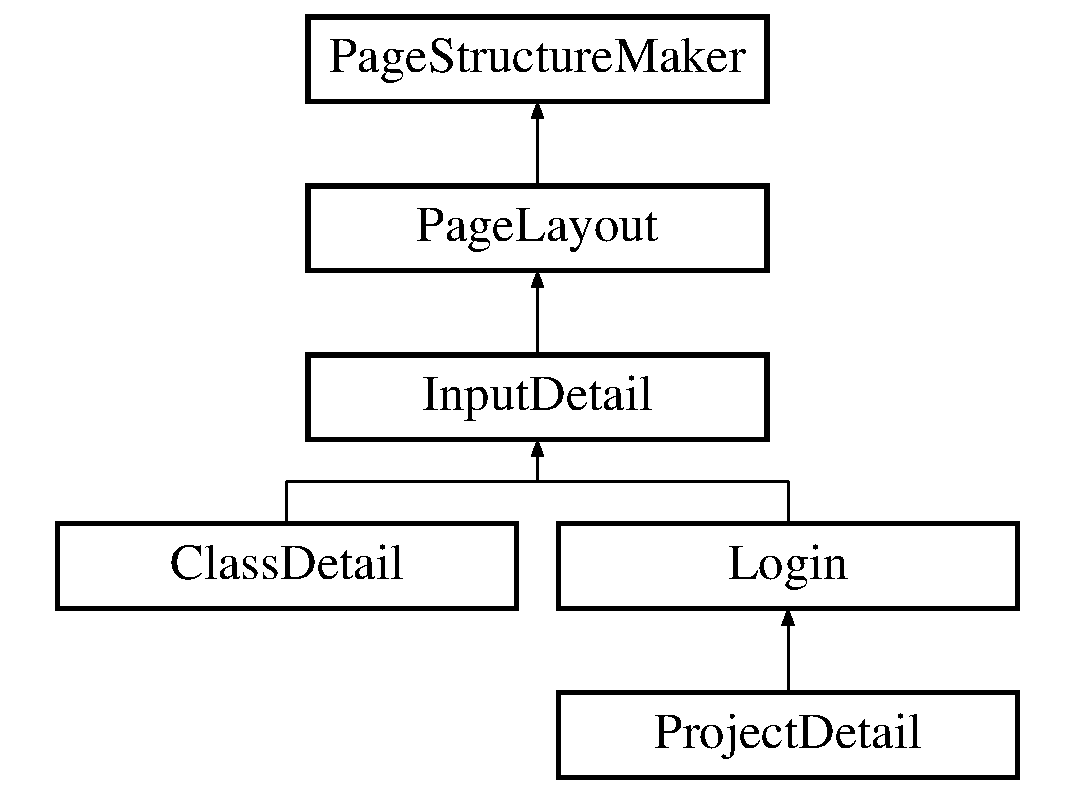
\includegraphics[height=2.000000cm]{classPageStructureMaker}
\end{center}
\end{figure}
\subsection*{Public Member Functions}
\begin{DoxyCompactItemize}
\item 
\hyperlink{classPageStructureMaker_a95e6305a2b5121840fb5b74297a040ce}{Page\-Structure\-Maker} ()
\item 
void \hyperlink{classPageStructureMaker_aaf78d67380c400cc0057c6519276f721}{Set\-H\-T\-M\-L\-Variables} ()
\item 
void \hyperlink{classPageStructureMaker_ad25d6abc983253567e2370882fc1b407}{H\-T\-M\-L\-Start} ()
\item 
void \hyperlink{classPageStructureMaker_a63b877af1c2c8de8332e3f7eb4c2c2b0}{H\-T\-M\-L\-End} ()
\item 
void \hyperlink{classPageStructureMaker_a14312134cb108f91f2e6d9cbd6916e97}{Head\-Start} ()
\item 
void \hyperlink{classPageStructureMaker_ad64115d592b0989b422a93f85278186e}{Head\-End} ()
\item 
void \hyperlink{classPageStructureMaker_a81e902ddc0c0287df1ba0f614a3774d6}{Title} (string page\-Title)
\item 
void \hyperlink{classPageStructureMaker_aacdb11817f8ab246bc59c552e04e862d}{C\-S\-S} (string href)
\item 
void \hyperlink{classPageStructureMaker_ac221d1169f4dbcef6adb00938919193d}{Javascript} (string src)
\item 
void \hyperlink{classPageStructureMaker_ab7a645675166f34fac99f1ed8feb7c27}{Body\-Start} ()
\item 
void \hyperlink{classPageStructureMaker_ac91e234e2d54dedd9d7e556fabf21d2b}{Body\-End} ()
\item 
void \hyperlink{classPageStructureMaker_a927f92889555dd316c129f706be86a5c}{Div\-Start} (string id, string class\-Name)
\item 
void \hyperlink{classPageStructureMaker_a2913e76bf188ed777dcd33003ef6207d}{Div\-End} ()
\item 
void \hyperlink{classPageStructureMaker_a3f25d5b844a2251883acb80d8fabb77d}{Form\-Start} (string name, string action, string method)
\item 
void \hyperlink{classPageStructureMaker_a65d97f23bb543f3db5201b2009f7f65a}{Form\-End} ()
\item 
void \hyperlink{classPageStructureMaker_a04e68e69005f3933e0f496c3db474daf}{Table\-Start} (string id, string class\-Name)
\item 
void \hyperlink{classPageStructureMaker_a7f8fefbe7a825c1b7761fc8a0f1bb8e4}{Table\-End} ()
\item 
void \hyperlink{classPageStructureMaker_ac24ce26202757aaa30402155daf8a3d0}{List\-Start} (string list\-Type)
\item 
void \hyperlink{classPageStructureMaker_a8578b1555ad2fc92a9efc7dbf7d1fe87}{List\-End} (string list\-Type)
\item 
void \hyperlink{classPageStructureMaker_adf4116e526026edc3c8a3bcf96a7e929}{List\-Item} (string list\-Item)
\item 
void \hyperlink{classPageStructureMaker_a8c0fae5b599182863066de56ae0cea42}{Anchor} (string href, string target)
\item 
void \hyperlink{classPageStructureMaker_aec87050d1230402d695290fe78c86f03}{Input\-Field} (string type, string name, string placeholder, string value=\char`\"{}\char`\"{})
\item 
void \hyperlink{classPageStructureMaker_af528f8da142cbc47585c4dfeded873ba}{Input\-Field} (string type, string name, int name\-No, string placeholder, string value=\char`\"{}\char`\"{})
\item 
void \hyperlink{classPageStructureMaker_ae85f66489db9a65682bb9a2c2128f433}{Label} (string for\-Field, string value)
\item 
void \hyperlink{classPageStructureMaker_ae8684bb66ca463e2f92e09c96137f9e3}{Select\-Field\-Start} (string name)
\item 
void \hyperlink{classPageStructureMaker_a81eb3cdbc840a4c8165cef87330ade09}{Select\-Field\-End} ()
\item 
void \hyperlink{classPageStructureMaker_a77856078e74dab25329132ea07466f92}{Select\-Option\-Start} (string value, string selected)
\item 
void \hyperlink{classPageStructureMaker_a7682f479f7f1012d426ec9f9535def60}{Select\-Option\-End} ()
\item 
void \hyperlink{classPageStructureMaker_a53c013b1d6251be853be8f6c413e3455}{Button} (string id, string type, string class\-Name, string value, string on\-Click=\char`\"{}\char`\"{})
\end{DoxyCompactItemize}
\subsection*{Public Attributes}
\begin{DoxyCompactItemize}
\item 
string \hyperlink{classPageStructureMaker_af41d4e21b808f5f8dc2c727f775b6fb2}{start\-H1}
\item 
\hypertarget{classPageStructureMaker_a3786a6f477632e4a60205a988d6b599d}{string {\bfseries end\-H1}}\label{classPageStructureMaker_a3786a6f477632e4a60205a988d6b599d}

\item 
\hypertarget{classPageStructureMaker_adb966c147c6328c8e48281c882de776d}{string {\bfseries start\-H3}}\label{classPageStructureMaker_adb966c147c6328c8e48281c882de776d}

\item 
\hypertarget{classPageStructureMaker_a22e6bf3eb787284b745d694613c1d9da}{string {\bfseries end\-H3}}\label{classPageStructureMaker_a22e6bf3eb787284b745d694613c1d9da}

\item 
\hypertarget{classPageStructureMaker_a7e458e675a3adf987a153e08f3795941}{string {\bfseries start\-T\-D}}\label{classPageStructureMaker_a7e458e675a3adf987a153e08f3795941}

\item 
\hypertarget{classPageStructureMaker_ad27f03939a04048a03be0f1bb8edd38a}{string {\bfseries end\-T\-D}}\label{classPageStructureMaker_ad27f03939a04048a03be0f1bb8edd38a}

\item 
\hypertarget{classPageStructureMaker_a4fe234b016efcb9eaa757879b8858190}{string {\bfseries start\-T\-H}}\label{classPageStructureMaker_a4fe234b016efcb9eaa757879b8858190}

\item 
\hypertarget{classPageStructureMaker_aa244b4ef71850dc76fcfb5157bcaf8fc}{string {\bfseries end\-T\-H}}\label{classPageStructureMaker_aa244b4ef71850dc76fcfb5157bcaf8fc}

\item 
\hypertarget{classPageStructureMaker_aa59b4949d26fab5a72710fa9fc3e8ea9}{string {\bfseries start\-T\-R}}\label{classPageStructureMaker_aa59b4949d26fab5a72710fa9fc3e8ea9}

\item 
\hypertarget{classPageStructureMaker_afee49ebdcbc0971142fcf7eae8baa306}{string {\bfseries end\-T\-R}}\label{classPageStructureMaker_afee49ebdcbc0971142fcf7eae8baa306}

\item 
\hypertarget{classPageStructureMaker_aa0f624b485f07f6e19151b1df3dc59a3}{string {\bfseries start\-B}}\label{classPageStructureMaker_aa0f624b485f07f6e19151b1df3dc59a3}

\item 
\hypertarget{classPageStructureMaker_ad46c3195310a1f0226e21d2eb5befb00}{string {\bfseries end\-B}}\label{classPageStructureMaker_ad46c3195310a1f0226e21d2eb5befb00}

\item 
\hypertarget{classPageStructureMaker_a63911cb925ccdc6c879905a677ed8881}{string {\bfseries brk}}\label{classPageStructureMaker_a63911cb925ccdc6c879905a677ed8881}

\end{DoxyCompactItemize}


\subsection{Detailed Description}
\subsection*{Include Header file }

Class\-: \hyperlink{classPageStructureMaker}{Page\-Structure\-Maker} \subsection*{Description\-: Declaration}

Definition at line 34 of file pagestructure.\-h.



\subsection{Constructor \& Destructor Documentation}
\hypertarget{classPageStructureMaker_a95e6305a2b5121840fb5b74297a040ce}{\index{Page\-Structure\-Maker@{Page\-Structure\-Maker}!Page\-Structure\-Maker@{Page\-Structure\-Maker}}
\index{Page\-Structure\-Maker@{Page\-Structure\-Maker}!PageStructureMaker@{Page\-Structure\-Maker}}
\subsubsection[{Page\-Structure\-Maker}]{\setlength{\rightskip}{0pt plus 5cm}Page\-Structure\-Maker\-::\-Page\-Structure\-Maker (
\begin{DoxyParamCaption}
{}
\end{DoxyParamCaption}
)}}\label{classPageStructureMaker_a95e6305a2b5121840fb5b74297a040ce}
Constructor



 \subsubsection*{Include htmltags.\-h header files}



 Class\-: \hyperlink{classPageStructureMaker}{Page\-Structure\-Maker} Method\-: \hyperlink{classPageStructureMaker}{Page\-Structure\-Maker} \-:\-: \hyperlink{classPageStructureMaker_a95e6305a2b5121840fb5b74297a040ce}{Page\-Structure\-Maker()} \subsubsection*{Description\-: Constructor}

Definition at line 33 of file pagestructure.\-cc.



\subsection{Member Function Documentation}
\hypertarget{classPageStructureMaker_a8c0fae5b599182863066de56ae0cea42}{\index{Page\-Structure\-Maker@{Page\-Structure\-Maker}!Anchor@{Anchor}}
\index{Anchor@{Anchor}!PageStructureMaker@{Page\-Structure\-Maker}}
\subsubsection[{Anchor}]{\setlength{\rightskip}{0pt plus 5cm}void Page\-Structure\-Maker\-::\-Anchor (
\begin{DoxyParamCaption}
\item[{string}]{href, }
\item[{string}]{target}
\end{DoxyParamCaption}
)}}\label{classPageStructureMaker_a8c0fae5b599182863066de56ae0cea42}
Anchor Tag

-\/-\/-\/-\/-\/-\/-\/-\/-\/-\/-\/-\/-\/-\/-\/-\/-\/-\/-\/-\/-\/-\/-\/-\/-\/-\/-\/-\/-\/-\/-\/-\/-\/-\/-\/-\/-\/-\/-\/-\/-\/-\/-\/-\/-\/-\/-\/-\/-\/-\/-\/-\/-\/-\/-\/-\/-\/-\/-\/-\/-\/-\/-\/-\/-\/---\par
 Class\-: \hyperlink{classPageStructureMaker}{Page\-Structure\-Maker} \par
 Method\-: \hyperlink{classPageStructureMaker}{Page\-Structure\-Maker} \-:\-: Anchor(string href) \par
 \subsubsection*{Description\-: Anchor Tag }

Definition at line 319 of file pagestructure.\-cc.

\hypertarget{classPageStructureMaker_ac91e234e2d54dedd9d7e556fabf21d2b}{\index{Page\-Structure\-Maker@{Page\-Structure\-Maker}!Body\-End@{Body\-End}}
\index{Body\-End@{Body\-End}!PageStructureMaker@{Page\-Structure\-Maker}}
\subsubsection[{Body\-End}]{\setlength{\rightskip}{0pt plus 5cm}void Page\-Structure\-Maker\-::\-Body\-End (
\begin{DoxyParamCaption}
{}
\end{DoxyParamCaption}
)}}\label{classPageStructureMaker_ac91e234e2d54dedd9d7e556fabf21d2b}
Display $<$/\-B\-O\-D\-Y$>$



 Class\-: \hyperlink{classPageStructureMaker}{Page\-Structure\-Maker} Method\-: \hyperlink{classPageStructureMaker}{Page\-Structure\-Maker} \-:\-: \hyperlink{classPageStructureMaker_ac91e234e2d54dedd9d7e556fabf21d2b}{Body\-End()} \subsubsection*{Description\-: Display $<$/\-B\-O\-D\-Y$>$}

Definition at line 180 of file pagestructure.\-cc.

\hypertarget{classPageStructureMaker_ab7a645675166f34fac99f1ed8feb7c27}{\index{Page\-Structure\-Maker@{Page\-Structure\-Maker}!Body\-Start@{Body\-Start}}
\index{Body\-Start@{Body\-Start}!PageStructureMaker@{Page\-Structure\-Maker}}
\subsubsection[{Body\-Start}]{\setlength{\rightskip}{0pt plus 5cm}void Page\-Structure\-Maker\-::\-Body\-Start (
\begin{DoxyParamCaption}
{}
\end{DoxyParamCaption}
)}}\label{classPageStructureMaker_ab7a645675166f34fac99f1ed8feb7c27}
Display $<$\-B\-O\-D\-Y$>$



 Class\-: \hyperlink{classPageStructureMaker}{Page\-Structure\-Maker} Method\-: \hyperlink{classPageStructureMaker}{Page\-Structure\-Maker} \-:\-: \hyperlink{classPageStructureMaker_ab7a645675166f34fac99f1ed8feb7c27}{Body\-Start()} \subsubsection*{Description\-: Display $<$B\-O\-D\-Y$>$}

Definition at line 166 of file pagestructure.\-cc.

\hypertarget{classPageStructureMaker_a53c013b1d6251be853be8f6c413e3455}{\index{Page\-Structure\-Maker@{Page\-Structure\-Maker}!Button@{Button}}
\index{Button@{Button}!PageStructureMaker@{Page\-Structure\-Maker}}
\subsubsection[{Button}]{\setlength{\rightskip}{0pt plus 5cm}void Page\-Structure\-Maker\-::\-Button (
\begin{DoxyParamCaption}
\item[{string}]{id, }
\item[{string}]{type, }
\item[{string}]{class\-Name, }
\item[{string}]{value, }
\item[{string}]{on\-Click = {\ttfamily \char`\"{}\char`\"{}}}
\end{DoxyParamCaption}
)}}\label{classPageStructureMaker_a53c013b1d6251be853be8f6c413e3455}
Button



 Class\-: \hyperlink{classPageStructureMaker}{Page\-Structure\-Maker} Method\-: \hyperlink{classPageStructureMaker}{Page\-Structure\-Maker} \-:\-: Button(string id, string type, string class\-Name, string value) \subsubsection*{Description\-: Create button(next, submit, etc)}

Definition at line 474 of file pagestructure.\-cc.

\hypertarget{classPageStructureMaker_aacdb11817f8ab246bc59c552e04e862d}{\index{Page\-Structure\-Maker@{Page\-Structure\-Maker}!C\-S\-S@{C\-S\-S}}
\index{C\-S\-S@{C\-S\-S}!PageStructureMaker@{Page\-Structure\-Maker}}
\subsubsection[{C\-S\-S}]{\setlength{\rightskip}{0pt plus 5cm}void Page\-Structure\-Maker\-::\-C\-S\-S (
\begin{DoxyParamCaption}
\item[{string}]{href}
\end{DoxyParamCaption}
)}}\label{classPageStructureMaker_aacdb11817f8ab246bc59c552e04e862d}
Add External C\-S\-S



 Class\-: \hyperlink{classPageStructureMaker}{Page\-Structure\-Maker} Method\-: \hyperlink{classPageStructureMaker}{Page\-Structure\-Maker} \-:\-: \hyperlink{classPageStructureMaker_aacdb11817f8ab246bc59c552e04e862d}{C\-S\-S(string href)} \subsubsection*{Description\-: Add External C\-S\-S file}

Definition at line 138 of file pagestructure.\-cc.

\hypertarget{classPageStructureMaker_a2913e76bf188ed777dcd33003ef6207d}{\index{Page\-Structure\-Maker@{Page\-Structure\-Maker}!Div\-End@{Div\-End}}
\index{Div\-End@{Div\-End}!PageStructureMaker@{Page\-Structure\-Maker}}
\subsubsection[{Div\-End}]{\setlength{\rightskip}{0pt plus 5cm}void Page\-Structure\-Maker\-::\-Div\-End (
\begin{DoxyParamCaption}
{}
\end{DoxyParamCaption}
)}}\label{classPageStructureMaker_a2913e76bf188ed777dcd33003ef6207d}
End div section



 Class\-: \hyperlink{classPageStructureMaker}{Page\-Structure\-Maker} Method\-: \hyperlink{classPageStructureMaker}{Page\-Structure\-Maker} \-:\-: \hyperlink{classPageStructureMaker_a2913e76bf188ed777dcd33003ef6207d}{Div\-End()} \subsubsection*{Description\-: Close Div Section}

Definition at line 209 of file pagestructure.\-cc.

\hypertarget{classPageStructureMaker_a927f92889555dd316c129f706be86a5c}{\index{Page\-Structure\-Maker@{Page\-Structure\-Maker}!Div\-Start@{Div\-Start}}
\index{Div\-Start@{Div\-Start}!PageStructureMaker@{Page\-Structure\-Maker}}
\subsubsection[{Div\-Start}]{\setlength{\rightskip}{0pt plus 5cm}void Page\-Structure\-Maker\-::\-Div\-Start (
\begin{DoxyParamCaption}
\item[{string}]{id, }
\item[{string}]{class\-Name}
\end{DoxyParamCaption}
)}}\label{classPageStructureMaker_a927f92889555dd316c129f706be86a5c}
Start Div Section



 Class\-: \hyperlink{classPageStructureMaker}{Page\-Structure\-Maker} Method\-: \hyperlink{classPageStructureMaker}{Page\-Structure\-Maker} \-:\-: Div\-Start(string id, string class\-Name) \subsubsection*{Description\-: Start Div Section with id and class\-Name(for C\-S\-S)}

Definition at line 195 of file pagestructure.\-cc.

\hypertarget{classPageStructureMaker_a65d97f23bb543f3db5201b2009f7f65a}{\index{Page\-Structure\-Maker@{Page\-Structure\-Maker}!Form\-End@{Form\-End}}
\index{Form\-End@{Form\-End}!PageStructureMaker@{Page\-Structure\-Maker}}
\subsubsection[{Form\-End}]{\setlength{\rightskip}{0pt plus 5cm}void Page\-Structure\-Maker\-::\-Form\-End (
\begin{DoxyParamCaption}
{}
\end{DoxyParamCaption}
)}}\label{classPageStructureMaker_a65d97f23bb543f3db5201b2009f7f65a}
End Form



 Class\-: \hyperlink{classPageStructureMaker}{Page\-Structure\-Maker} Method\-: \hyperlink{classPageStructureMaker}{Page\-Structure\-Maker} \-:\-: \hyperlink{classPageStructureMaker_a65d97f23bb543f3db5201b2009f7f65a}{Form\-End()} \subsubsection*{Description\-: Close Form}

Definition at line 239 of file pagestructure.\-cc.

\hypertarget{classPageStructureMaker_a3f25d5b844a2251883acb80d8fabb77d}{\index{Page\-Structure\-Maker@{Page\-Structure\-Maker}!Form\-Start@{Form\-Start}}
\index{Form\-Start@{Form\-Start}!PageStructureMaker@{Page\-Structure\-Maker}}
\subsubsection[{Form\-Start}]{\setlength{\rightskip}{0pt plus 5cm}void Page\-Structure\-Maker\-::\-Form\-Start (
\begin{DoxyParamCaption}
\item[{string}]{name, }
\item[{string}]{action, }
\item[{string}]{method}
\end{DoxyParamCaption}
)}}\label{classPageStructureMaker_a3f25d5b844a2251883acb80d8fabb77d}
Start Form



 Class\-: \hyperlink{classPageStructureMaker}{Page\-Structure\-Maker} Method\-: \hyperlink{classPageStructureMaker}{Page\-Structure\-Maker} \-:\-: Form\-Start(string name, string action, string method) \subsubsection*{Description\-: Start Form with name, action and method(G\-E\-T/\-P\-O\-S\-T)}

Definition at line 223 of file pagestructure.\-cc.

\hypertarget{classPageStructureMaker_ad64115d592b0989b422a93f85278186e}{\index{Page\-Structure\-Maker@{Page\-Structure\-Maker}!Head\-End@{Head\-End}}
\index{Head\-End@{Head\-End}!PageStructureMaker@{Page\-Structure\-Maker}}
\subsubsection[{Head\-End}]{\setlength{\rightskip}{0pt plus 5cm}void Page\-Structure\-Maker\-::\-Head\-End (
\begin{DoxyParamCaption}
{}
\end{DoxyParamCaption}
)}}\label{classPageStructureMaker_ad64115d592b0989b422a93f85278186e}
Display $<$/\-H\-E\-A\-D$>$



 Class\-: \hyperlink{classPageStructureMaker}{Page\-Structure\-Maker} Method\-: \hyperlink{classPageStructureMaker}{Page\-Structure\-Maker} \-:\-: \hyperlink{classPageStructureMaker_ad64115d592b0989b422a93f85278186e}{Head\-End()} \subsubsection*{Description\-: Display $<$/\-H\-E\-A\-D$>$}

Definition at line 112 of file pagestructure.\-cc.

\hypertarget{classPageStructureMaker_a14312134cb108f91f2e6d9cbd6916e97}{\index{Page\-Structure\-Maker@{Page\-Structure\-Maker}!Head\-Start@{Head\-Start}}
\index{Head\-Start@{Head\-Start}!PageStructureMaker@{Page\-Structure\-Maker}}
\subsubsection[{Head\-Start}]{\setlength{\rightskip}{0pt plus 5cm}void Page\-Structure\-Maker\-::\-Head\-Start (
\begin{DoxyParamCaption}
{}
\end{DoxyParamCaption}
)}}\label{classPageStructureMaker_a14312134cb108f91f2e6d9cbd6916e97}
Display $<$\-H\-E\-A\-D$>$



 Class\-: \hyperlink{classPageStructureMaker}{Page\-Structure\-Maker} Method\-: \hyperlink{classPageStructureMaker}{Page\-Structure\-Maker} \-:\-: \hyperlink{classPageStructureMaker_a14312134cb108f91f2e6d9cbd6916e97}{Head\-Start()} \subsubsection*{Description\-: Display $<$H\-E\-A\-D$>$}

Definition at line 99 of file pagestructure.\-cc.

\hypertarget{classPageStructureMaker_a63b877af1c2c8de8332e3f7eb4c2c2b0}{\index{Page\-Structure\-Maker@{Page\-Structure\-Maker}!H\-T\-M\-L\-End@{H\-T\-M\-L\-End}}
\index{H\-T\-M\-L\-End@{H\-T\-M\-L\-End}!PageStructureMaker@{Page\-Structure\-Maker}}
\subsubsection[{H\-T\-M\-L\-End}]{\setlength{\rightskip}{0pt plus 5cm}void Page\-Structure\-Maker\-::\-H\-T\-M\-L\-End (
\begin{DoxyParamCaption}
{}
\end{DoxyParamCaption}
)}}\label{classPageStructureMaker_a63b877af1c2c8de8332e3f7eb4c2c2b0}
Display $<$/\-H\-T\-M\-L$>$



 Class\-: \hyperlink{classPageStructureMaker}{Page\-Structure\-Maker} Method\-: \hyperlink{classPageStructureMaker}{Page\-Structure\-Maker} \-:\-: \hyperlink{classPageStructureMaker_a63b877af1c2c8de8332e3f7eb4c2c2b0}{H\-T\-M\-L\-End()} \subsubsection*{Description\-: Display $<$/\-H\-T\-M\-L$>$}

Definition at line 86 of file pagestructure.\-cc.

\hypertarget{classPageStructureMaker_ad25d6abc983253567e2370882fc1b407}{\index{Page\-Structure\-Maker@{Page\-Structure\-Maker}!H\-T\-M\-L\-Start@{H\-T\-M\-L\-Start}}
\index{H\-T\-M\-L\-Start@{H\-T\-M\-L\-Start}!PageStructureMaker@{Page\-Structure\-Maker}}
\subsubsection[{H\-T\-M\-L\-Start}]{\setlength{\rightskip}{0pt plus 5cm}void Page\-Structure\-Maker\-::\-H\-T\-M\-L\-Start (
\begin{DoxyParamCaption}
{}
\end{DoxyParamCaption}
)}}\label{classPageStructureMaker_ad25d6abc983253567e2370882fc1b407}
Display $<$\-H\-T\-M\-L$>$



 Class\-: \hyperlink{classPageStructureMaker}{Page\-Structure\-Maker} Method\-: \hyperlink{classPageStructureMaker}{Page\-Structure\-Maker} \-:\-: \hyperlink{classPageStructureMaker_ad25d6abc983253567e2370882fc1b407}{H\-T\-M\-L\-Start()} \subsubsection*{Description\-: Display $<$H\-T\-M\-L$>$ Tag }

Definition at line 73 of file pagestructure.\-cc.

\hypertarget{classPageStructureMaker_aec87050d1230402d695290fe78c86f03}{\index{Page\-Structure\-Maker@{Page\-Structure\-Maker}!Input\-Field@{Input\-Field}}
\index{Input\-Field@{Input\-Field}!PageStructureMaker@{Page\-Structure\-Maker}}
\subsubsection[{Input\-Field}]{\setlength{\rightskip}{0pt plus 5cm}void Page\-Structure\-Maker\-::\-Input\-Field (
\begin{DoxyParamCaption}
\item[{string}]{type, }
\item[{string}]{name, }
\item[{string}]{placeholder, }
\item[{string}]{value = {\ttfamily \char`\"{}\char`\"{}}}
\end{DoxyParamCaption}
)}}\label{classPageStructureMaker_aec87050d1230402d695290fe78c86f03}
Input field with 3 arguments

-\/-\/-\/-\/-\/-\/-\/-\/-\/-\/-\/-\/-\/-\/-\/-\/-\/-\/-\/-\/-\/-\/-\/-\/-\/-\/-\/-\/-\/-\/-\/-\/-\/-\/-\/-\/-\/-\/-\/-\/-\/-\/-\/-\/-\/-\/-\/-\/-\/-\/-\/-\/-\/-\/-\/-\/-\/-\/-\/-\/-\/-\/-\/-\/-\/---\par
 Class\-: \hyperlink{classPageStructureMaker}{Page\-Structure\-Maker} \par
 Method\-: \hyperlink{classPageStructureMaker}{Page\-Structure\-Maker} \-:\-: Input\-Field(string type, string name, string value) \par
 \subsubsection*{Description\-: For creating input field with 3 arguments }

Definition at line 348 of file pagestructure.\-cc.

\hypertarget{classPageStructureMaker_af528f8da142cbc47585c4dfeded873ba}{\index{Page\-Structure\-Maker@{Page\-Structure\-Maker}!Input\-Field@{Input\-Field}}
\index{Input\-Field@{Input\-Field}!PageStructureMaker@{Page\-Structure\-Maker}}
\subsubsection[{Input\-Field}]{\setlength{\rightskip}{0pt plus 5cm}void Page\-Structure\-Maker\-::\-Input\-Field (
\begin{DoxyParamCaption}
\item[{string}]{type, }
\item[{string}]{name, }
\item[{int}]{name\-No, }
\item[{string}]{placeholder, }
\item[{string}]{value = {\ttfamily \char`\"{}\char`\"{}}}
\end{DoxyParamCaption}
)}}\label{classPageStructureMaker_af528f8da142cbc47585c4dfeded873ba}
Input Field with 4 arguments



 Class\-: \hyperlink{classPageStructureMaker}{Page\-Structure\-Maker} Method\-: \hyperlink{classPageStructureMaker}{Page\-Structure\-Maker} \-:\-: Input\-Field(string type, string name, string value) Description\-: Create Input fields like text field, submit \subsubsection*{button, etc.}

Definition at line 386 of file pagestructure.\-cc.

\hypertarget{classPageStructureMaker_ac221d1169f4dbcef6adb00938919193d}{\index{Page\-Structure\-Maker@{Page\-Structure\-Maker}!Javascript@{Javascript}}
\index{Javascript@{Javascript}!PageStructureMaker@{Page\-Structure\-Maker}}
\subsubsection[{Javascript}]{\setlength{\rightskip}{0pt plus 5cm}void Page\-Structure\-Maker\-::\-Javascript (
\begin{DoxyParamCaption}
\item[{string}]{src}
\end{DoxyParamCaption}
)}}\label{classPageStructureMaker_ac221d1169f4dbcef6adb00938919193d}
Add Javascript File



 Class\-: \hyperlink{classPageStructureMaker}{Page\-Structure\-Maker} Method\-: \hyperlink{classPageStructureMaker}{Page\-Structure\-Maker} \-:\-: \hyperlink{classPageStructureMaker_ac221d1169f4dbcef6adb00938919193d}{Javascript(string src)} \subsubsection*{Description\-: Add external Javascript file}

Definition at line 153 of file pagestructure.\-cc.

\hypertarget{classPageStructureMaker_ae85f66489db9a65682bb9a2c2128f433}{\index{Page\-Structure\-Maker@{Page\-Structure\-Maker}!Label@{Label}}
\index{Label@{Label}!PageStructureMaker@{Page\-Structure\-Maker}}
\subsubsection[{Label}]{\setlength{\rightskip}{0pt plus 5cm}void Page\-Structure\-Maker\-::\-Label (
\begin{DoxyParamCaption}
\item[{string}]{for\-Field, }
\item[{string}]{value}
\end{DoxyParamCaption}
)}}\label{classPageStructureMaker_ae85f66489db9a65682bb9a2c2128f433}
Label tag

-\/-\/-\/-\/-\/-\/-\/-\/-\/-\/-\/-\/-\/-\/-\/-\/-\/-\/-\/-\/-\/-\/-\/-\/-\/-\/-\/-\/-\/-\/-\/-\/-\/-\/-\/-\/-\/-\/-\/-\/-\/-\/-\/-\/-\/-\/-\/-\/-\/-\/-\/-\/-\/-\/-\/-\/-\/-\/-\/-\/-\/-\/-\/-\/-\/---\par
 Class\-: \hyperlink{classPageStructureMaker}{Page\-Structure\-Maker} \par
 Method\-: \hyperlink{classPageStructureMaker}{Page\-Structure\-Maker} \-:\-: Label(string for\-Value, string value) \par
 \subsubsection*{Description\-: For adding label in html page }

Definition at line 333 of file pagestructure.\-cc.

\hypertarget{classPageStructureMaker_a8578b1555ad2fc92a9efc7dbf7d1fe87}{\index{Page\-Structure\-Maker@{Page\-Structure\-Maker}!List\-End@{List\-End}}
\index{List\-End@{List\-End}!PageStructureMaker@{Page\-Structure\-Maker}}
\subsubsection[{List\-End}]{\setlength{\rightskip}{0pt plus 5cm}void Page\-Structure\-Maker\-::\-List\-End (
\begin{DoxyParamCaption}
\item[{string}]{list\-Type}
\end{DoxyParamCaption}
)}}\label{classPageStructureMaker_a8578b1555ad2fc92a9efc7dbf7d1fe87}
End List

-\/-\/-\/-\/-\/-\/-\/-\/-\/-\/-\/-\/-\/-\/-\/-\/-\/-\/-\/-\/-\/-\/-\/-\/-\/-\/-\/-\/-\/-\/-\/-\/-\/-\/-\/-\/-\/-\/-\/-\/-\/-\/-\/-\/-\/-\/-\/-\/-\/-\/-\/-\/-\/-\/-\/-\/-\/-\/-\/-\/-\/-\/-\/-\/-\/---\par
 Class\-: \hyperlink{classPageStructureMaker}{Page\-Structure\-Maker} \par
 Method\-: \hyperlink{classPageStructureMaker}{Page\-Structure\-Maker} \-:\-: \hyperlink{classPageStructureMaker_a8578b1555ad2fc92a9efc7dbf7d1fe87}{List\-End(string list\-Type)} \par
 \subsubsection*{Description\-: Close List Tag }

Definition at line 293 of file pagestructure.\-cc.

\hypertarget{classPageStructureMaker_adf4116e526026edc3c8a3bcf96a7e929}{\index{Page\-Structure\-Maker@{Page\-Structure\-Maker}!List\-Item@{List\-Item}}
\index{List\-Item@{List\-Item}!PageStructureMaker@{Page\-Structure\-Maker}}
\subsubsection[{List\-Item}]{\setlength{\rightskip}{0pt plus 5cm}void Page\-Structure\-Maker\-::\-List\-Item (
\begin{DoxyParamCaption}
\item[{string}]{list\-Item}
\end{DoxyParamCaption}
)}}\label{classPageStructureMaker_adf4116e526026edc3c8a3bcf96a7e929}
List Item

-\/-\/-\/-\/-\/-\/-\/-\/-\/-\/-\/-\/-\/-\/-\/-\/-\/-\/-\/-\/-\/-\/-\/-\/-\/-\/-\/-\/-\/-\/-\/-\/-\/-\/-\/-\/-\/-\/-\/-\/-\/-\/-\/-\/-\/-\/-\/-\/-\/-\/-\/-\/-\/-\/-\/-\/-\/-\/-\/-\/-\/-\/-\/-\/-\/---\par
 Class\-: \hyperlink{classPageStructureMaker}{Page\-Structure\-Maker} \par
 Method\-: \hyperlink{classPageStructureMaker}{Page\-Structure\-Maker} \-:\-: \hyperlink{classPageStructureMaker_adf4116e526026edc3c8a3bcf96a7e929}{List\-Item(string list\-Item)} \par
 \subsubsection*{Description\-: List Item }

Definition at line 306 of file pagestructure.\-cc.

\hypertarget{classPageStructureMaker_ac24ce26202757aaa30402155daf8a3d0}{\index{Page\-Structure\-Maker@{Page\-Structure\-Maker}!List\-Start@{List\-Start}}
\index{List\-Start@{List\-Start}!PageStructureMaker@{Page\-Structure\-Maker}}
\subsubsection[{List\-Start}]{\setlength{\rightskip}{0pt plus 5cm}void Page\-Structure\-Maker\-::\-List\-Start (
\begin{DoxyParamCaption}
\item[{string}]{list\-Type}
\end{DoxyParamCaption}
)}}\label{classPageStructureMaker_ac24ce26202757aaa30402155daf8a3d0}
Start List

-\/-\/-\/-\/-\/-\/-\/-\/-\/-\/-\/-\/-\/-\/-\/-\/-\/-\/-\/-\/-\/-\/-\/-\/-\/-\/-\/-\/-\/-\/-\/-\/-\/-\/-\/-\/-\/-\/-\/-\/-\/-\/-\/-\/-\/-\/-\/-\/-\/-\/-\/-\/-\/-\/-\/-\/-\/-\/-\/-\/-\/-\/-\/-\/-\/---\par
 Class\-: \hyperlink{classPageStructureMaker}{Page\-Structure\-Maker} \par
 Method\-: \hyperlink{classPageStructureMaker}{Page\-Structure\-Maker} \-:\-: \hyperlink{classPageStructureMaker_ac24ce26202757aaa30402155daf8a3d0}{List\-Start(string list\-Type)} \par
 \subsubsection*{Description\-: Start any list like ul, ol, etc. }

Definition at line 280 of file pagestructure.\-cc.

\hypertarget{classPageStructureMaker_a81eb3cdbc840a4c8165cef87330ade09}{\index{Page\-Structure\-Maker@{Page\-Structure\-Maker}!Select\-Field\-End@{Select\-Field\-End}}
\index{Select\-Field\-End@{Select\-Field\-End}!PageStructureMaker@{Page\-Structure\-Maker}}
\subsubsection[{Select\-Field\-End}]{\setlength{\rightskip}{0pt plus 5cm}void Page\-Structure\-Maker\-::\-Select\-Field\-End (
\begin{DoxyParamCaption}
{}
\end{DoxyParamCaption}
)}}\label{classPageStructureMaker_a81eb3cdbc840a4c8165cef87330ade09}
End Select Field



 Class\-: \hyperlink{classPageStructureMaker}{Page\-Structure\-Maker} Method\-: \hyperlink{classPageStructureMaker}{Page\-Structure\-Maker} \-:\-: \hyperlink{classPageStructureMaker_a81eb3cdbc840a4c8165cef87330ade09}{Select\-Field\-End()} \subsubsection*{Description\-: Close select field}

Definition at line 430 of file pagestructure.\-cc.

\hypertarget{classPageStructureMaker_ae8684bb66ca463e2f92e09c96137f9e3}{\index{Page\-Structure\-Maker@{Page\-Structure\-Maker}!Select\-Field\-Start@{Select\-Field\-Start}}
\index{Select\-Field\-Start@{Select\-Field\-Start}!PageStructureMaker@{Page\-Structure\-Maker}}
\subsubsection[{Select\-Field\-Start}]{\setlength{\rightskip}{0pt plus 5cm}void Page\-Structure\-Maker\-::\-Select\-Field\-Start (
\begin{DoxyParamCaption}
\item[{string}]{name}
\end{DoxyParamCaption}
)}}\label{classPageStructureMaker_ae8684bb66ca463e2f92e09c96137f9e3}
Select Field Start



 Class\-: \hyperlink{classPageStructureMaker}{Page\-Structure\-Maker} Method\-: \hyperlink{classPageStructureMaker}{Page\-Structure\-Maker} \-:\-: \hyperlink{classPageStructureMaker_ae8684bb66ca463e2f92e09c96137f9e3}{Select\-Field\-Start(string name)} \subsubsection*{Description\-: Create Select Field}

Definition at line 417 of file pagestructure.\-cc.

\hypertarget{classPageStructureMaker_a7682f479f7f1012d426ec9f9535def60}{\index{Page\-Structure\-Maker@{Page\-Structure\-Maker}!Select\-Option\-End@{Select\-Option\-End}}
\index{Select\-Option\-End@{Select\-Option\-End}!PageStructureMaker@{Page\-Structure\-Maker}}
\subsubsection[{Select\-Option\-End}]{\setlength{\rightskip}{0pt plus 5cm}void Page\-Structure\-Maker\-::\-Select\-Option\-End (
\begin{DoxyParamCaption}
{}
\end{DoxyParamCaption}
)}}\label{classPageStructureMaker_a7682f479f7f1012d426ec9f9535def60}
Selct Option End



 Class\-: \hyperlink{classPageStructureMaker}{Page\-Structure\-Maker} Method\-: \hyperlink{classPageStructureMaker}{Page\-Structure\-Maker} \-:\-: \hyperlink{classPageStructureMaker_a7682f479f7f1012d426ec9f9535def60}{Select\-Option\-End()} \subsubsection*{Description\-: Close select option}

Definition at line 460 of file pagestructure.\-cc.

\hypertarget{classPageStructureMaker_a77856078e74dab25329132ea07466f92}{\index{Page\-Structure\-Maker@{Page\-Structure\-Maker}!Select\-Option\-Start@{Select\-Option\-Start}}
\index{Select\-Option\-Start@{Select\-Option\-Start}!PageStructureMaker@{Page\-Structure\-Maker}}
\subsubsection[{Select\-Option\-Start}]{\setlength{\rightskip}{0pt plus 5cm}void Page\-Structure\-Maker\-::\-Select\-Option\-Start (
\begin{DoxyParamCaption}
\item[{string}]{value, }
\item[{string}]{selected}
\end{DoxyParamCaption}
)}}\label{classPageStructureMaker_a77856078e74dab25329132ea07466f92}
Select Option Start



 Class\-: \hyperlink{classPageStructureMaker}{Page\-Structure\-Maker} Method\-: \hyperlink{classPageStructureMaker}{Page\-Structure\-Maker} \-:\-: Select\-Option\-Start(string value, string selected) \subsubsection*{Description\-: Options for select }

Definition at line 444 of file pagestructure.\-cc.

\hypertarget{classPageStructureMaker_aaf78d67380c400cc0057c6519276f721}{\index{Page\-Structure\-Maker@{Page\-Structure\-Maker}!Set\-H\-T\-M\-L\-Variables@{Set\-H\-T\-M\-L\-Variables}}
\index{Set\-H\-T\-M\-L\-Variables@{Set\-H\-T\-M\-L\-Variables}!PageStructureMaker@{Page\-Structure\-Maker}}
\subsubsection[{Set\-H\-T\-M\-L\-Variables}]{\setlength{\rightskip}{0pt plus 5cm}void Page\-Structure\-Maker\-::\-Set\-H\-T\-M\-L\-Variables (
\begin{DoxyParamCaption}
{}
\end{DoxyParamCaption}
)}}\label{classPageStructureMaker_aaf78d67380c400cc0057c6519276f721}
Assingn Values to variables



 Class\-: \hyperlink{classPageStructureMaker}{Page\-Structure\-Maker} Method\-: \hyperlink{classPageStructureMaker}{Page\-Structure\-Maker} \-:\-: \hyperlink{classPageStructureMaker_aaf78d67380c400cc0057c6519276f721}{Set\-H\-T\-M\-L\-Variables()} Description\-: Set values of common H\-T\-M\-L tags in respective \subsubsection*{variables.}

Definition at line 48 of file pagestructure.\-cc.

\hypertarget{classPageStructureMaker_a7f8fefbe7a825c1b7761fc8a0f1bb8e4}{\index{Page\-Structure\-Maker@{Page\-Structure\-Maker}!Table\-End@{Table\-End}}
\index{Table\-End@{Table\-End}!PageStructureMaker@{Page\-Structure\-Maker}}
\subsubsection[{Table\-End}]{\setlength{\rightskip}{0pt plus 5cm}void Page\-Structure\-Maker\-::\-Table\-End (
\begin{DoxyParamCaption}
{}
\end{DoxyParamCaption}
)}}\label{classPageStructureMaker_a7f8fefbe7a825c1b7761fc8a0f1bb8e4}
End Table



 Class\-: \hyperlink{classPageStructureMaker}{Page\-Structure\-Maker} Method\-: \hyperlink{classPageStructureMaker}{Page\-Structure\-Maker} \-:\-: \hyperlink{classPageStructureMaker_a7f8fefbe7a825c1b7761fc8a0f1bb8e4}{Table\-End()} \subsubsection*{Description\-: Close Table tag}

Definition at line 267 of file pagestructure.\-cc.

\hypertarget{classPageStructureMaker_a04e68e69005f3933e0f496c3db474daf}{\index{Page\-Structure\-Maker@{Page\-Structure\-Maker}!Table\-Start@{Table\-Start}}
\index{Table\-Start@{Table\-Start}!PageStructureMaker@{Page\-Structure\-Maker}}
\subsubsection[{Table\-Start}]{\setlength{\rightskip}{0pt plus 5cm}void Page\-Structure\-Maker\-::\-Table\-Start (
\begin{DoxyParamCaption}
\item[{string}]{id, }
\item[{string}]{class\-Name}
\end{DoxyParamCaption}
)}}\label{classPageStructureMaker_a04e68e69005f3933e0f496c3db474daf}
Start Table



 Class\-: \hyperlink{classPageStructureMaker}{Page\-Structure\-Maker} Method\-: \hyperlink{classPageStructureMaker}{Page\-Structure\-Maker} \-:\-: Table\-Start(string id, string class\-Name) \subsubsection*{Description\-: Start Table with id and class\-Name(\-C\-S\-S) attributes}

Definition at line 253 of file pagestructure.\-cc.

\hypertarget{classPageStructureMaker_a81e902ddc0c0287df1ba0f614a3774d6}{\index{Page\-Structure\-Maker@{Page\-Structure\-Maker}!Title@{Title}}
\index{Title@{Title}!PageStructureMaker@{Page\-Structure\-Maker}}
\subsubsection[{Title}]{\setlength{\rightskip}{0pt plus 5cm}void Page\-Structure\-Maker\-::\-Title (
\begin{DoxyParamCaption}
\item[{string}]{page\-Title}
\end{DoxyParamCaption}
)}}\label{classPageStructureMaker_a81e902ddc0c0287df1ba0f614a3774d6}
Display $<$\-T\-I\-T\-L\-E$>$ $<$/\-T\-I\-T\-L\-E$>$



 Class\-: \hyperlink{classPageStructureMaker}{Page\-Structure\-Maker} Method\-: \hyperlink{classPageStructureMaker}{Page\-Structure\-Maker} \-:\-: \hyperlink{classPageStructureMaker_a81e902ddc0c0287df1ba0f614a3774d6}{Title(string page\-Title)} \subsubsection*{Description\-: Display Page Tile}

Definition at line 125 of file pagestructure.\-cc.



\subsection{Member Data Documentation}
\hypertarget{classPageStructureMaker_af41d4e21b808f5f8dc2c727f775b6fb2}{\index{Page\-Structure\-Maker@{Page\-Structure\-Maker}!start\-H1@{start\-H1}}
\index{start\-H1@{start\-H1}!PageStructureMaker@{Page\-Structure\-Maker}}
\subsubsection[{start\-H1}]{\setlength{\rightskip}{0pt plus 5cm}string Page\-Structure\-Maker\-::start\-H1}}\label{classPageStructureMaker_af41d4e21b808f5f8dc2c727f775b6fb2}
H\-T\-M\-L Tag Variables for td, th, bold, etc 

Definition at line 38 of file pagestructure.\-h.



The documentation for this class was generated from the following files\-:\begin{DoxyCompactItemize}
\item 
src/header/pagestructure.\-h\item 
src/pagestructure.\-cc\end{DoxyCompactItemize}

\hypertarget{classProjectDetail}{\section{Project\-Detail Class Reference}
\label{classProjectDetail}\index{Project\-Detail@{Project\-Detail}}
}


\hyperlink{classProjectDetail}{Project\-Detail} class for creating new project for user.  




{\ttfamily \#include $<$project.\-h$>$}

Inheritance diagram for Project\-Detail\-:\begin{figure}[H]
\begin{center}
\leavevmode
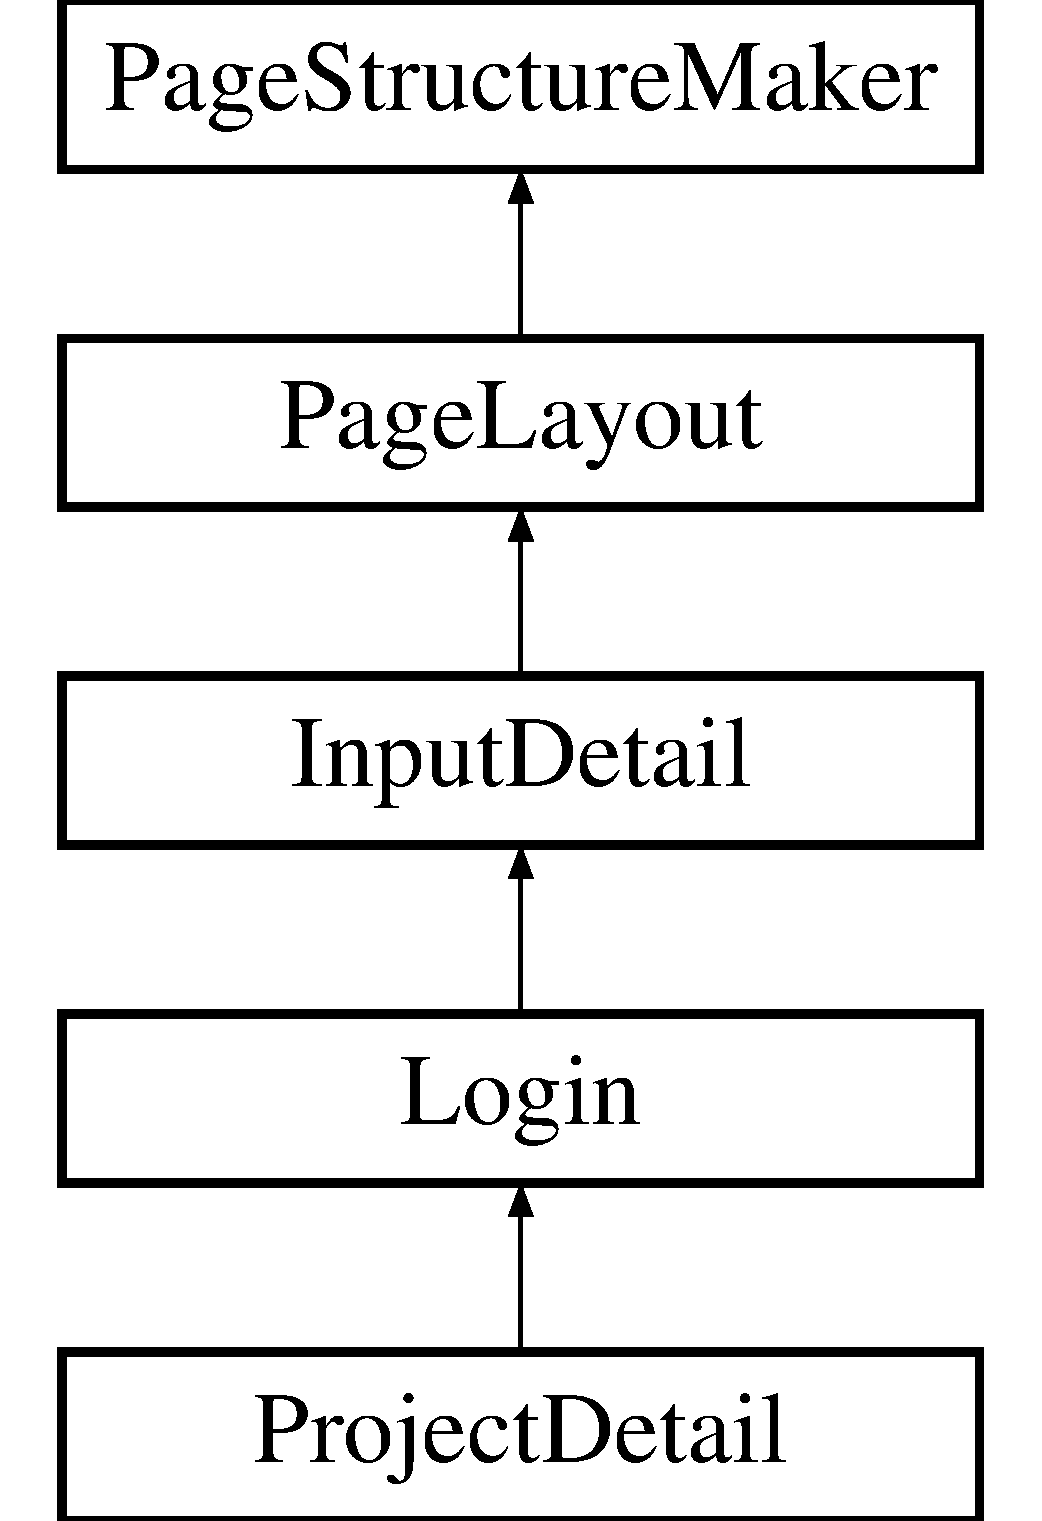
\includegraphics[height=3.000000cm]{classProjectDetail}
\end{center}
\end{figure}
\subsection*{Public Member Functions}
\begin{DoxyCompactItemize}
\item 
\hyperlink{classProjectDetail_a405e8bbc157e30c4ff93871988218d9f}{Project\-Detail} ()
\item 
void \hyperlink{classProjectDetail_a581ccdab5dcd21663b78ebedbbf0d240}{Project\-Detail\-Page} (string \hyperlink{classInputDetail_a1abb16cd695678c3fa05e3c812823fee}{msg}=\char`\"{}\char`\"{}, string project\-Name=\char`\"{}Project Name\char`\"{})
\item 
void \hyperlink{classProjectDetail_ab78c9e2a0cd5079c427638a5a3971c28}{Authorize\-User} ()
\item 
\hypertarget{classProjectDetail_ab92c992a37524a5f90fdcaf4868ac218}{void \hyperlink{classProjectDetail_ab92c992a37524a5f90fdcaf4868ac218}{Old\-Project} ()}\label{classProjectDetail_ab92c992a37524a5f90fdcaf4868ac218}

\begin{DoxyCompactList}\small\item\em List Existing projects from database. \end{DoxyCompactList}\item 
\hypertarget{classProjectDetail_aa36fe7134da17688018870ae8ebf2191}{void \hyperlink{classProjectDetail_aa36fe7134da17688018870ae8ebf2191}{Home\-Page} ()}\label{classProjectDetail_aa36fe7134da17688018870ae8ebf2191}

\begin{DoxyCompactList}\small\item\em Home Page. \end{DoxyCompactList}\item 
\hyperlink{classProjectDetail_ab4719d14d9efb8811916f5d691099c8f}{$\sim$\-Project\-Detail} ()
\end{DoxyCompactItemize}
\subsection*{Additional Inherited Members}


\subsection{Detailed Description}
\hyperlink{classProjectDetail}{Project\-Detail} class for creating new project for user. 

Definition at line 28 of file project.\-h.



\subsection{Constructor \& Destructor Documentation}
\hypertarget{classProjectDetail_a405e8bbc157e30c4ff93871988218d9f}{\index{Project\-Detail@{Project\-Detail}!Project\-Detail@{Project\-Detail}}
\index{Project\-Detail@{Project\-Detail}!ProjectDetail@{Project\-Detail}}
\subsubsection[{Project\-Detail}]{\setlength{\rightskip}{0pt plus 5cm}Project\-Detail\-::\-Project\-Detail (
\begin{DoxyParamCaption}
{}
\end{DoxyParamCaption}
)}}\label{classProjectDetail_a405e8bbc157e30c4ff93871988218d9f}
include projectdetail.\-h -\/-\/-\/-\/-\/-\/-\/-\/-\/-\/-\/-\/-\/-\/-\/-\/-\/-\/-\/-\/-\/-\/-\/-\/-\/-\/-\/-\/-\/-\/-\/-\/-\/-\/-\/-\/-\/-\/-\/-\/-\/-\/-\/-\/-\/-\/-\/-\/-\/-\/-\/-\/-\/-\/-\/-\/-\/-\/-\/-\/-\/-\/-\/-\/-\/---\par
 Class\-: \hyperlink{classProjectDetail}{Project\-Detail} \par
 Method\-: \hyperlink{classProjectDetail}{Project\-Detail} \-:\-: \hyperlink{classProjectDetail_a405e8bbc157e30c4ff93871988218d9f}{Project\-Detail()} \par
\subsubsection*{Description\-: Constructor of \hyperlink{classProjectDetail}{Project\-Detail} }

Definition at line 29 of file project.\-cc.

\hypertarget{classProjectDetail_ab4719d14d9efb8811916f5d691099c8f}{\index{Project\-Detail@{Project\-Detail}!$\sim$\-Project\-Detail@{$\sim$\-Project\-Detail}}
\index{$\sim$\-Project\-Detail@{$\sim$\-Project\-Detail}!ProjectDetail@{Project\-Detail}}
\subsubsection[{$\sim$\-Project\-Detail}]{\setlength{\rightskip}{0pt plus 5cm}Project\-Detail\-::$\sim$\-Project\-Detail (
\begin{DoxyParamCaption}
{}
\end{DoxyParamCaption}
)}}\label{classProjectDetail_ab4719d14d9efb8811916f5d691099c8f}
-\/-\/-\/-\/-\/-\/-\/-\/-\/-\/-\/-\/-\/-\/-\/-\/-\/-\/-\/-\/-\/-\/-\/-\/-\/-\/-\/-\/-\/-\/-\/-\/-\/-\/-\/-\/-\/-\/-\/-\/-\/-\/-\/-\/-\/-\/-\/-\/-\/-\/-\/-\/-\/-\/-\/-\/-\/-\/-\/-\/-\/-\/-\/-\/-\/---\par
 Class\-: \hyperlink{classProjectDetail}{Project\-Detail} \par
 Method\-: \hyperlink{classProjectDetail}{Project\-Detail} \-:\-: \hyperlink{classProjectDetail_ab4719d14d9efb8811916f5d691099c8f}{$\sim$\-Project\-Detail()} \par
\subsubsection*{Description\-: Destuctor }

Definition at line 221 of file project.\-cc.



\subsection{Member Function Documentation}
\hypertarget{classProjectDetail_ab78c9e2a0cd5079c427638a5a3971c28}{\index{Project\-Detail@{Project\-Detail}!Authorize\-User@{Authorize\-User}}
\index{Authorize\-User@{Authorize\-User}!ProjectDetail@{Project\-Detail}}
\subsubsection[{Authorize\-User}]{\setlength{\rightskip}{0pt plus 5cm}void Project\-Detail\-::\-Authorize\-User (
\begin{DoxyParamCaption}
{}
\end{DoxyParamCaption}
)}}\label{classProjectDetail_ab78c9e2a0cd5079c427638a5a3971c28}
-\/-\/-\/-\/-\/-\/-\/-\/-\/-\/-\/-\/-\/-\/-\/-\/-\/-\/-\/-\/-\/-\/-\/-\/-\/-\/-\/-\/-\/-\/-\/-\/-\/-\/-\/-\/-\/-\/-\/-\/-\/-\/-\/-\/-\/-\/-\/-\/-\/-\/------------------\par
 Class\-: \hyperlink{classProjectDetail}{Project\-Detail} \par
 Method\-: \hyperlink{classProjectDetail}{Project\-Detail} \-:\-: \hyperlink{classProjectDetail_ab78c9e2a0cd5079c427638a5a3971c28}{Authorize\-User()} \par
\subsubsection*{Description\-: Checking user login details valid or invalid }Matching user details with values in database

$<$ If Email I\-D valid

$<$ If Password Correct

$<$ If Password Incorrect

$<$ If Email I\-D invalid 

Definition at line 42 of file project.\-cc.

\hypertarget{classProjectDetail_a581ccdab5dcd21663b78ebedbbf0d240}{\index{Project\-Detail@{Project\-Detail}!Project\-Detail\-Page@{Project\-Detail\-Page}}
\index{Project\-Detail\-Page@{Project\-Detail\-Page}!ProjectDetail@{Project\-Detail}}
\subsubsection[{Project\-Detail\-Page}]{\setlength{\rightskip}{0pt plus 5cm}void Project\-Detail\-::\-Project\-Detail\-Page (
\begin{DoxyParamCaption}
\item[{string}]{msg = {\ttfamily \char`\"{}\char`\"{}}, }
\item[{string}]{project\-Name = {\ttfamily \char`\"{}Project~Name\char`\"{}}}
\end{DoxyParamCaption}
)}}\label{classProjectDetail_a581ccdab5dcd21663b78ebedbbf0d240}
-\/-\/-\/-\/-\/-\/-\/-\/-\/-\/-\/-\/-\/-\/-\/-\/-\/-\/-\/-\/-\/-\/-\/-\/-\/-\/-\/-\/-\/-\/-\/-\/-\/-\/-\/-\/-\/-\/-\/-\/-\/-\/-\/-\/-\/-\/-\/-\/-\/-\/-\/-\/-\/-\/-\/-\/-\/-\/-\/-\/-\/-\/-\/-\/-\/---\par
 Class\-: \hyperlink{classProjectDetail}{Project\-Detail} \par
 Method\-: \hyperlink{classProjectDetail}{Project\-Detail} \-:\-: \hyperlink{classProjectDetail_a581ccdab5dcd21663b78ebedbbf0d240}{Project\-Detail\-Page()} \par
\subsubsection*{Description\-: Diplaying page for project details }

Definition at line 93 of file project.\-cc.



The documentation for this class was generated from the following files\-:\begin{DoxyCompactItemize}
\item 
frontend/src/header/project.\-h\item 
frontend/src/project.\-cc\end{DoxyCompactItemize}

\hypertarget{classReadInputField}{\section{Read\-Input\-Field Class Reference}
\label{classReadInputField}\index{Read\-Input\-Field@{Read\-Input\-Field}}
}


{\ttfamily \#include $<$readinputfield.\-h$>$}

\subsection*{Public Member Functions}
\begin{DoxyCompactItemize}
\item 
\hyperlink{classReadInputField_aae743343381035c28a3a0111fc353c7f}{Read\-Input\-Field} ()
\begin{DoxyCompactList}\small\item\em Constructor. \end{DoxyCompactList}\item 
string \hyperlink{classReadInputField_a7f6e49b47412649644cc644927ccc682}{Read\-Field\-Value} (string field\-Name)
\begin{DoxyCompactList}\small\item\em Public Member Functions. \end{DoxyCompactList}\item 
string \hyperlink{classReadInputField_accf7ceba77721a35968c69268e4e559e}{Read\-Field\-Value} (string field\-Name, int field\-No)
\item 
int \hyperlink{classReadInputField_a567466724dfe4f76bd599bde7c565f47}{String\-To\-Int} (string value)
\begin{DoxyCompactList}\small\item\em Convert String to Integer. \end{DoxyCompactList}\end{DoxyCompactItemize}
\subsection*{Protected Attributes}
\begin{DoxyCompactItemize}
\item 
string \hyperlink{classReadInputField_a0d95496b5fc8fb4badd4af19492182ae}{field\-Value}
\begin{DoxyCompactList}\small\item\em For storing value of field. \end{DoxyCompactList}\item 
Cgicc \hyperlink{classReadInputField_a1e4ebac8979fd9b2771320d669fce5fc}{form\-Data}
\begin{DoxyCompactList}\small\item\em Variables used in reading input fields. \end{DoxyCompactList}\item 
\hypertarget{classReadInputField_ae252dc321be04c2c1afa6928ad16a45d}{form\-\_\-iterator {\bfseries fi}}\label{classReadInputField_ae252dc321be04c2c1afa6928ad16a45d}

\end{DoxyCompactItemize}


\subsection{Detailed Description}
-\/-\/-\/-\/-\/-\/-\/-\/-\/-\/-\/-\/-\/-\/-\/-\/-\/-\/-\/-\/-\/-\/-\/-\/-\/-\/-\/-\/-\/-\/-\/-\/-\/-\/-\/-\/-\/-\/-\/-\/-\/-\/-\/-\/-\/-\/-\/-\/-\/-\/-\/-\/-\/-\/-\/-\/-\/-\/-\/-\/-\/-\/-\/-\/-\/-\/-\/ Include required header files ------------------------------------------------------------------ =================================================================== Class\-: \hyperlink{classReadInputField}{Read\-Input\-Field} Description\-: For reading values of fields like textbox, select, etc. =================================================================== 

Definition at line 36 of file readinputfield.\-h.



\subsection{Constructor \& Destructor Documentation}
\hypertarget{classReadInputField_aae743343381035c28a3a0111fc353c7f}{\index{Read\-Input\-Field@{Read\-Input\-Field}!Read\-Input\-Field@{Read\-Input\-Field}}
\index{Read\-Input\-Field@{Read\-Input\-Field}!ReadInputField@{Read\-Input\-Field}}
\subsubsection[{Read\-Input\-Field}]{\setlength{\rightskip}{0pt plus 5cm}Read\-Input\-Field\-::\-Read\-Input\-Field (
\begin{DoxyParamCaption}
{}
\end{DoxyParamCaption}
)\hspace{0.3cm}{\ttfamily [inline]}}}\label{classReadInputField_aae743343381035c28a3a0111fc353c7f}


Constructor. 



Definition at line 48 of file readinputfield.\-h.



\subsection{Member Function Documentation}
\hypertarget{classReadInputField_a7f6e49b47412649644cc644927ccc682}{\index{Read\-Input\-Field@{Read\-Input\-Field}!Read\-Field\-Value@{Read\-Field\-Value}}
\index{Read\-Field\-Value@{Read\-Field\-Value}!ReadInputField@{Read\-Input\-Field}}
\subsubsection[{Read\-Field\-Value}]{\setlength{\rightskip}{0pt plus 5cm}string Read\-Input\-Field\-::\-Read\-Field\-Value (
\begin{DoxyParamCaption}
\item[{string}]{field\-Name}
\end{DoxyParamCaption}
)}}\label{classReadInputField_a7f6e49b47412649644cc644927ccc682}


Public Member Functions. 

Read Field's Value with one argument field\-Name

-\/-\/-\/-\/-\/-\/-\/-\/-\/-\/-\/-\/-\/-\/-\/-\/-\/-\/-\/-\/-\/-\/-\/-\/-\/-\/-\/-\/-\/-\/-\/-\/-\/-\/-\/-\/-\/-\/-\/-\/-\/-\/-\/-\/-\/-\/-\/-\/-\/-\/-\/-\/-\/-\/-\/-\/-\/-\/-\/-\/-\/-\/-\/-\/-\/-\/-\/ Include Header file of \hyperlink{classReadInputField}{Read\-Input\-Field} class declaration ------------------------------------------------------------------ -\/-\/-\/-\/-\/-\/-\/-\/-\/-\/-\/-\/-\/-\/-\/-\/-\/-\/-\/-\/-\/-\/-\/-\/-\/-\/-\/-\/-\/-\/-\/-\/-\/-\/-\/-\/-\/-\/-\/-\/-\/-\/-\/-\/-\/-\/-\/-\/-\/-\/-\/-\/-\/-\/-\/-\/-\/-\/-\/-\/-\/-\/-\/-\/-\/-\/-\/ Definition of member functions of \hyperlink{classReadInputField}{Read\-Input\-Field} Class ------------------------------------------------------------------ -\/-\/-\/-\/-\/-\/-\/-\/-\/-\/-\/-\/-\/-\/-\/-\/-\/-\/-\/-\/-\/-\/-\/-\/-\/-\/-\/-\/-\/-\/-\/-\/-\/-\/-\/-\/-\/-\/-\/-\/-\/-\/-\/-\/-\/-\/-\/-\/-\/-\/-\/-\/-\/-\/-\/-\/-\/-\/-\/-\/-\/-\/-\/-\/-\/-\/-\/-\/ Class\-: \hyperlink{classReadInputField}{Read\-Input\-Field} Method\-: \hyperlink{classReadInputField}{Read\-Input\-Field} \-:\-: \hyperlink{classReadInputField_a7f6e49b47412649644cc644927ccc682}{Read\-Field\-Value(string field\-Name)} Description\-: Read field's value and return it as string -\/-\/-\/-\/-\/-\/-\/-\/-\/-\/-\/-\/-\/-\/-\/-\/-\/-\/-\/-\/-\/-\/-\/-\/-\/-\/-\/-\/-\/-\/-\/-\/-\/-\/-\/-\/-\/-\/-\/-\/-\/-\/-\/-\/-\/-\/-\/-\/-\/-\/-\/-\/-\/-\/-\/-\/-\/-\/-\/-\/-\/-\/-\/-\/-\/-\/-\/-\/ 

Definition at line 37 of file readinputfield.\-cc.

\hypertarget{classReadInputField_accf7ceba77721a35968c69268e4e559e}{\index{Read\-Input\-Field@{Read\-Input\-Field}!Read\-Field\-Value@{Read\-Field\-Value}}
\index{Read\-Field\-Value@{Read\-Field\-Value}!ReadInputField@{Read\-Input\-Field}}
\subsubsection[{Read\-Field\-Value}]{\setlength{\rightskip}{0pt plus 5cm}string Read\-Input\-Field\-::\-Read\-Field\-Value (
\begin{DoxyParamCaption}
\item[{string}]{field\-Name, }
\item[{int}]{field\-No}
\end{DoxyParamCaption}
)}}\label{classReadInputField_accf7ceba77721a35968c69268e4e559e}
Read Field's value with two arguments field\-Name and field no.)

-\/-\/-\/-\/-\/-\/-\/-\/-\/-\/-\/-\/-\/-\/-\/-\/-\/-\/-\/-\/-\/-\/-\/-\/-\/-\/-\/-\/-\/-\/-\/-\/-\/-\/-\/-\/-\/-\/-\/-\/-\/-\/-\/-\/-\/-\/-\/-\/-\/-\/-\/-\/-\/-\/-\/-\/-\/-\/-\/-\/-\/-\/-\/-\/-\/-\/-\/-\/ Class\-: \hyperlink{classReadInputField}{Read\-Input\-Field} Method\-: \hyperlink{classReadInputField}{Read\-Input\-Field} \-:\-: Read\-Field\-Value(string field\-Name, int field\-No) Description\-: Read field's value and return it as string -\/-\/-\/-\/-\/-\/-\/-\/-\/-\/-\/-\/-\/-\/-\/-\/-\/-\/-\/-\/-\/-\/-\/-\/-\/-\/-\/-\/-\/-\/-\/-\/-\/-\/-\/-\/-\/-\/-\/-\/-\/-\/-\/-\/-\/-\/-\/-\/-\/-\/-\/-\/-\/-\/-\/-\/-\/-\/-\/-\/-\/-\/-\/-\/-\/-\/-\/-\/ 

Definition at line 60 of file readinputfield.\-cc.

\hypertarget{classReadInputField_a567466724dfe4f76bd599bde7c565f47}{\index{Read\-Input\-Field@{Read\-Input\-Field}!String\-To\-Int@{String\-To\-Int}}
\index{String\-To\-Int@{String\-To\-Int}!ReadInputField@{Read\-Input\-Field}}
\subsubsection[{String\-To\-Int}]{\setlength{\rightskip}{0pt plus 5cm}int Read\-Input\-Field\-::\-String\-To\-Int (
\begin{DoxyParamCaption}
\item[{string}]{value}
\end{DoxyParamCaption}
)}}\label{classReadInputField_a567466724dfe4f76bd599bde7c565f47}


Convert String to Integer. 

-\/-\/-\/-\/-\/-\/-\/-\/-\/-\/-\/-\/-\/-\/-\/-\/-\/-\/-\/-\/-\/-\/-\/-\/-\/-\/-\/-\/-\/-\/-\/-\/-\/-\/-\/-\/-\/-\/-\/-\/-\/-\/-\/-\/-\/-\/-\/-\/-\/-\/-\/-\/-\/-\/-\/-\/-\/-\/-\/-\/-\/-\/-\/-\/-\/-\/-\/-\/ Class\-: \hyperlink{classReadInputField}{Read\-Input\-Field} Method\-: \hyperlink{classReadInputField}{Read\-Input\-Field} \-:\-: \hyperlink{classReadInputField_a567466724dfe4f76bd599bde7c565f47}{String\-To\-Int(string value)} Description\-: Converts string value to integer -\/-\/-\/-\/-\/-\/-\/-\/-\/-\/-\/-\/-\/-\/-\/-\/-\/-\/-\/-\/-\/-\/-\/-\/-\/-\/-\/-\/-\/-\/-\/-\/-\/-\/-\/-\/-\/-\/-\/-\/-\/-\/-\/-\/-\/-\/-\/-\/-\/-\/-\/-\/-\/-\/-\/-\/-\/-\/-\/-\/-\/-\/-\/-\/-\/-\/-\/-\/ 

Definition at line 77 of file readinputfield.\-cc.



\subsection{Member Data Documentation}
\hypertarget{classReadInputField_a0d95496b5fc8fb4badd4af19492182ae}{\index{Read\-Input\-Field@{Read\-Input\-Field}!field\-Value@{field\-Value}}
\index{field\-Value@{field\-Value}!ReadInputField@{Read\-Input\-Field}}
\subsubsection[{field\-Value}]{\setlength{\rightskip}{0pt plus 5cm}string Read\-Input\-Field\-::field\-Value\hspace{0.3cm}{\ttfamily [protected]}}}\label{classReadInputField_a0d95496b5fc8fb4badd4af19492182ae}


For storing value of field. 



Definition at line 40 of file readinputfield.\-h.

\hypertarget{classReadInputField_a1e4ebac8979fd9b2771320d669fce5fc}{\index{Read\-Input\-Field@{Read\-Input\-Field}!form\-Data@{form\-Data}}
\index{form\-Data@{form\-Data}!ReadInputField@{Read\-Input\-Field}}
\subsubsection[{form\-Data}]{\setlength{\rightskip}{0pt plus 5cm}Cgicc Read\-Input\-Field\-::form\-Data\hspace{0.3cm}{\ttfamily [protected]}}}\label{classReadInputField_a1e4ebac8979fd9b2771320d669fce5fc}


Variables used in reading input fields. 



Definition at line 43 of file readinputfield.\-h.



The documentation for this class was generated from the following files\-:\begin{DoxyCompactItemize}
\item 
src/readinputfield.\-h\item 
src/readinputfield.\-cc\end{DoxyCompactItemize}

\hypertarget{classRollNoDetail}{\section{Roll\-No\-Detail Class Reference}
\label{classRollNoDetail}\index{Roll\-No\-Detail@{Roll\-No\-Detail}}
}


{\ttfamily \#include $<$rollnodetail.\-h$>$}

\subsection*{Public Member Functions}
\begin{DoxyCompactItemize}
\item 
\hyperlink{classRollNoDetail_a35022484630c725f33e0d9f70ee678d7}{Roll\-No\-Detail} ()
\begin{DoxyCompactList}\small\item\em Constructor. \end{DoxyCompactList}\item 
\hyperlink{classRollNoDetail_a941f09a9307b97c7d3655e68815954c3}{Read\-Class\-Details} ()
\begin{DoxyCompactList}\small\item\em Reading class details from previous page using cgicc. \end{DoxyCompactList}\item 
\hypertarget{classRollNoDetail_adeb8b51063f8e325c36472b8ab98557a}{{\bfseries Write\-Class\-Details} ()}\label{classRollNoDetail_adeb8b51063f8e325c36472b8ab98557a}

\end{DoxyCompactItemize}
\subsection*{Protected Attributes}
\begin{DoxyCompactItemize}
\item 
string \hyperlink{classRollNoDetail_af6210eb33a46b384c832560c9f1ebf07}{prefix} \mbox{[}M\-I\-N\-\_\-\-S\-I\-Z\-E\mbox{]}
\begin{DoxyCompactList}\small\item\em for storing values of class details \end{DoxyCompactList}\item 
\hypertarget{classRollNoDetail_ad093a47700148161f6bb299699ed8ff1}{string {\bfseries start\-Roll\-No} \mbox{[}M\-I\-N\-\_\-\-S\-I\-Z\-E\mbox{]}}\label{classRollNoDetail_ad093a47700148161f6bb299699ed8ff1}

\item 
\hypertarget{classRollNoDetail_a4eb0c44518937595bd377d40292422f9}{string {\bfseries end\-Roll\-No} \mbox{[}M\-I\-N\-\_\-\-S\-I\-Z\-E\mbox{]}}\label{classRollNoDetail_a4eb0c44518937595bd377d40292422f9}

\item 
\hypertarget{classRollNoDetail_aad7c0a0f7d5e854737a5fecfb4b745ca}{string {\bfseries not\-Included} \mbox{[}M\-I\-N\-\_\-\-S\-I\-Z\-E\mbox{]}}\label{classRollNoDetail_aad7c0a0f7d5e854737a5fecfb4b745ca}

\item 
\hypertarget{classRollNoDetail_ad904c7f4cf276df50d76651b5c4255c7}{int {\bfseries total\-Classes}}\label{classRollNoDetail_ad904c7f4cf276df50d76651b5c4255c7}

\end{DoxyCompactItemize}


\subsection{Detailed Description}
-\/-\/-\/-\/-\/-\/-\/-\/-\/-\/-\/-\/-\/-\/-\/-\/-\/-\/-\/-\/-\/-\/-\/-\/-\/-\/-\/-\/-\/-\/-\/-\/-\/-\/-\/-\/-\/-\/-\/-\/-\/-\/-\/-\/-\/-\/-\/-\/-\/-\/-\/-\/-\/-\/-\/-\/-\/-\/-\/-\/-\/-\/-\/-\/-\/-\/-\/ Include required header files ------------------------------------------------------------------ =================================================================== Class\-: \hyperlink{classRollNoDetail}{Roll\-No\-Detail} Description\-: \hyperlink{classRollNoDetail}{Roll\-No\-Detail} class for =================================================================== 

Definition at line 33 of file rollnodetail.\-h.



\subsection{Constructor \& Destructor Documentation}
\hypertarget{classRollNoDetail_a35022484630c725f33e0d9f70ee678d7}{\index{Roll\-No\-Detail@{Roll\-No\-Detail}!Roll\-No\-Detail@{Roll\-No\-Detail}}
\index{Roll\-No\-Detail@{Roll\-No\-Detail}!RollNoDetail@{Roll\-No\-Detail}}
\subsubsection[{Roll\-No\-Detail}]{\setlength{\rightskip}{0pt plus 5cm}Roll\-No\-Detail\-::\-Roll\-No\-Detail (
\begin{DoxyParamCaption}
{}
\end{DoxyParamCaption}
)}}\label{classRollNoDetail_a35022484630c725f33e0d9f70ee678d7}


Constructor. 

-\/-\/-\/-\/-\/-\/-\/-\/-\/-\/-\/-\/-\/-\/-\/-\/-\/-\/-\/-\/-\/-\/-\/-\/-\/-\/-\/-\/-\/-\/-\/-\/-\/-\/-\/-\/-\/-\/-\/-\/-\/-\/-\/-\/-\/-\/-\/-\/-\/-\/-\/-\/-\/-\/-\/-\/-\/-\/-\/-\/-\/-\/-\/-\/-\/-\/-\/ Include rollnodetails.\-h for \hyperlink{classRollNoDetail}{Roll\-No\-Detail} class declaration ------------------------------------------------------------------ -\/-\/-\/-\/-\/-\/-\/-\/-\/-\/-\/-\/-\/-\/-\/-\/-\/-\/-\/-\/-\/-\/-\/-\/-\/-\/-\/-\/-\/-\/-\/-\/-\/-\/-\/-\/-\/-\/-\/-\/-\/-\/-\/-\/-\/-\/-\/-\/-\/-\/-\/-\/-\/-\/-\/-\/-\/-\/-\/-\/-\/-\/-\/-\/-\/-\/-\/ Definition of functions \hyperlink{classRollNoDetail}{Roll\-No\-Detail} Class ------------------------------------------------------------------ -\/-\/-\/-\/-\/-\/-\/-\/-\/-\/-\/-\/-\/-\/-\/-\/-\/-\/-\/-\/-\/-\/-\/-\/-\/-\/-\/-\/-\/-\/-\/-\/-\/-\/-\/-\/-\/-\/-\/-\/-\/-\/-\/-\/-\/-\/-\/-\/-\/-\/-\/-\/-\/-\/-\/-\/-\/-\/-\/-\/-\/-\/-\/-\/-\/-\/-\/-\/ Class\-: \hyperlink{classRollNoDetail}{Roll\-No\-Detail} Method\-: \hyperlink{classRollNoDetail}{Roll\-No\-Detail} \-:\-: \hyperlink{classRollNoDetail_a35022484630c725f33e0d9f70ee678d7}{Roll\-No\-Detail()} Description\-: Constructor -\/-\/-\/-\/-\/-\/-\/-\/-\/-\/-\/-\/-\/-\/-\/-\/-\/-\/-\/-\/-\/-\/-\/-\/-\/-\/-\/-\/-\/-\/-\/-\/-\/-\/-\/-\/-\/-\/-\/-\/-\/-\/-\/-\/-\/-\/-\/-\/-\/-\/-\/-\/-\/-\/-\/-\/-\/-\/-\/-\/-\/-\/-\/-\/-\/-\/-\/-\/ 

Definition at line 37 of file rollnodetail.\-cc.



\subsection{Member Function Documentation}
\hypertarget{classRollNoDetail_a941f09a9307b97c7d3655e68815954c3}{\index{Roll\-No\-Detail@{Roll\-No\-Detail}!Read\-Class\-Details@{Read\-Class\-Details}}
\index{Read\-Class\-Details@{Read\-Class\-Details}!RollNoDetail@{Roll\-No\-Detail}}
\subsubsection[{Read\-Class\-Details}]{\setlength{\rightskip}{0pt plus 5cm}void Roll\-No\-Detail\-::\-Read\-Class\-Details (
\begin{DoxyParamCaption}
{}
\end{DoxyParamCaption}
)}}\label{classRollNoDetail_a941f09a9307b97c7d3655e68815954c3}


Reading class details from previous page using cgicc. 

-\/-\/-\/-\/-\/-\/-\/-\/-\/-\/-\/-\/-\/-\/-\/-\/-\/-\/-\/-\/-\/-\/-\/-\/-\/-\/-\/-\/-\/-\/-\/-\/-\/-\/-\/-\/-\/-\/-\/-\/-\/-\/-\/-\/-\/-\/-\/-\/-\/-\/-\/-\/-\/-\/-\/-\/-\/-\/-\/-\/-\/-\/-\/-\/-\/-\/-\/-\/ Class\-: \hyperlink{classRollNoDetail}{Roll\-No\-Detail} Method\-: \hyperlink{classRollNoDetail}{Roll\-No\-Detail} \-:\-: \hyperlink{classRollNoDetail_a941f09a9307b97c7d3655e68815954c3}{Read\-Class\-Details()} Description\-: For reading class details from previous page -\/-\/-\/-\/-\/-\/-\/-\/-\/-\/-\/-\/-\/-\/-\/-\/-\/-\/-\/-\/-\/-\/-\/-\/-\/-\/-\/-\/-\/-\/-\/-\/-\/-\/-\/-\/-\/-\/-\/-\/-\/-\/-\/-\/-\/-\/-\/-\/-\/-\/-\/-\/-\/-\/-\/-\/-\/-\/-\/-\/-\/-\/-\/-\/-\/-\/-\/-\/ 

Definition at line 50 of file rollnodetail.\-cc.



\subsection{Member Data Documentation}
\hypertarget{classRollNoDetail_af6210eb33a46b384c832560c9f1ebf07}{\index{Roll\-No\-Detail@{Roll\-No\-Detail}!prefix@{prefix}}
\index{prefix@{prefix}!RollNoDetail@{Roll\-No\-Detail}}
\subsubsection[{prefix}]{\setlength{\rightskip}{0pt plus 5cm}string Roll\-No\-Detail\-::prefix\mbox{[}M\-I\-N\-\_\-\-S\-I\-Z\-E\mbox{]}\hspace{0.3cm}{\ttfamily [protected]}}}\label{classRollNoDetail_af6210eb33a46b384c832560c9f1ebf07}


for storing values of class details 



Definition at line 37 of file rollnodetail.\-h.



The documentation for this class was generated from the following files\-:\begin{DoxyCompactItemize}
\item 
src/rollnodetail.\-h\item 
src/rollnodetail.\-cc\end{DoxyCompactItemize}

\printindex
\end{document}
